\documentclass{article}
\usepackage[]{fullpage}
\usepackage[utf8]{inputenc}
\usepackage[T1]{fontenc}
\usepackage{graphicx}
\usepackage{listings}
\lstset{
	basicstyle=\footnotesize
	showtabs=false,
	tabsize=1
}
\usepackage{verbatim}
\usepackage{alltt}
\usepackage[toc, page]{appendix}
\usepackage{hyperref}
\hypersetup{
	colorlinks=true,
	linkcolor=blue,
	urlcolor=blue
}
\title{Integrating Flopoco operators into Zynq's ZedBoard using GPIO}
\author{Antoine Martinet}
\date{\today}
\begin{document}
	\maketitle
	\tableofcontents
	\newpage
	\section*{Introduction}
		\addcontentsline{toc}{section}{Introduction}
		This tutorial aims to help you integrating custom peripherals into
		Zynq's ZedBoard, and especially peripherals generated using INRIA's
		Flopoco framework.
		I will tell you about how to build the hardware, then export it to a
		driver form, and program it using c routines generated by the Xilinx
		tools.
		Please note that I am not going to introduce you to AXI-compatible
		peripherals (which seems to be much better when your process grows in
				size and complexity). The only thing we are going to perform is
		plugging peripherals directly on the GPIO port.

	\section{Main requirements}
		A background in VHDL should be fine to follow this tutorial.\\
		You first need a working Xilinx ISE suite, with the right license that
		comes for the PlanAhead tool. I used version 14.7, note that the GUI
		layouts may vary through versions, so you might be a little bit lost if
		you don't have this one.
		You might have to install usb-jtag drivers properly, according to your
		Linux distribution.
		The last version of Flopoco is also required (and remember that it comes
				with sollya, gmp, and gmpxx c++ libs).

	\section{Build the hardware}
	First, you need to design your hardware. For this purpose, we will use
	Flopoco to design the peripheral we want (for this example, I will use a
			simple 16 bits adder). Then, we will use Xilinx's PlanAhead utility
	to interface our peripheral with ZedBoard.
	\subsection{Building a peripheral using Flopoco}
		If you want to integrate your own handbuild peripheral or to generate a
		peripheral using other software, you can skip this section.\\

		I will only tell you about the few commands I use from Flopoco, for
		further information, see Flopoco's documentation.
		The only one command you need to use is:
			
	\begin{alltt}
	\$ flopoco -outputfile=int\_adder\_16.vhdl -pipeline=no IntAdder 16
	\end{alltt}

		Then, we will have to modify the vhdl produced by Flopoco in order to
		make it compatible with XPS integration.
		Indeed, you can't plug a peripheral on GPIO unless it's input and output
		ports are the same width.
		That is, if you have 2*16 bits input and 16 bits output (in our
				situation), you will have to pad 16 bits of zeros in front of
		your 16 actual bits of output.

		So, when you edit int\_adder\_16.vhdl  with your favorite text editor, you
		will see this: \\
			\newpage
		\begin{figure}[!h]
		\verbatiminput{src/int_adder_16_nm.vhdl}
		\caption{int\_adder\_16.vhdl}
		\end{figure}

		So you want to have two ports of the same width.
		To have this, just transform the two ports X and Y in one port XY of
		width 32.
		Change the size of port R too.
		Then, in the process of architecure section, replace the line:
		\begin{alltt}
		R <= X+Y+Cin;
		\end{alltt}
		by the line:
		\begin{alltt}
		R <= "0000000000000000" & ( XY(31 downto 16) + XY(15 downto 0) + Cin );
		\end{alltt}
		What you performed is splitting the port XY and adding the 16 MSBs with
		the 16 LSBs, and padding the rest of the port (the 16 R port MSBs) with
		zeros using the concatenation operator \&

		Now your file should look like this:\\
	
		\newpage
		\begin{figure}[!h]
		\verbatiminput{src/int_adder_16.vhdl}
		\caption{int\_adder\_16.vhdl}
		\end{figure}

		Now your peripheral is ready to be plugged to ZedBoard's GPIO.

	\subsection{Create a new PlanAhead project}
	Now you've got a peripheral with an input port and an output port of the
	same width, we can start building our hardware.
	First, you need to launch PlanAhead and create a new project.
	\begin{enumerate}
	\item Click on "Create New Project".
	\begin{figure}
	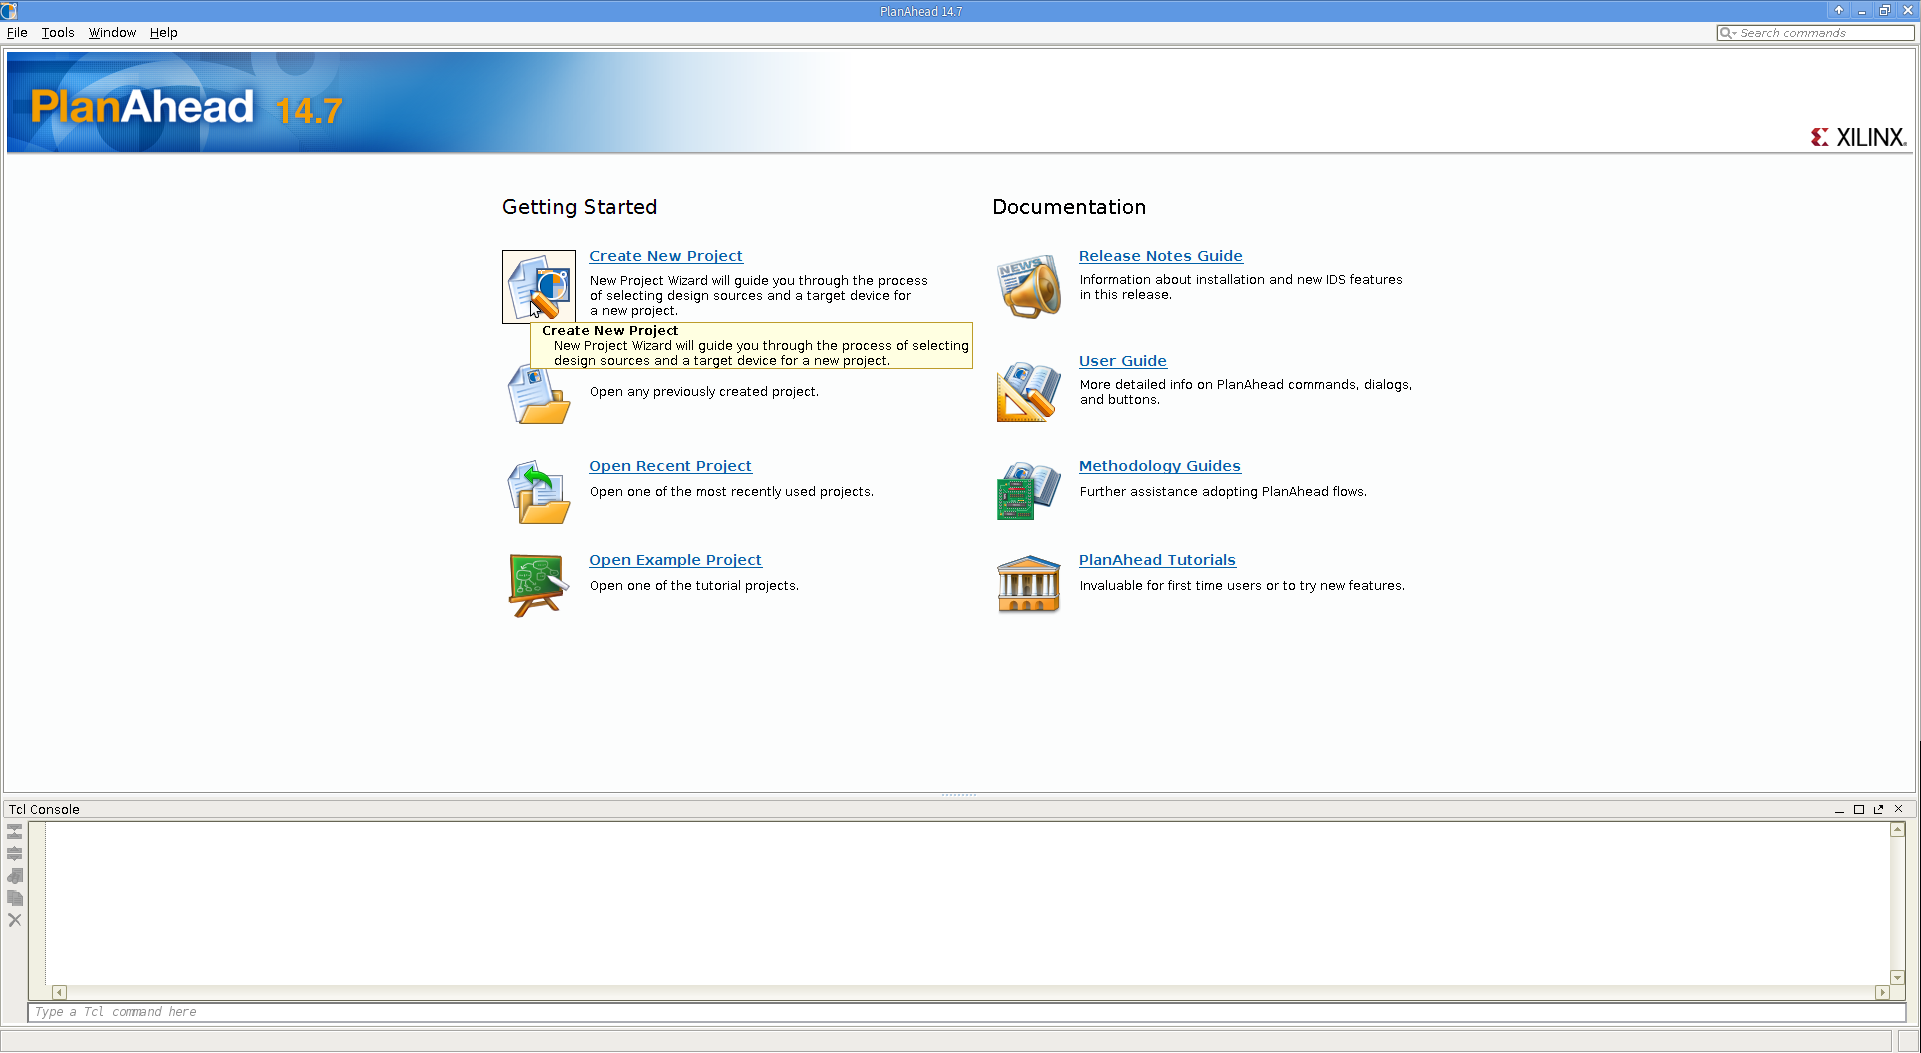
\includegraphics[scale=0.25]{pictures/PlanAheadOpenning.png}
	\caption{PlanAhead main window}
	\end{figure}
	\item In the first window, click next.
	\begin{figure}
	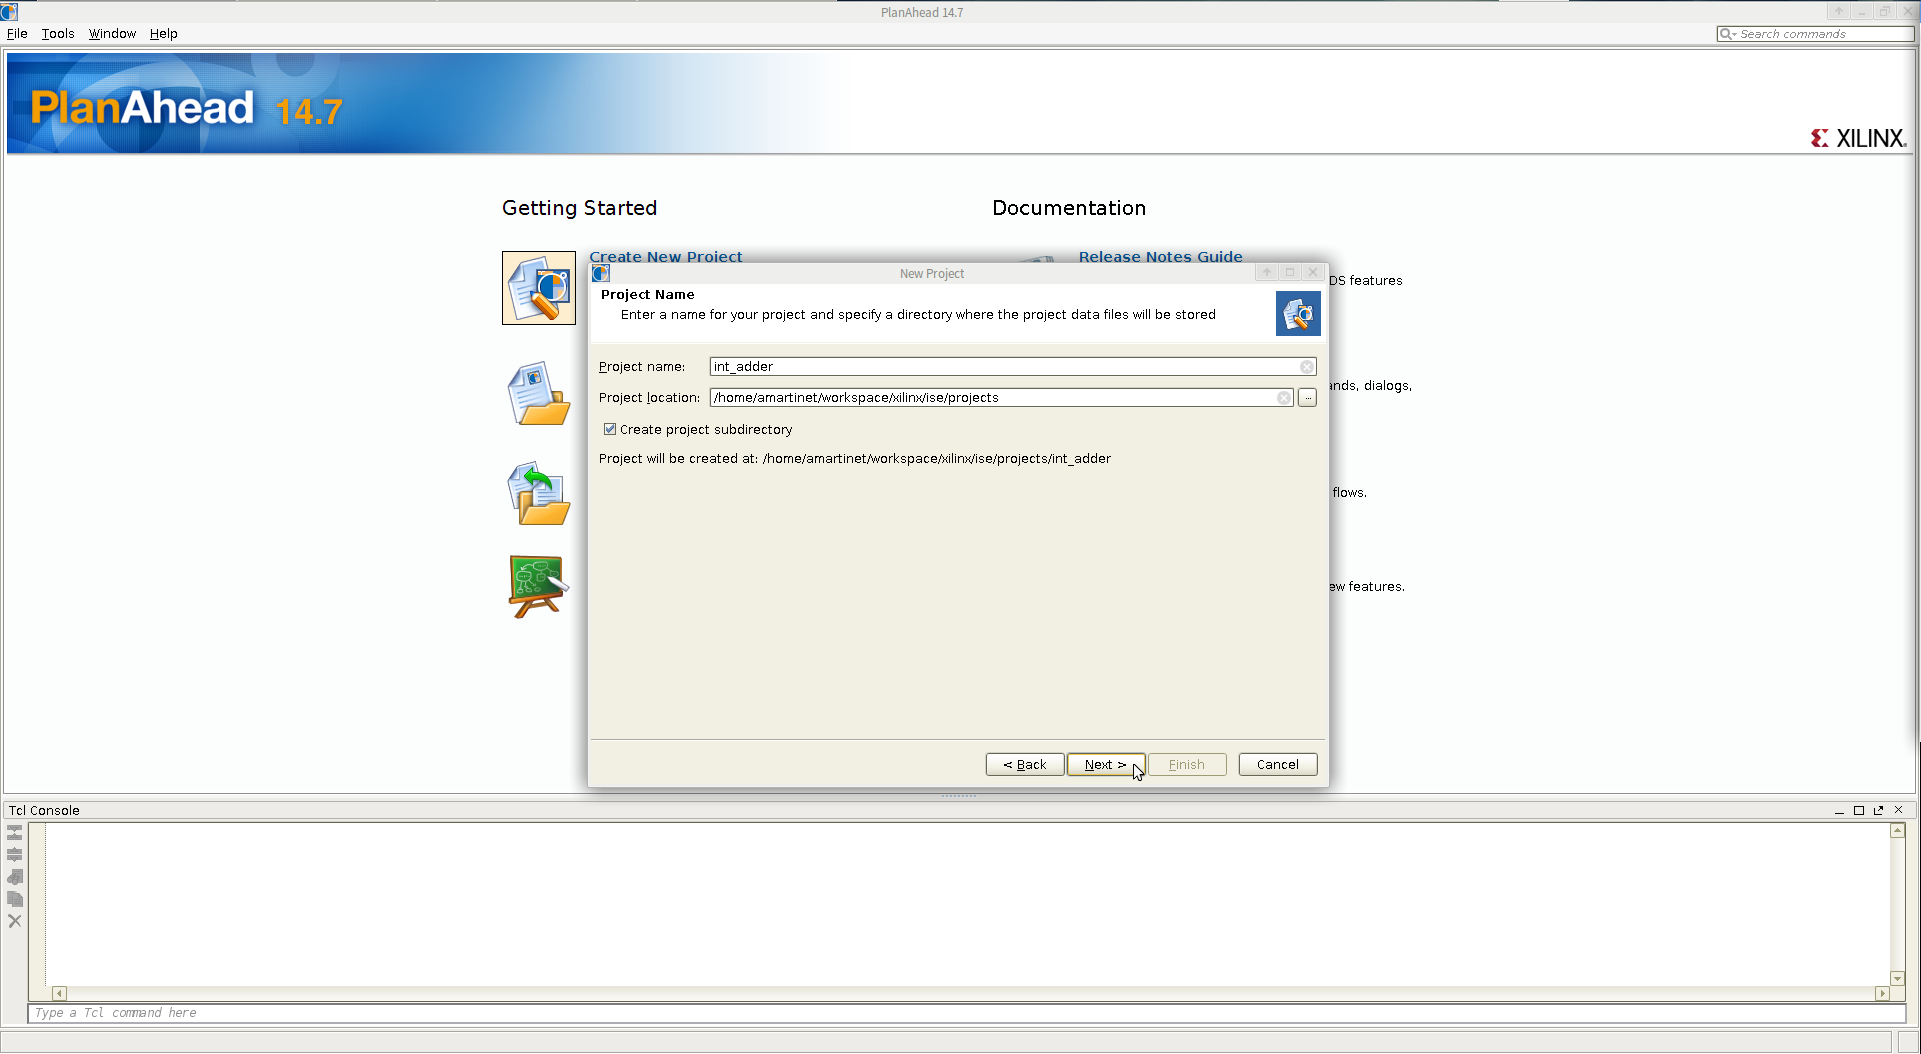
\includegraphics[scale=0.25]{pictures/CreateNewProject1.png}
	\caption{Create a new project}
	\end{figure}
	\item You're now asked to name and locate your new project. May I advise you to
	have a directory in which to put all your PlanAhead projects.
	Select your project location, and name your project, for example, I use
	"int\_adder". The box "Create project subdirectory" is checked. Leave it be.
	\begin{figure}
	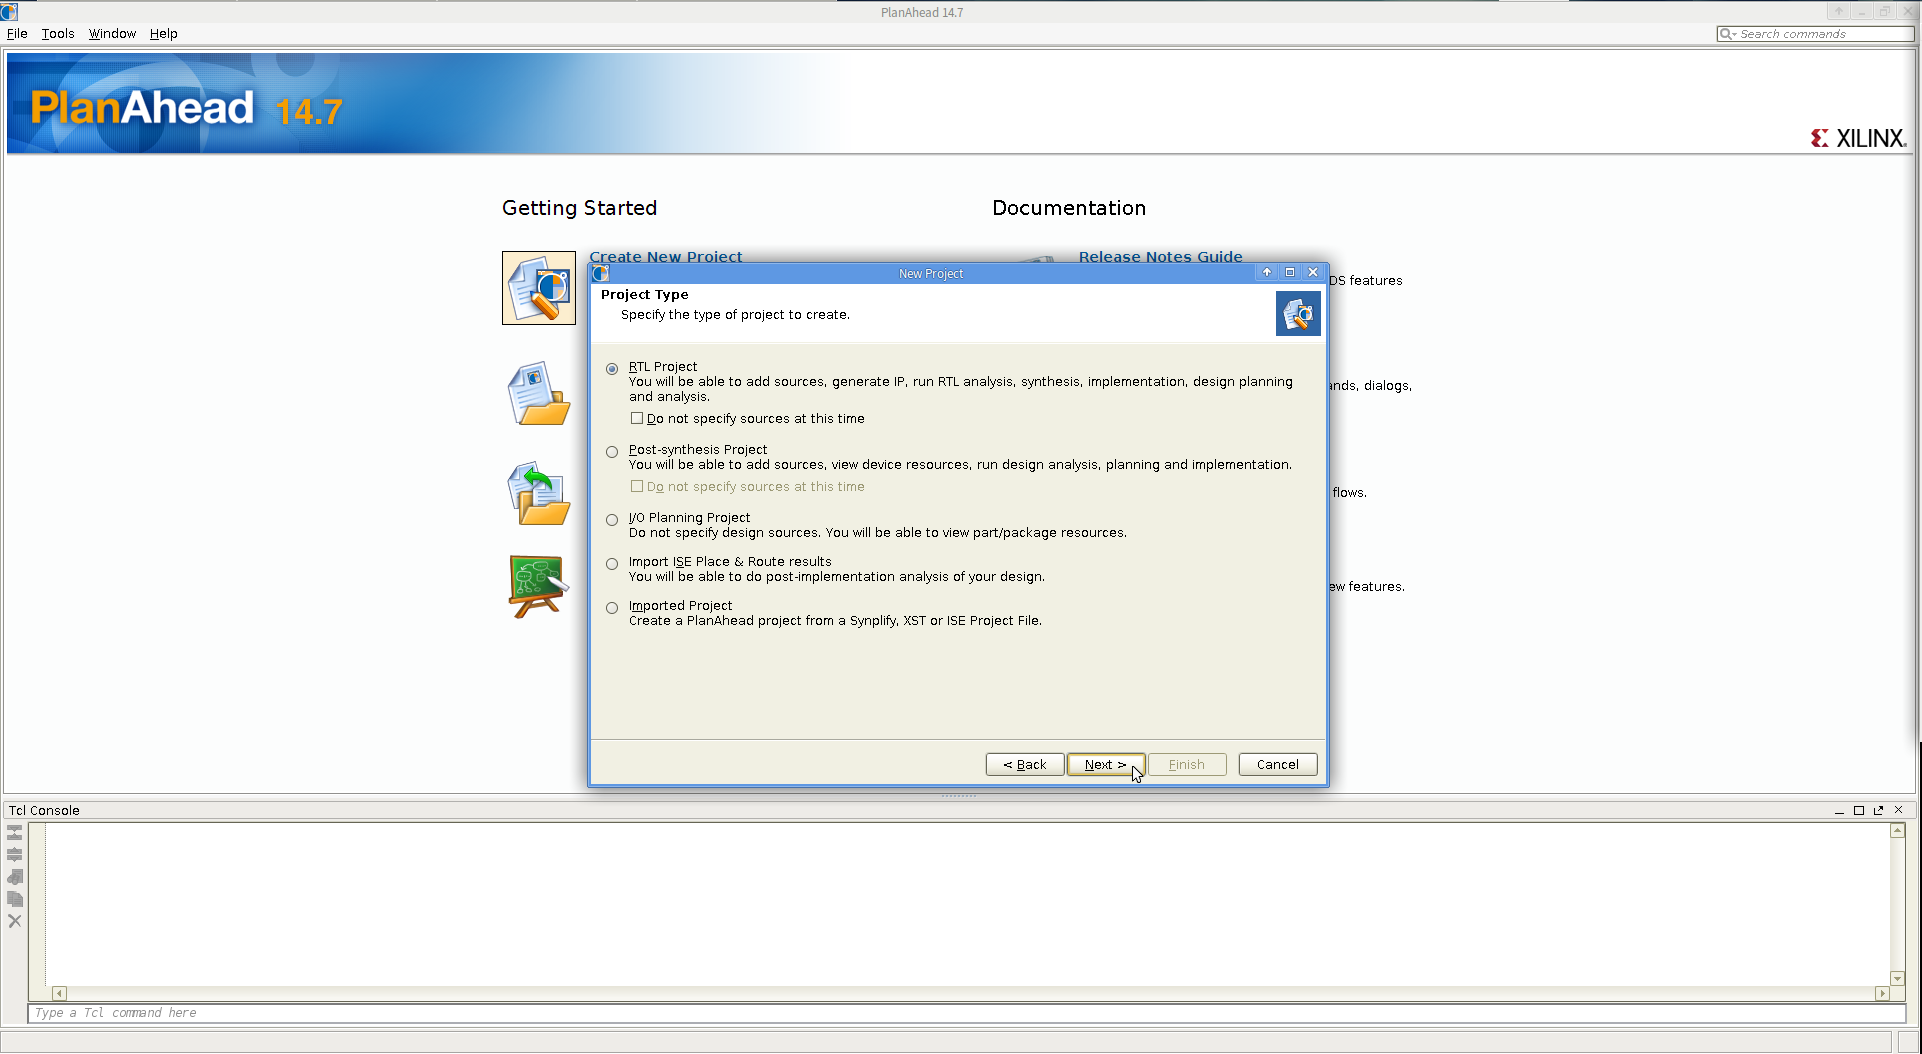
\includegraphics[scale=0.25]{pictures/CreateNewProject2.png}
	\caption{Create a new project}
	\end{figure}
	\item Click "Next".
	The button "RTL Project" is selectionned. Leave everything as it is. Click
	"Next".
	\begin{figure}
	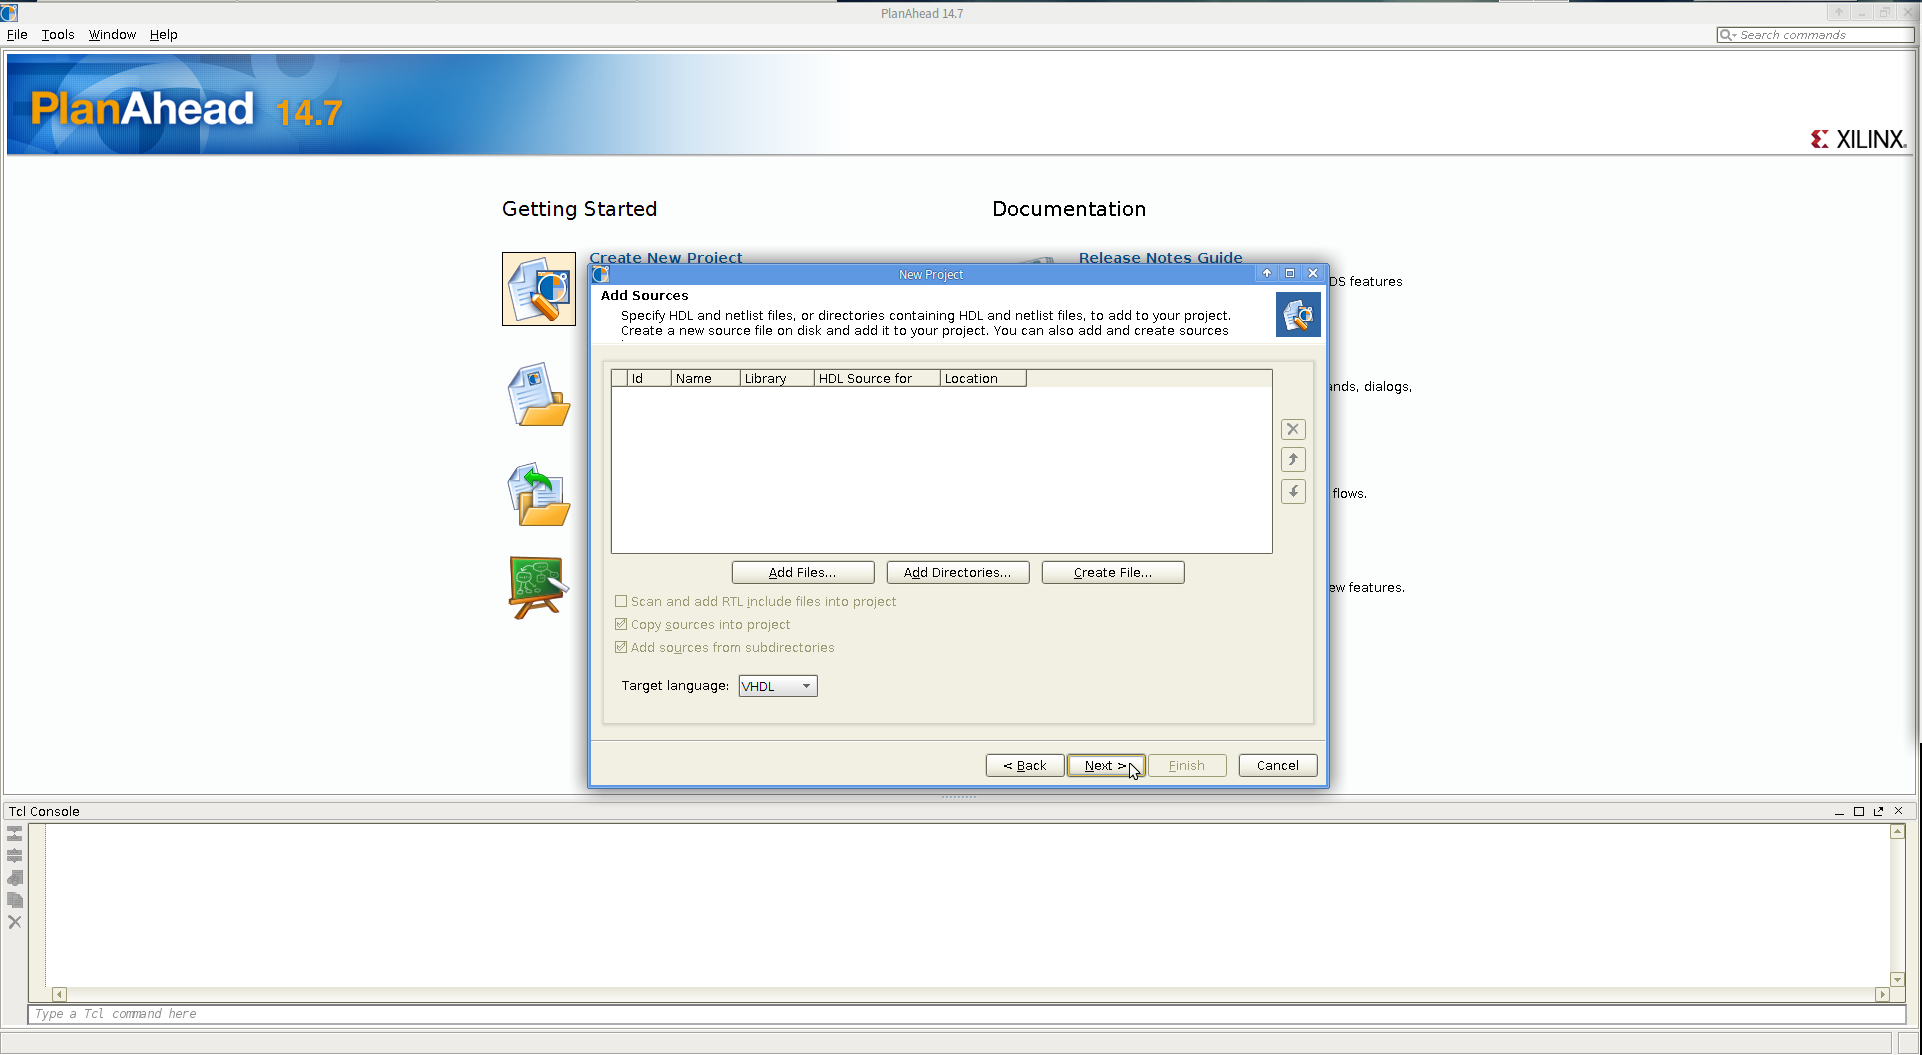
\includegraphics[scale=0.25]{pictures/CreateNewProject3.png}
	\caption{Create a new project}
	\end{figure}
	\item You get now to "Add Sources" screen. Set "Target language" to VHDL, as
	your entire design will be in VHDL, so it gives a better consistency.
	Actually, you could leave it to Verilog, as it will be recompiled and
	remixed by PlanAhead. As I don't know verilog very well, I prefer VHDL in
	case of improbable bug issues to fix.
	\begin{figure}
	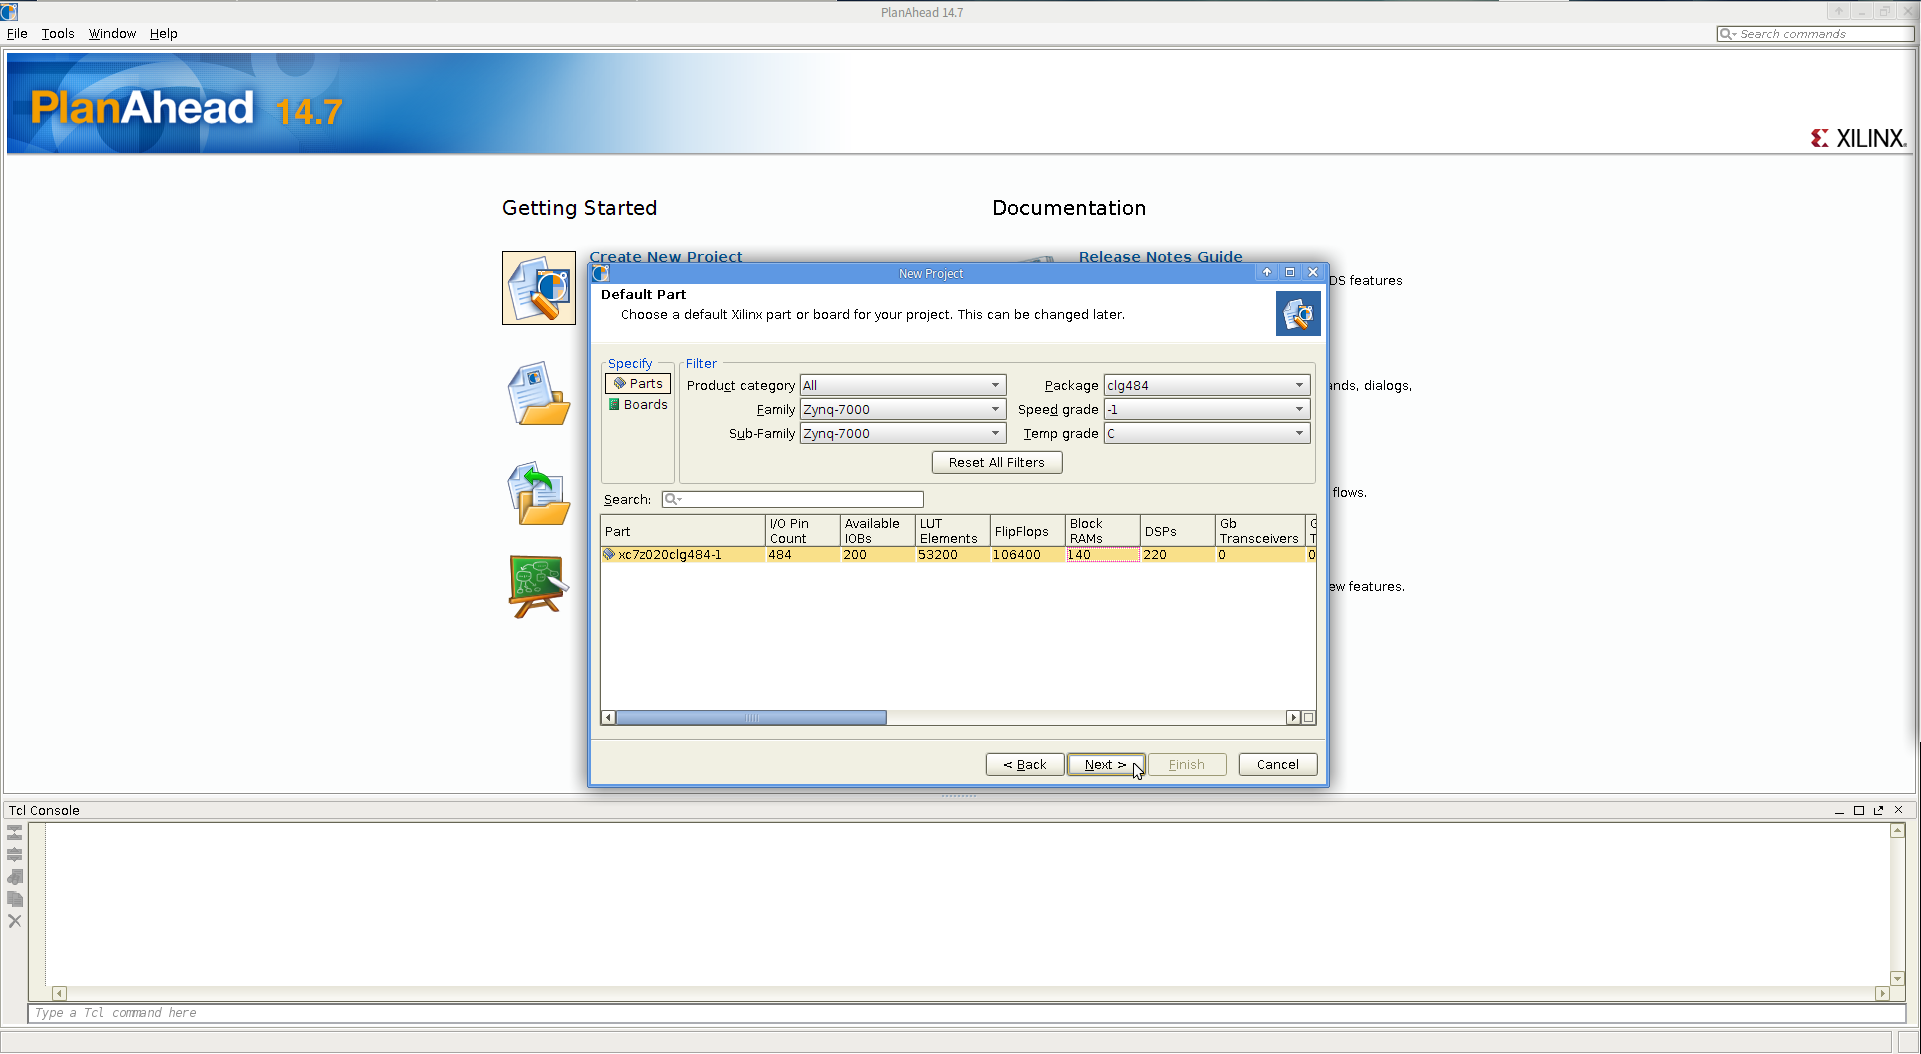
\includegraphics[scale=0.25]{pictures/CreateNewProject4.png}
	\caption{Create a new project}
	\end{figure}
	\item Click "Next".
	\item You get to "Add Existing IP" screen. Nothing to do. Click "Next".
	\item You can here add constraints. But we do not have any constraint file	to add for the moment. Click "Next".
	\item Then you get to "Default Part" screen. Here you will choose the
	hardware specifications. To choose your part, you may need some filters as
	the names are not user-readable.
	\begin{itemize}
		\item In "Family" field, select "Zynq-7000"
		\item In "Sub-Family" field, select "Zynq-7000"
		\item In "Package" field, select "clg484" as it is the package type of
		your chip (see zedboard documentation).
		\item In "Speed grade" field, select "-1" as you don't need to get in speed details for the moment.
		\item Leave the "Temp grade" field for the moment.
	\end{itemize}
	\begin{figure}
	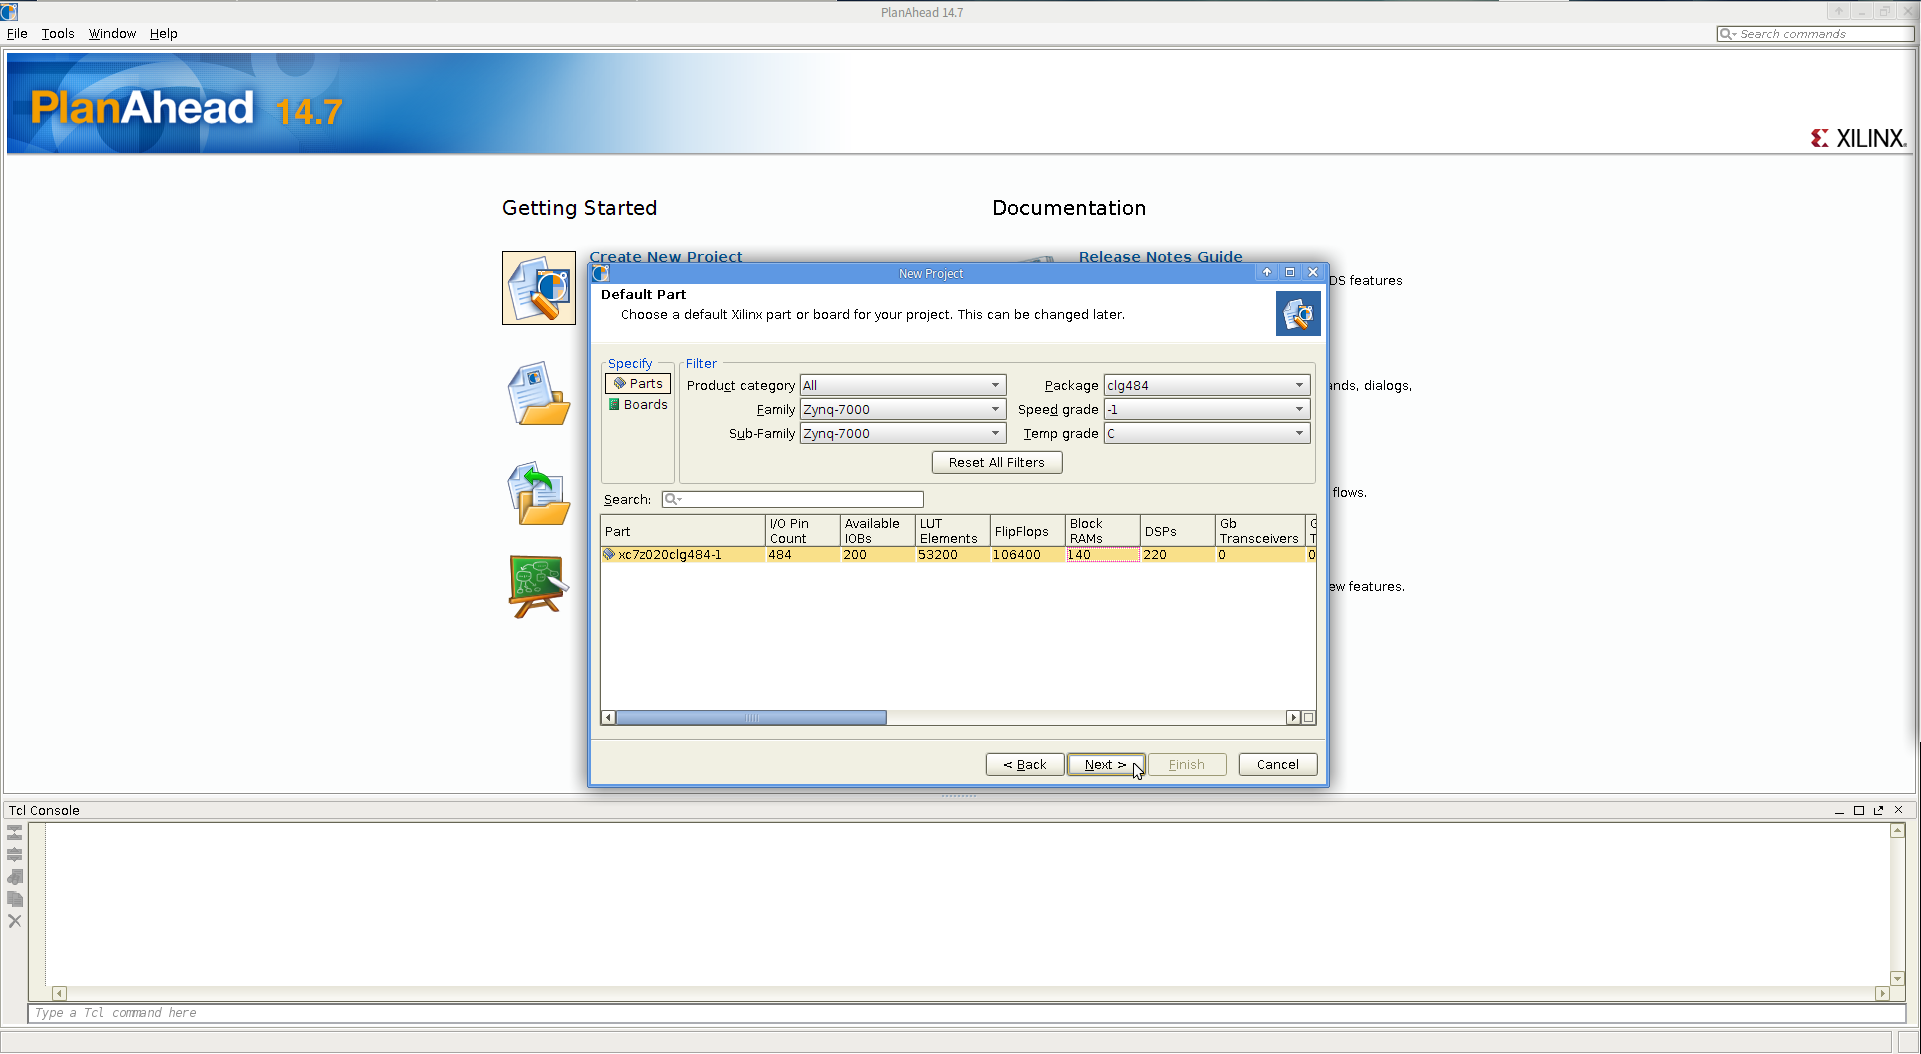
\includegraphics[scale=0.25]{pictures/CreateNewProject4.png}
	\caption{Create a new project}
	\end{figure}
	Then only one part should remain, xc7z020clg484-1. You will see on ZedBoard
	documentation that this is actually the name of the chip. Double-click on it
	or click "Next".
	\item You get now to the project summary. Click "Finish" to create the new
	project. The project creation process may take a short time to complete.
	\begin{figure}
	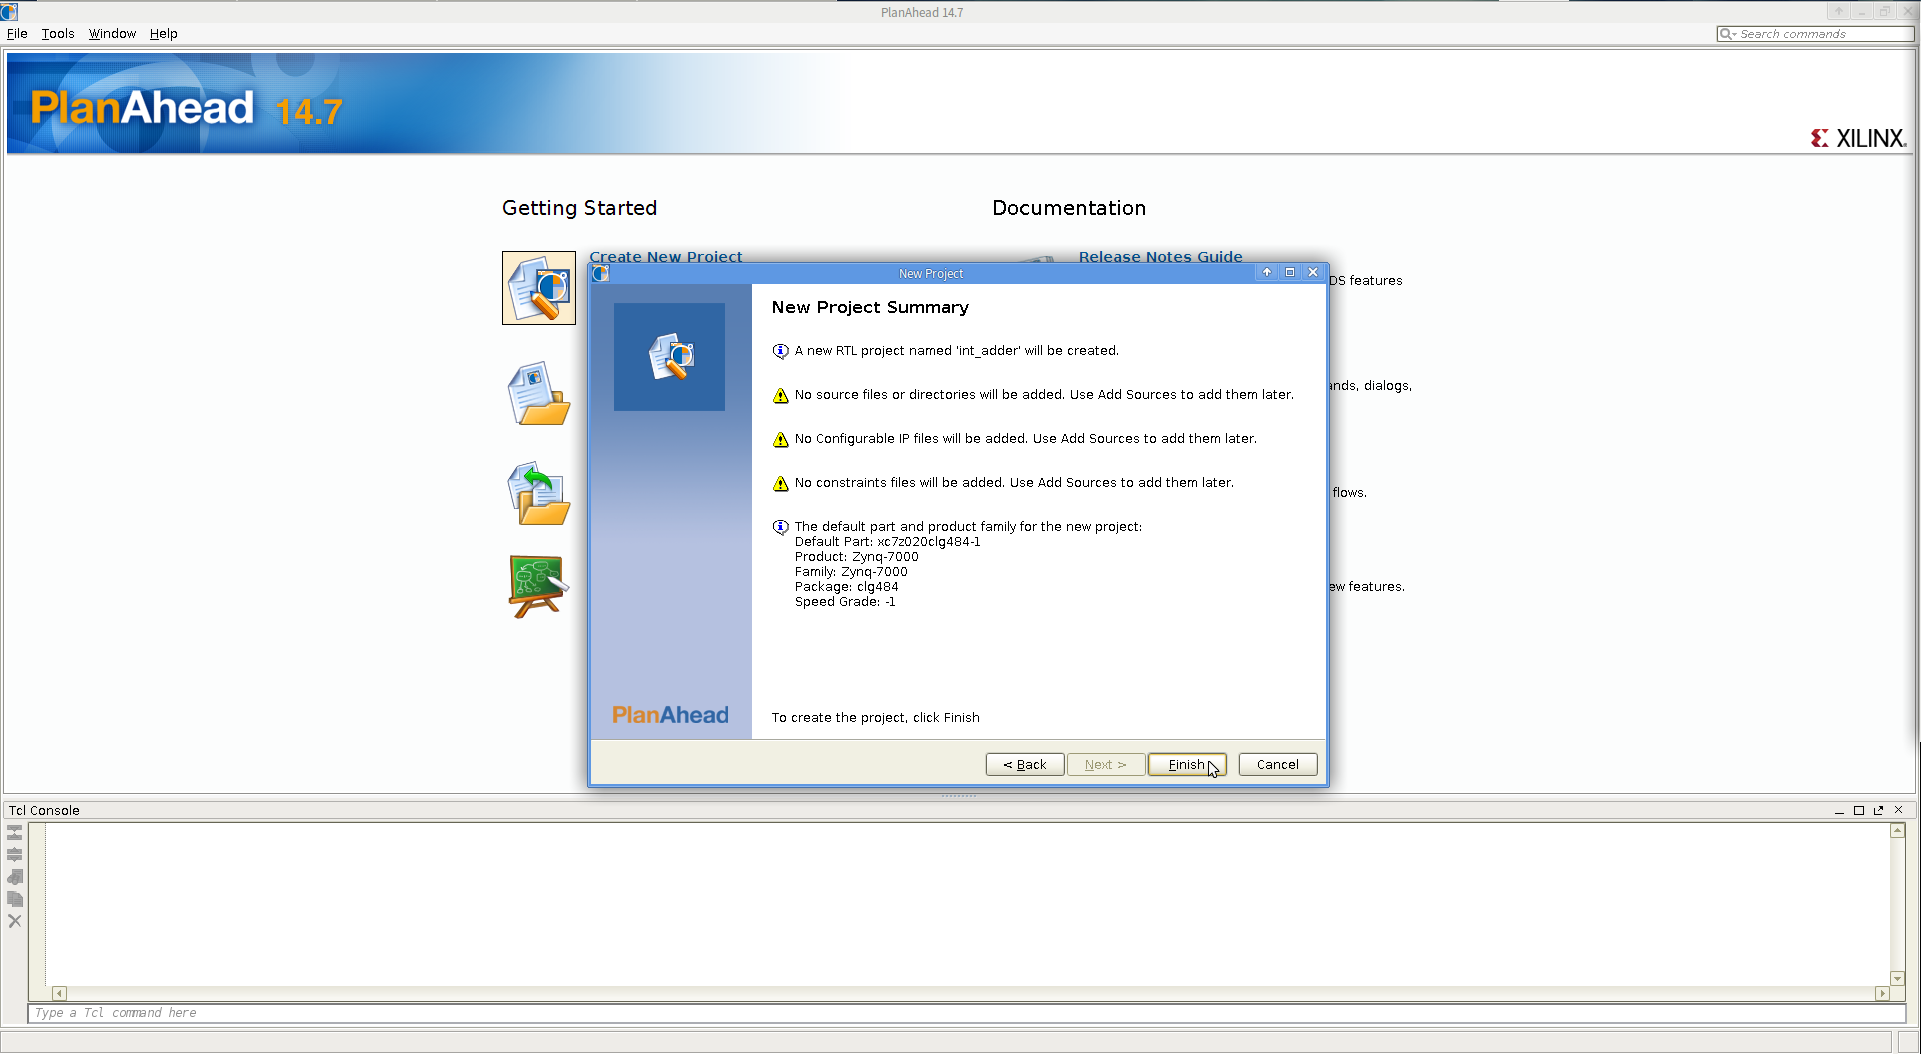
\includegraphics[scale=0.25]{pictures/CreateNewProject5.png}
	\caption{Create a new project}
	\end{figure}
	\end{enumerate}

	Then we will get to the hardware design on XPS.

	\subsection{Hardware design on XPS}
	Now you have to create an embedded source to design the hardware.
	\begin{enumerate}
	\item In the flow navigator (by default on the left panel), click "Add
	\begin{figure}
	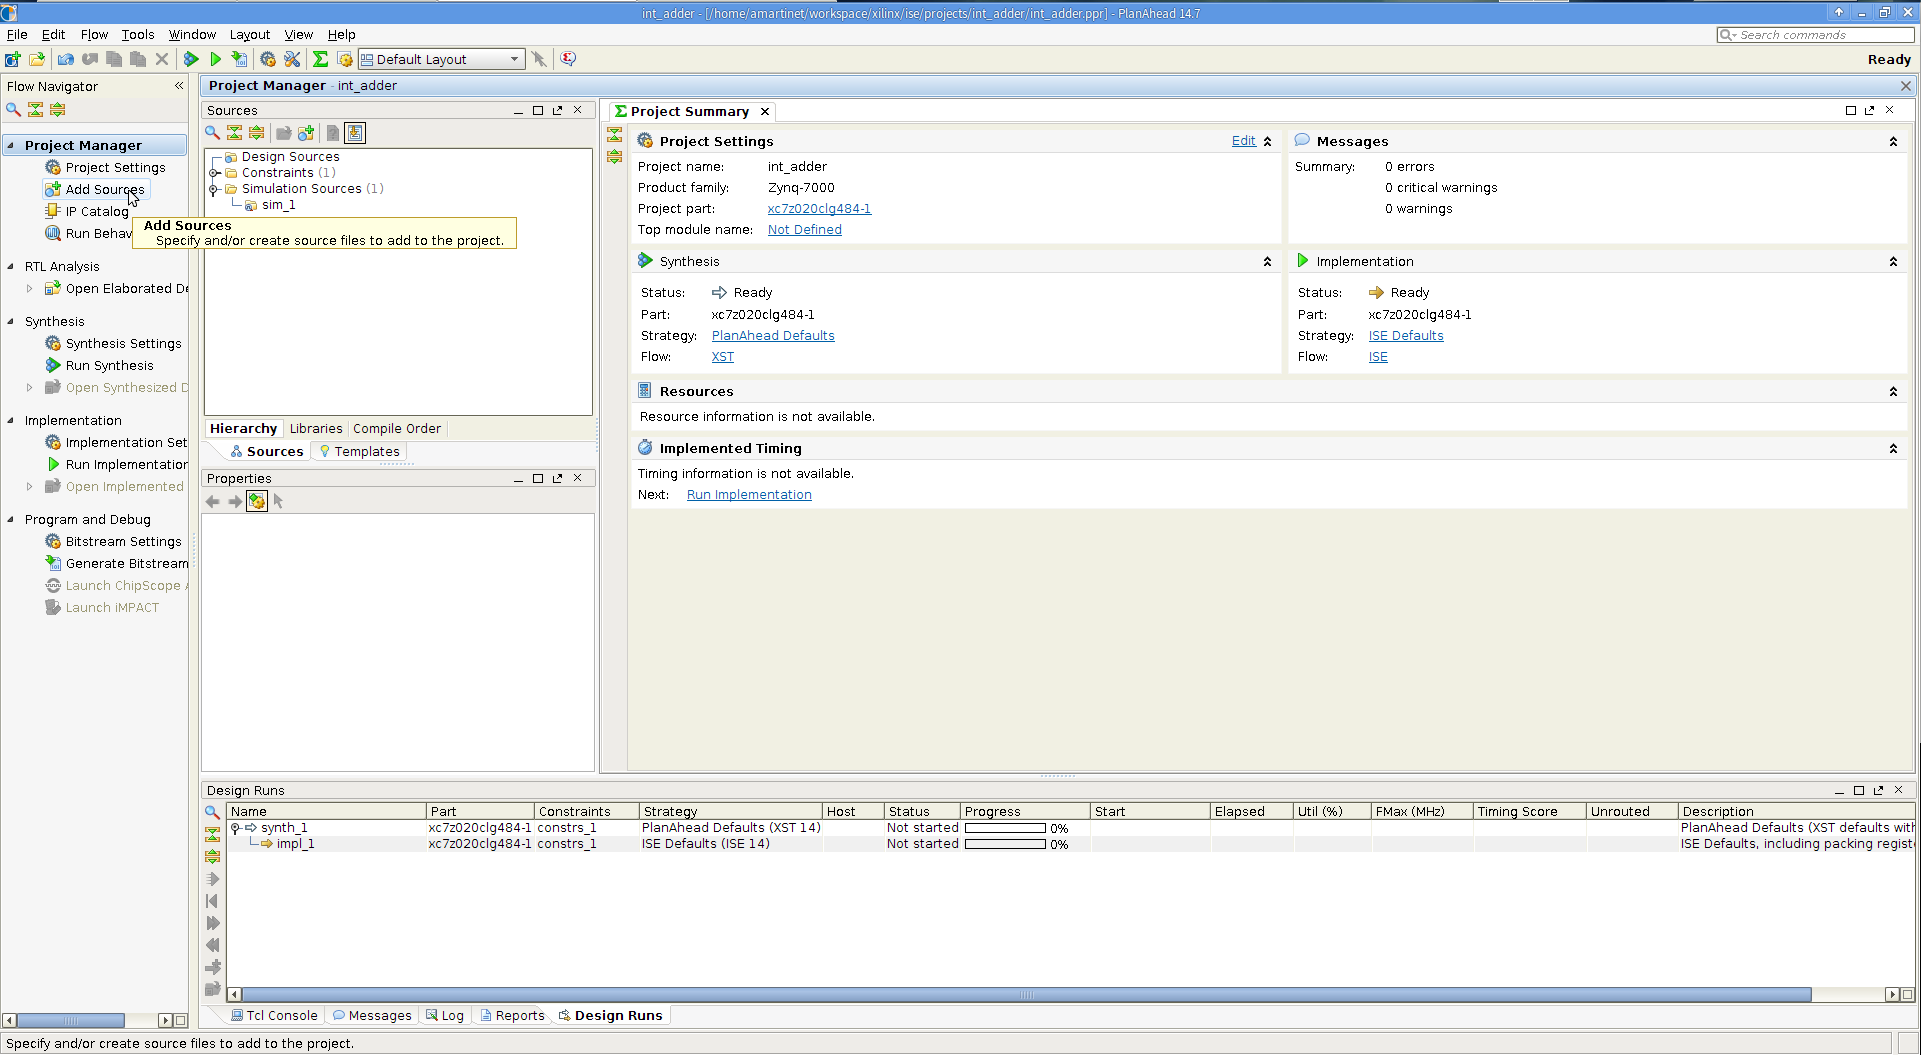
\includegraphics[scale=0.25]{pictures/AddSources1.png}
	\caption{Add sources: create sub-design}
	\end{figure}
	Sources" in the "Project Manager" menu.
	\item In the "Add Sources" window that popped up, select "Add or Create
	Embedded Sources" and click "Next".
	\begin{figure}
	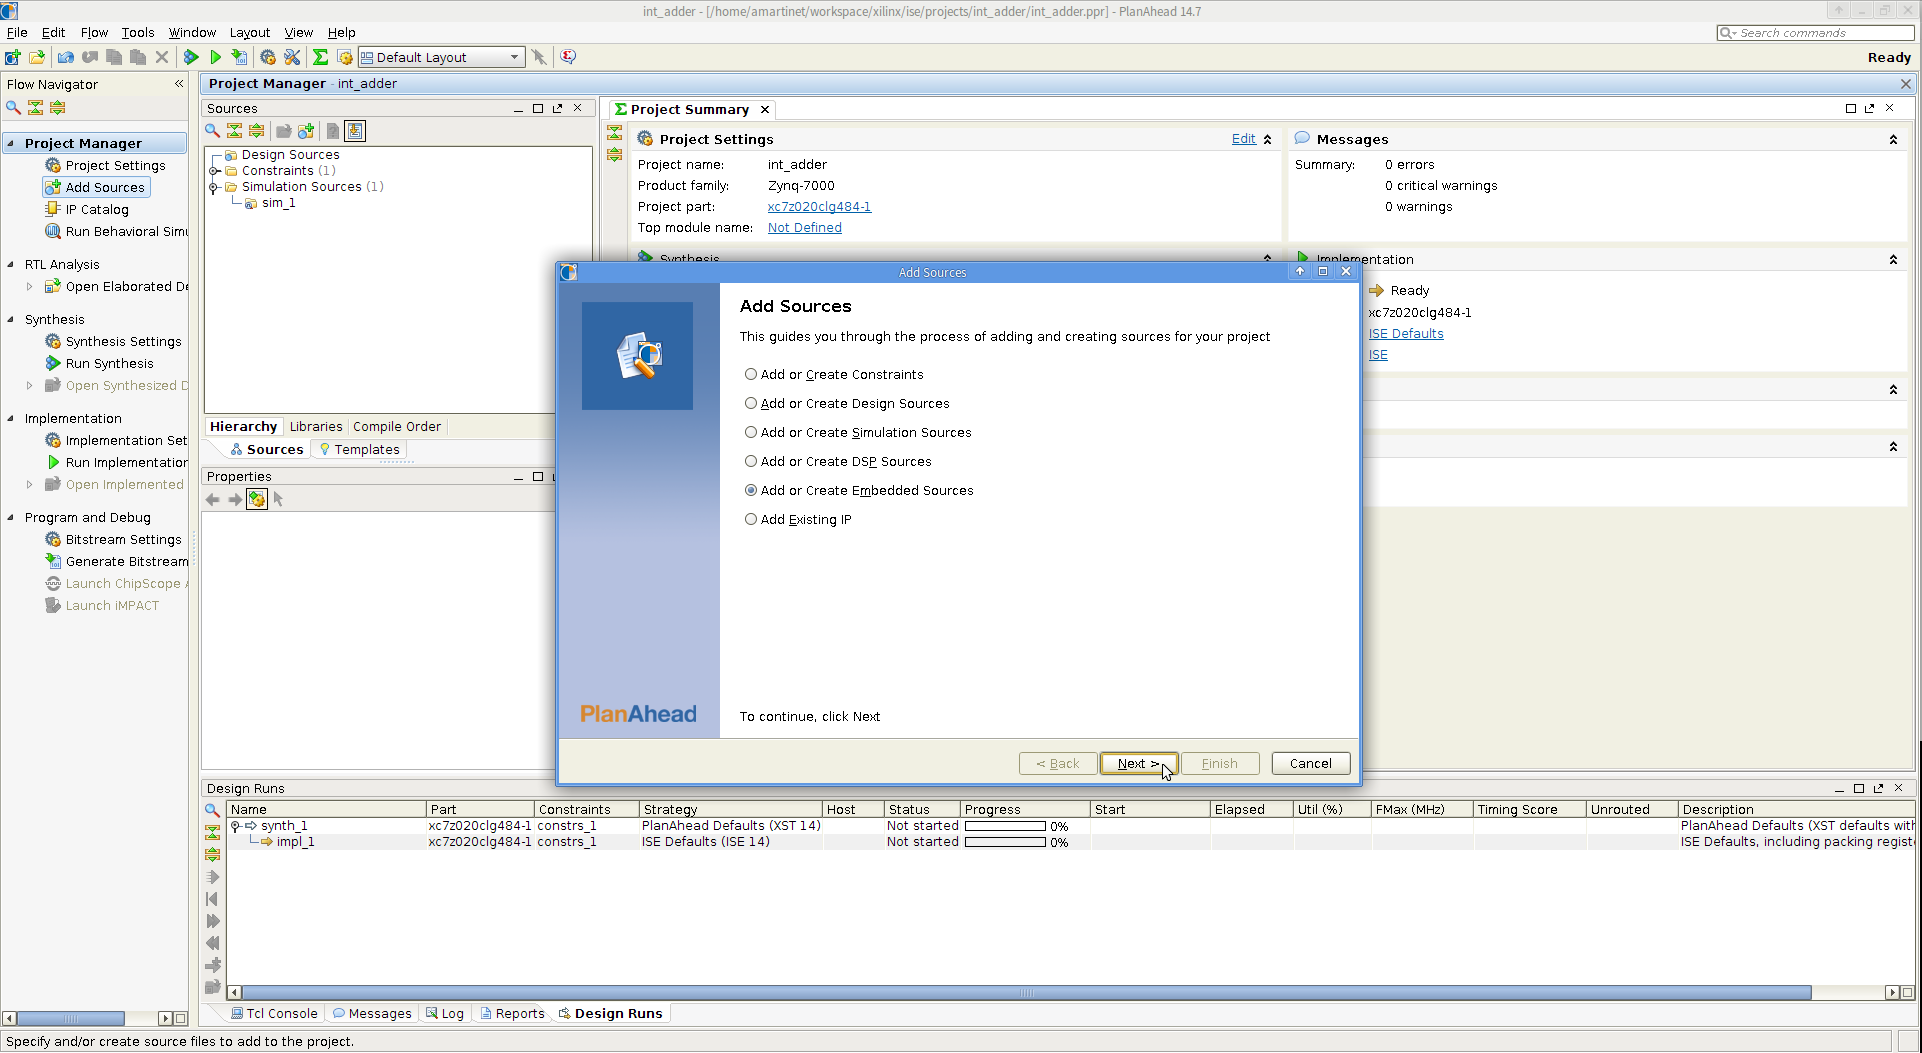
\includegraphics[scale=0.25]{pictures/AddSources2.png}
	\caption{Add sources: create sub-design}
	\end{figure}
	\item Then click "Create Sub-Design". Name your embedded source, for
	example, I used "system". Click "OK".
	\begin{figure}
	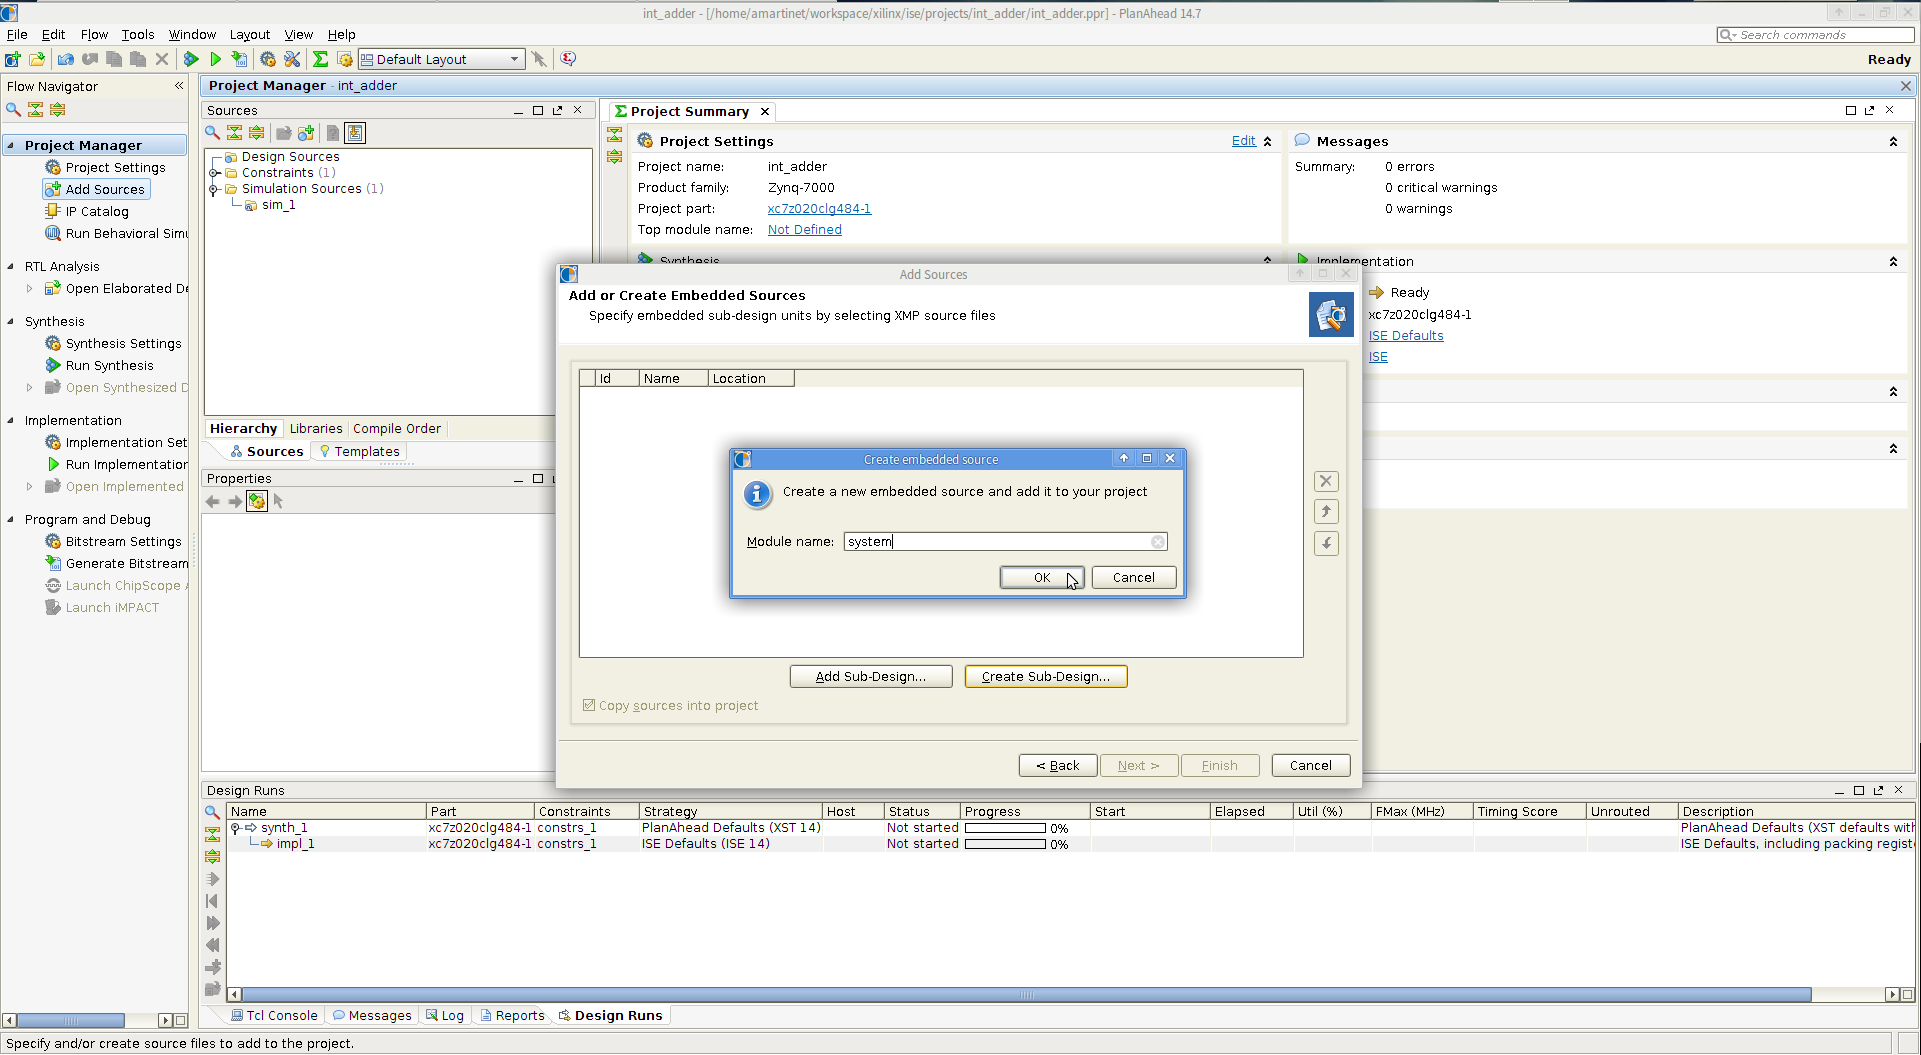
\includegraphics[scale=0.25]{pictures/AddSources3.png}
	\caption{Add sources: create sub-design}
	\end{figure}
	\item You will see the new file system.xmp pop as first line of the embedded
	\begin{figure}
	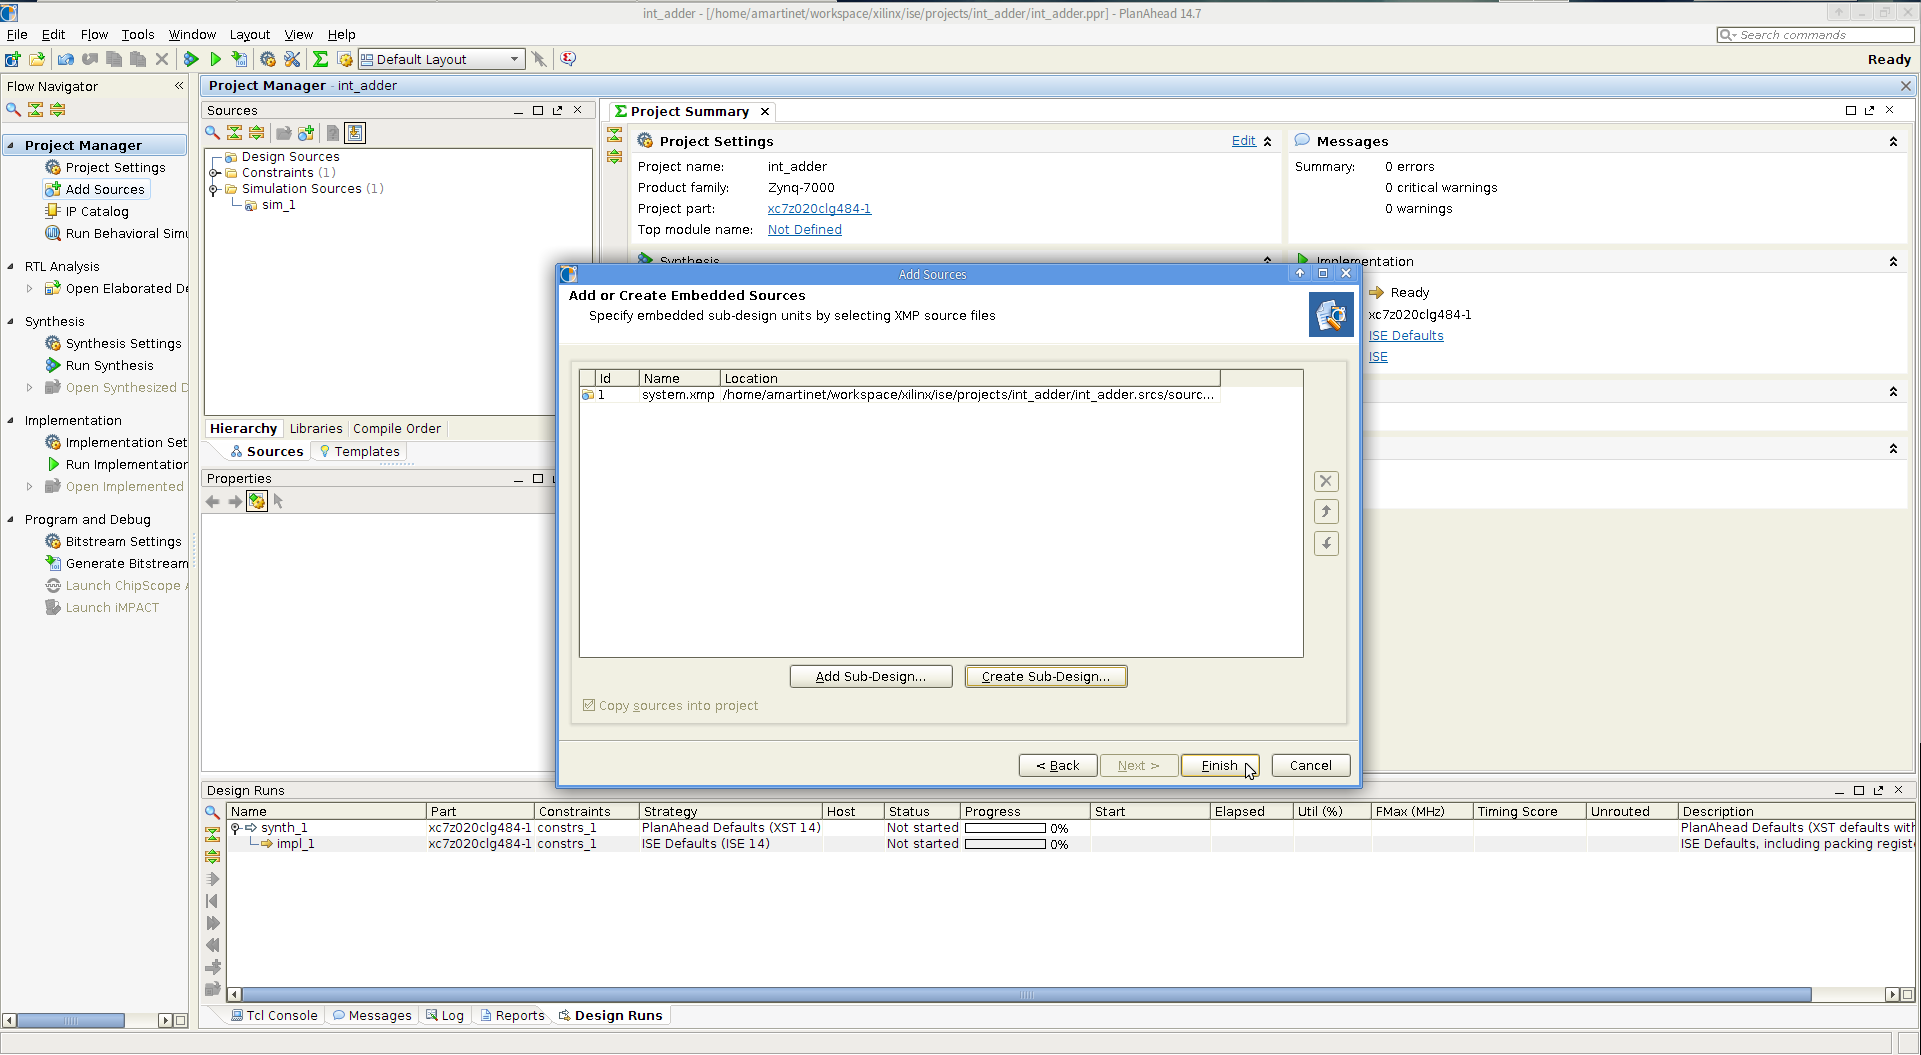
\includegraphics[scale=0.25]{pictures/AddSources4.png}
	\caption{Add sources: create sub-design}
	\end{figure}
	sources table. Click "Finish". XPS Launches after a while.
	\item XPS will ask you if you want to add a Processing System 7 instance to
	the system. Click "Yes". Wait for a while.
	\begin{figure}
	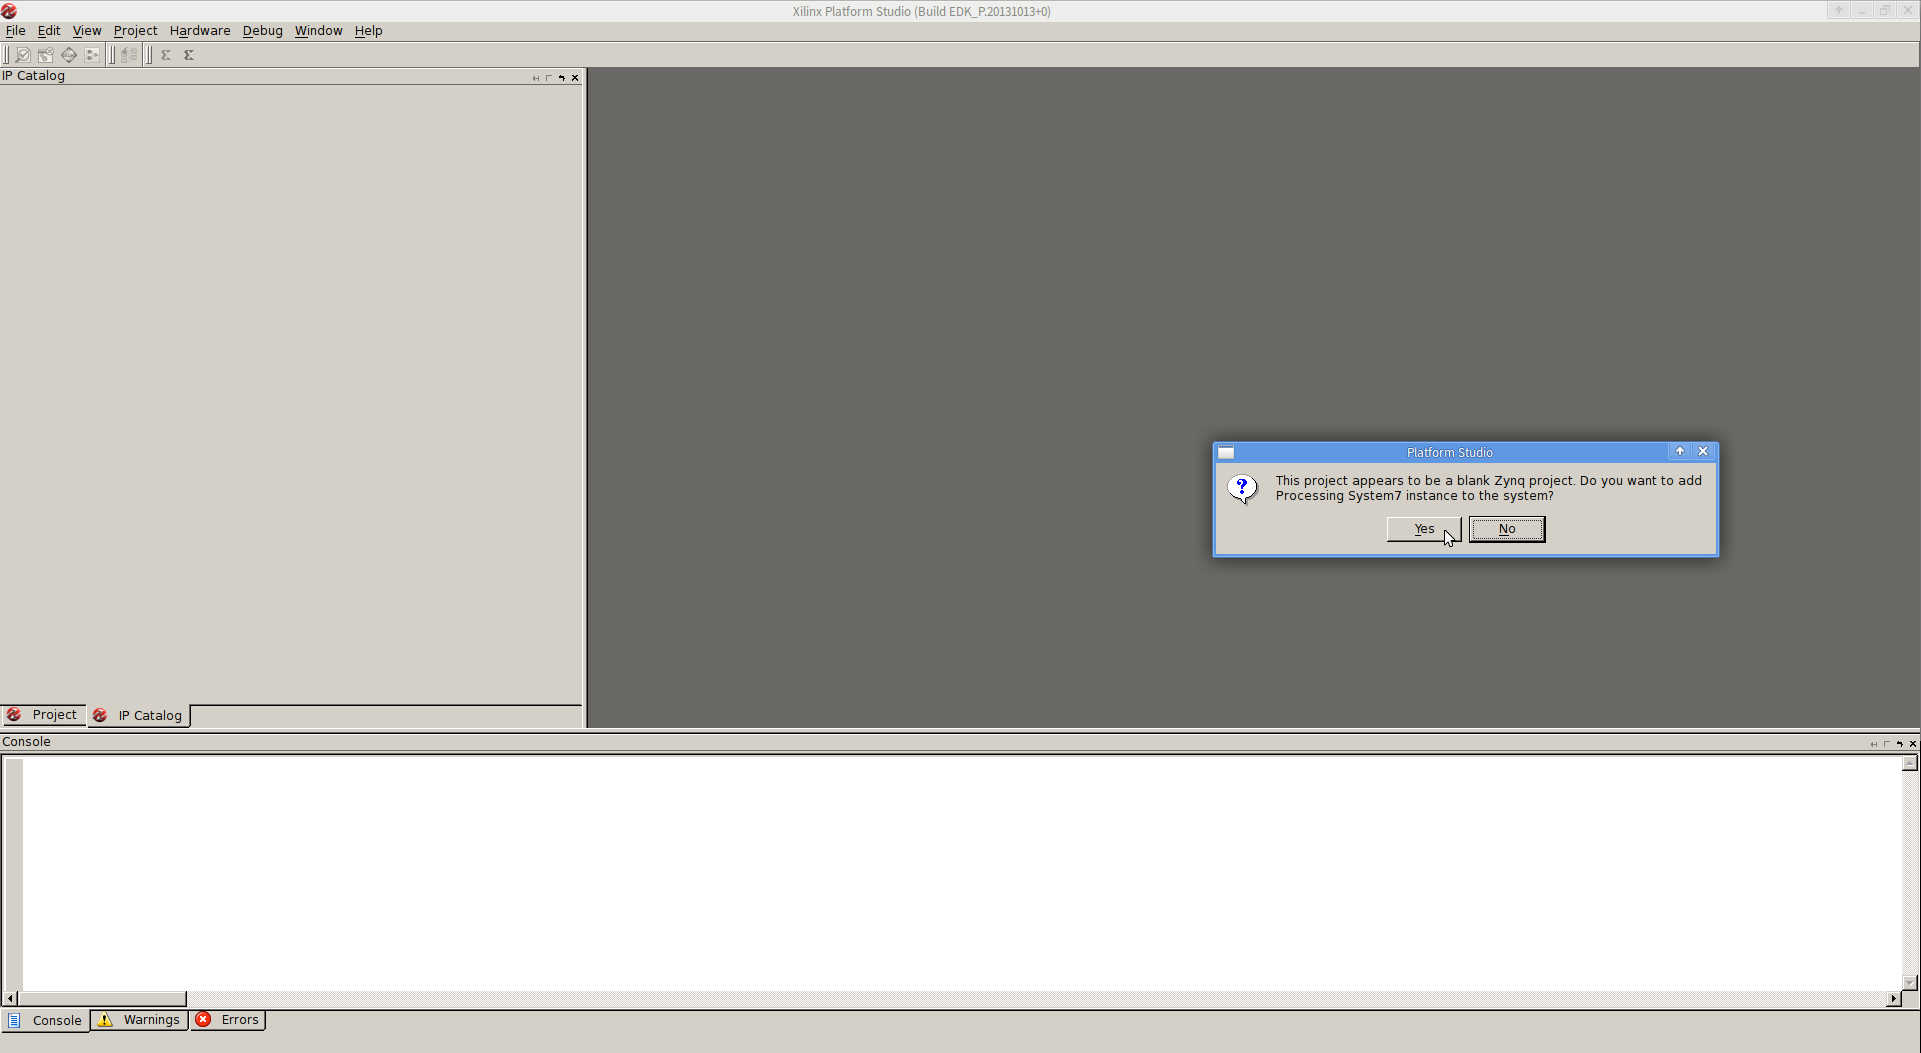
\includegraphics[scale=0.25]{pictures/XPSlaunch.png}
	\caption{XPS launch}
	\end{figure}
	\item Then you have to load the basic configuration of the PS. Note that
	every settings are note important for the job we are performing, but some
	configuration features, as UART and USB, are useful to see the displayed
	results of preograms on a tty for example.
	In the zynq tab, click "Import".
	\begin{figure}
	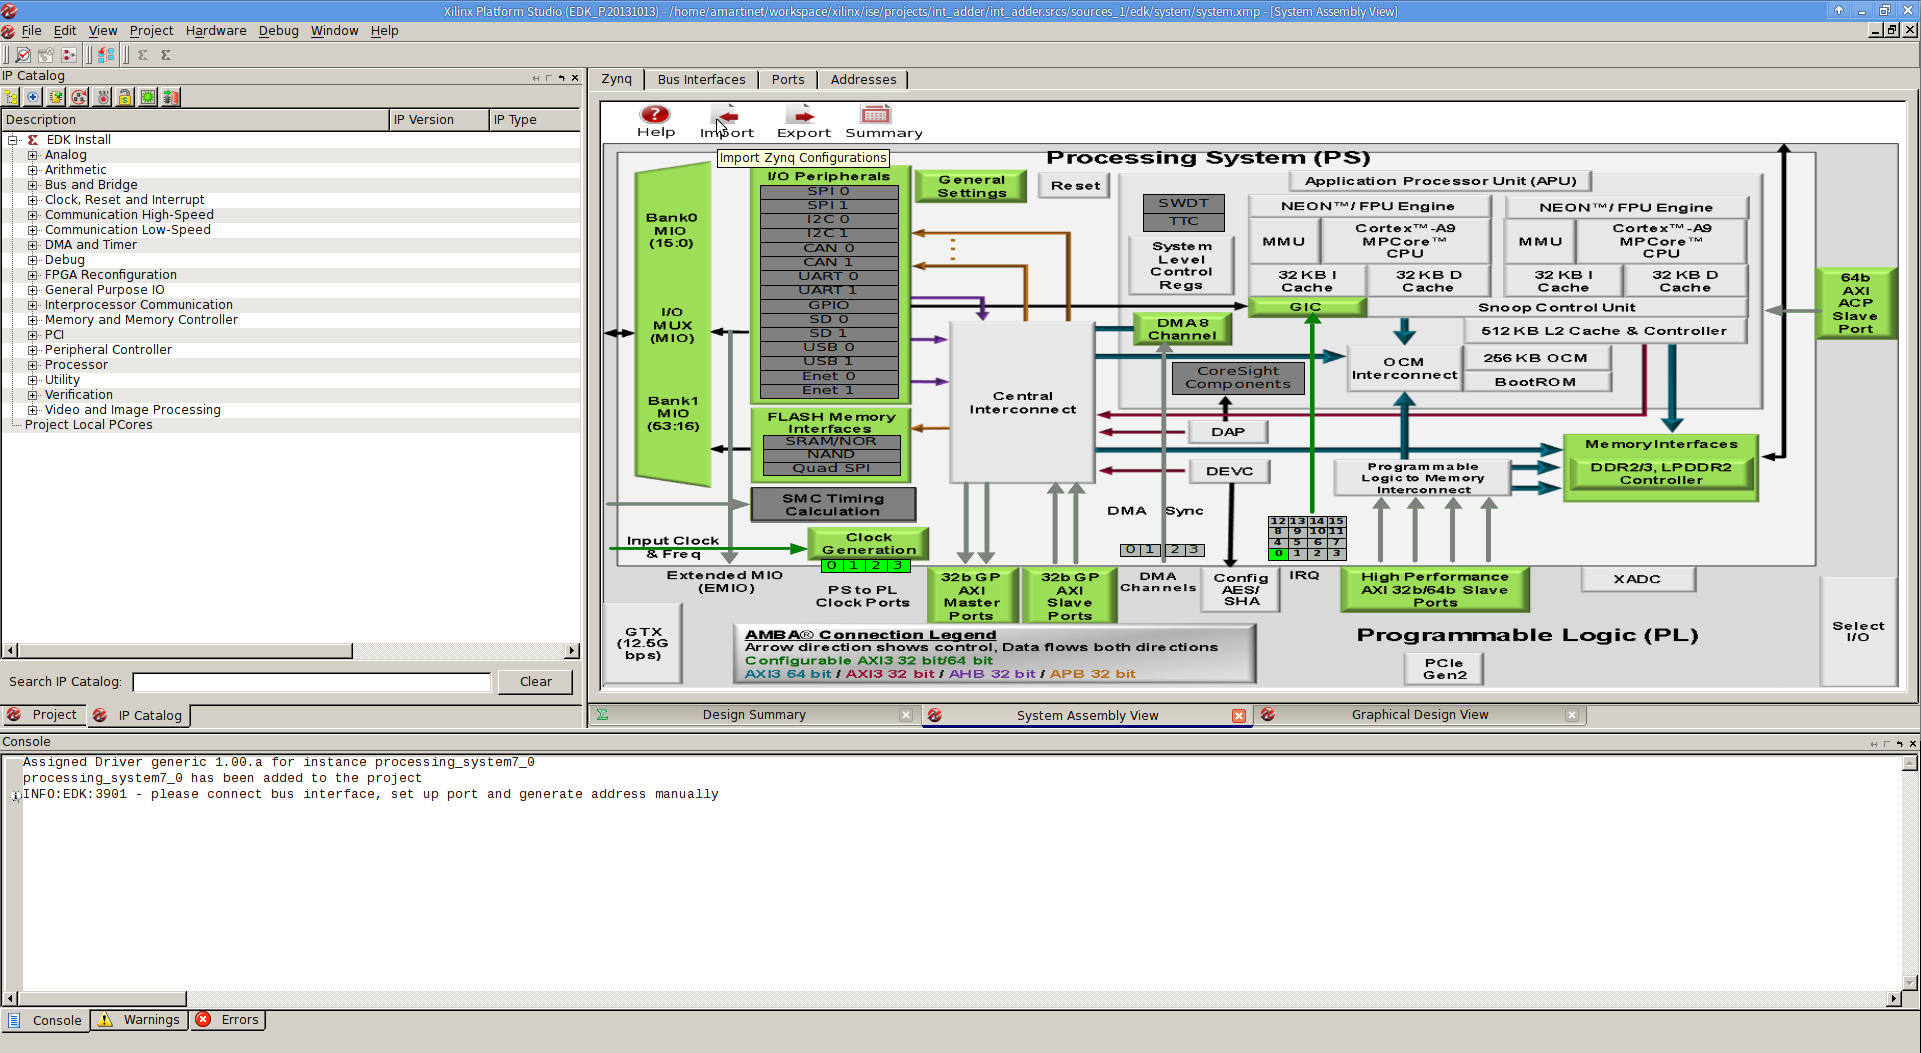
\includegraphics[scale=0.25]{pictures/XPSImport1.png}
	\caption{Import Configuration}
	\end{figure}
	\item In the User Template list, click on the "+" button, browse the file
	zedboard\_RevC\_v2.xml.
	You can download it here:\\
		\url{http://zedboard.org/sites/default/files/documentations/zedboard_RevC_v2_XML.zip}
	\begin{figure}
	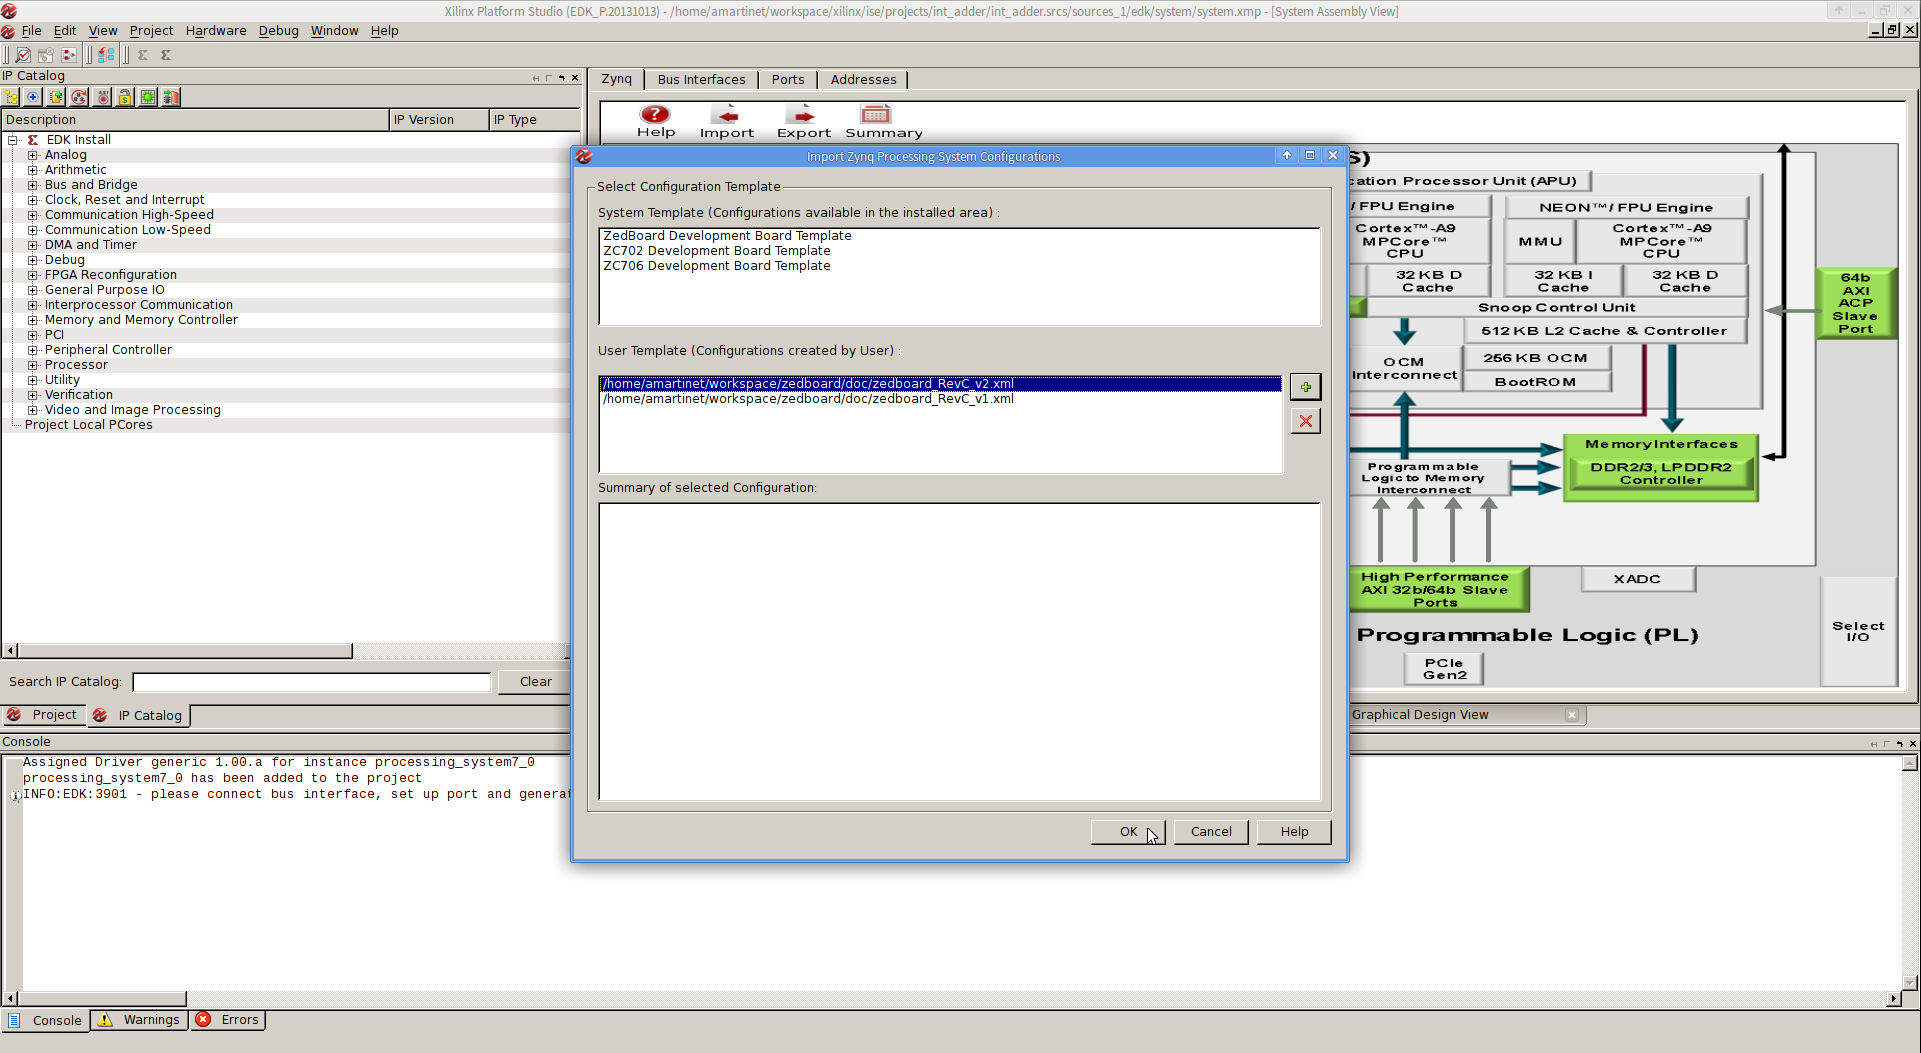
\includegraphics[scale=0.25]{pictures/XPSImport2.png}
	\caption{Import Configuration}
	\end{figure}
	\item click "OK"
	\item XPS may ask you if you want to continue importing and updating MIO
	configuration. Click "Yes".
	\begin{figure}
	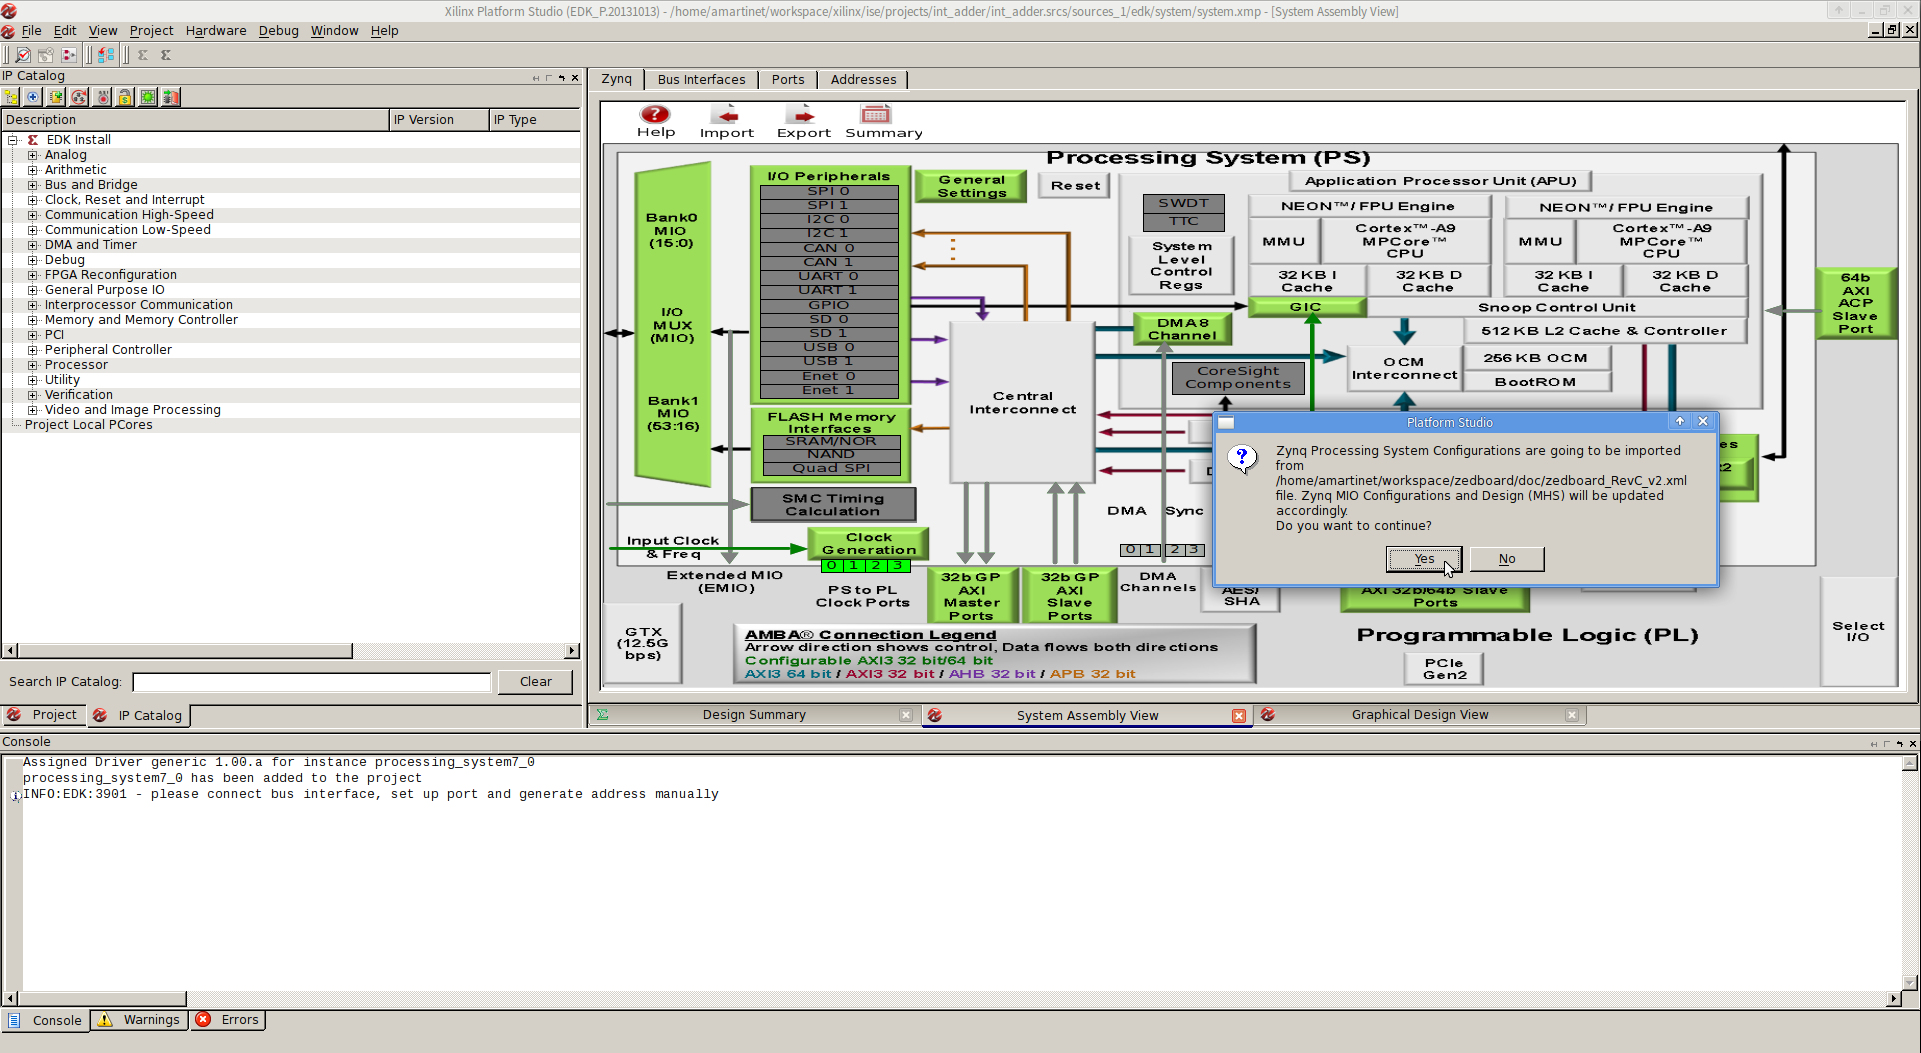
\includegraphics[scale=0.25]{pictures/XPSImport3.png}
	\caption{Import Configuration}
	\end{figure}
	\item Now, we are going to set the width of GPIO we are using. As we can
	read in the ZedBoard documentation, Custom PL peripherals have to be mapped
	through EMIO on the GPIO banks 2 and 3. For more info about GPIOs, you can
	go to \hyperref[sec:GPIOSG]{ appendix \ref{sec:GPIOSG}: \nameref{sec:GPIOSG} }.
	\begin{itemize}
		\item So, in the Zynq tab, click on "I/O Peripherals" green box.
	\begin{figure}
	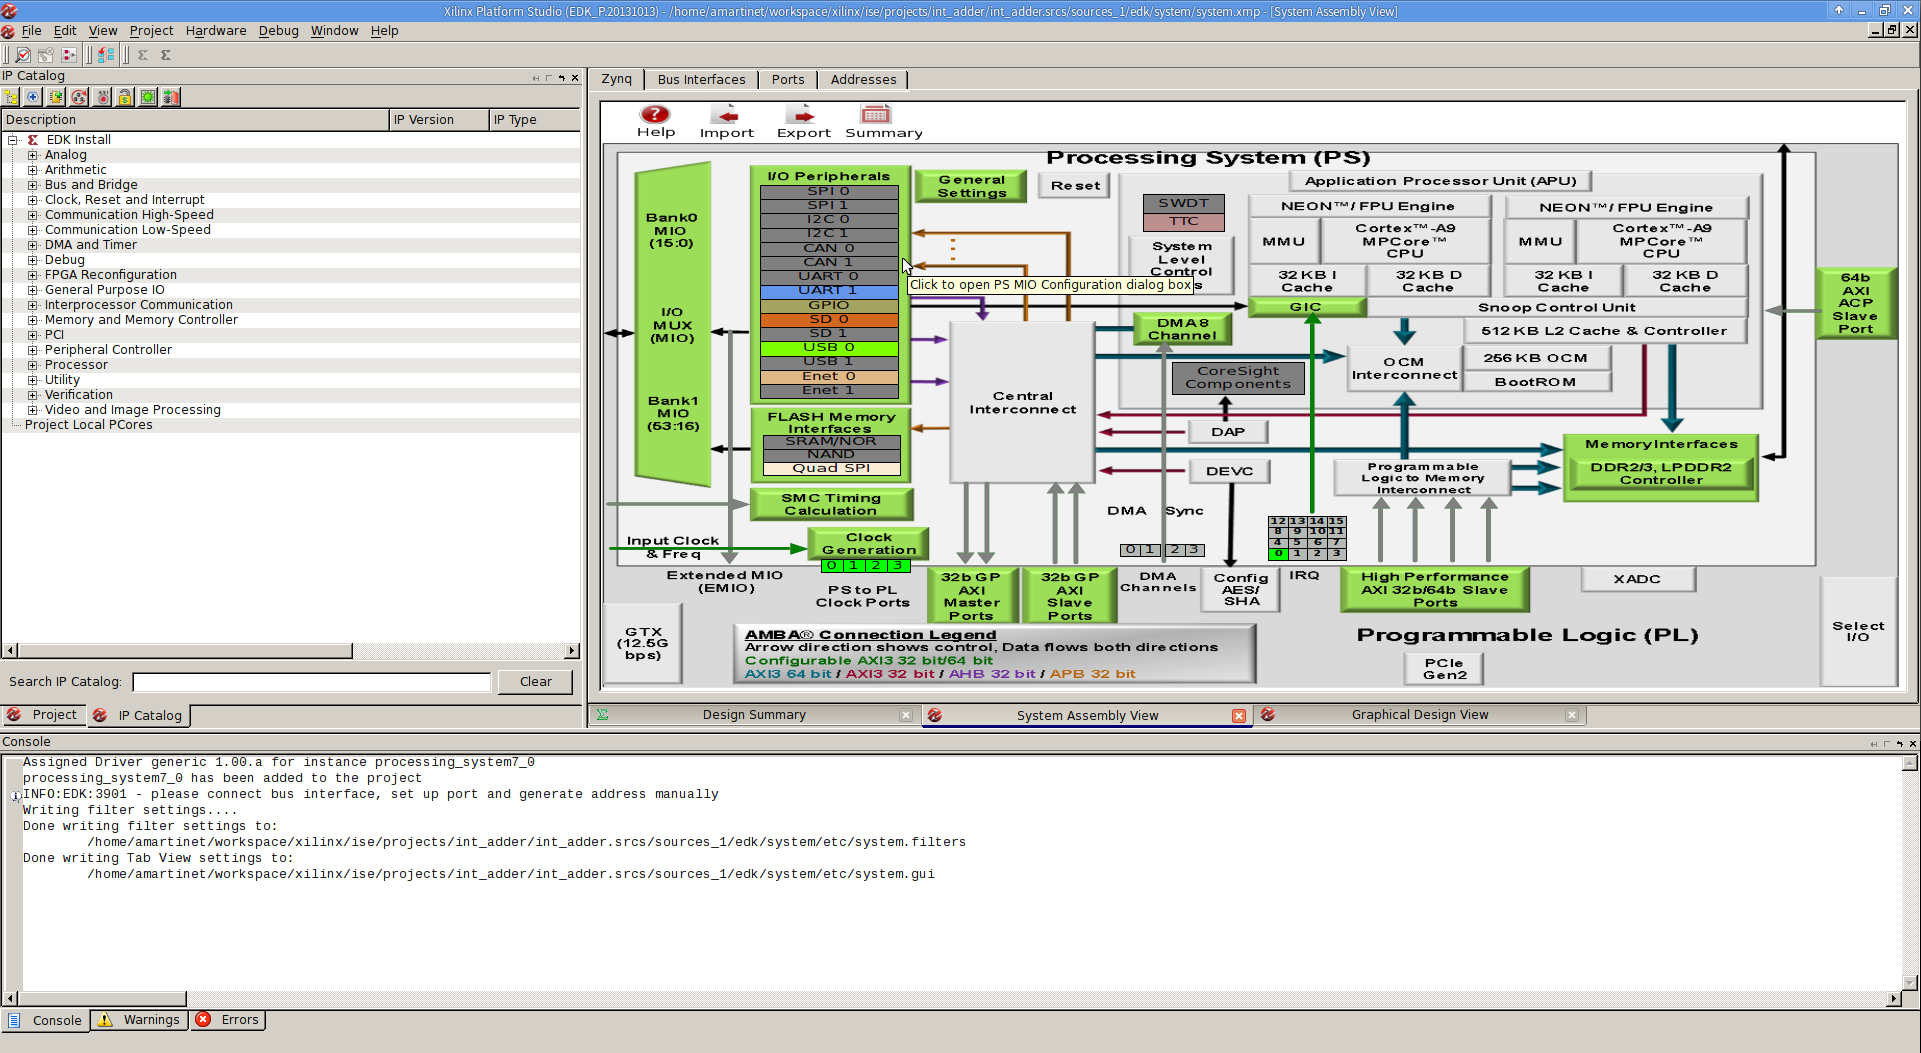
\includegraphics[scale=0.25]{pictures/MIOConfig1.png}
	\caption{MIO/GPIO Configuration}
	\end{figure}
		\item Then expand GPIO in Zynq PS Configuration Pannel.
		\item check "EMIO GPIO (with)" checkbox and set the width to 32 bits (as
				your custom peripheral has 32 bits ports)
		\item then click "Close".
	\begin{figure}
	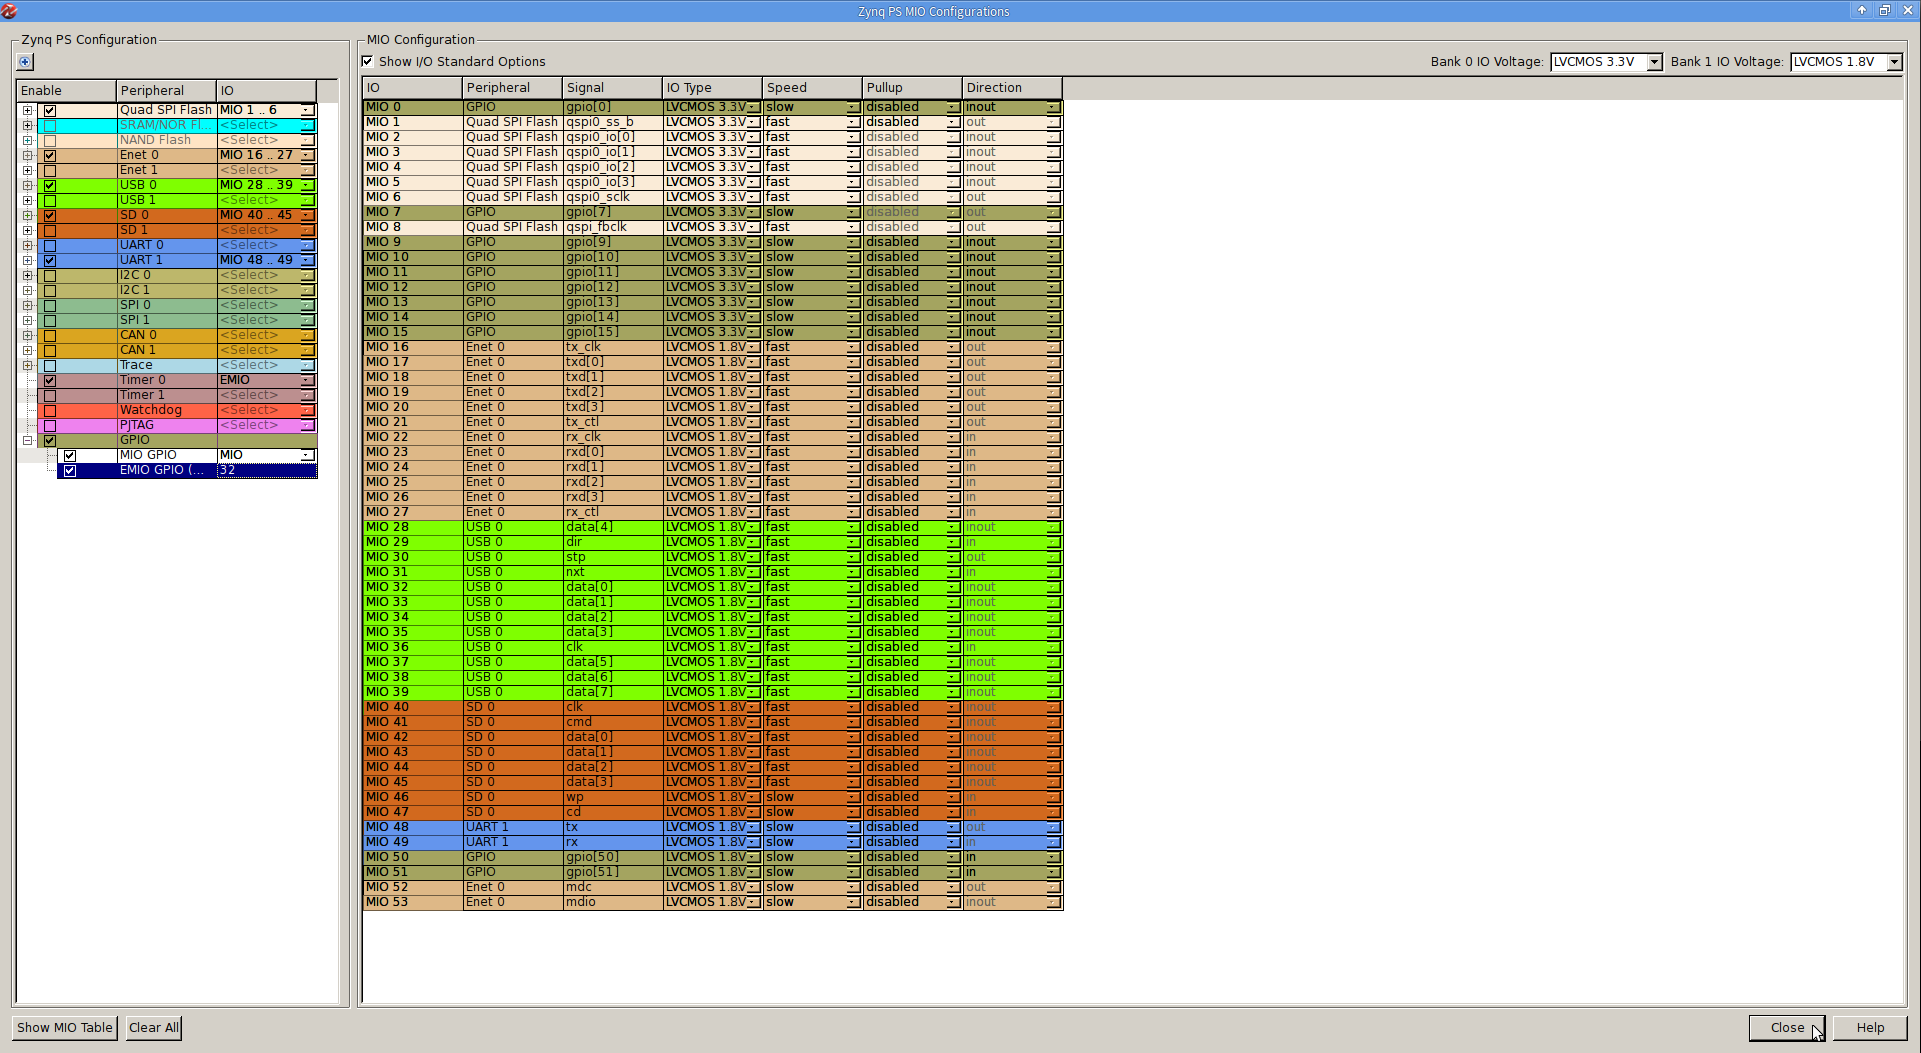
\includegraphics[scale=0.25]{pictures/MIOConfig2.png}
	\caption{Import Configuration}
	\end{figure}
	\end{itemize}

	\item Back to main XPS window, here you can already do a design rule check to see if everything is fine
	before breaking all the configuration. Go to the "Project" menu and click
	"Design rule check". You should have no warning, no error.
	\item Go to menu "Hardware" -> "Create or Import Peripheral".
	\item Getting in the wizard, click "Next" (there is nothing of interest on the
			first page).
	\begin{figure}
	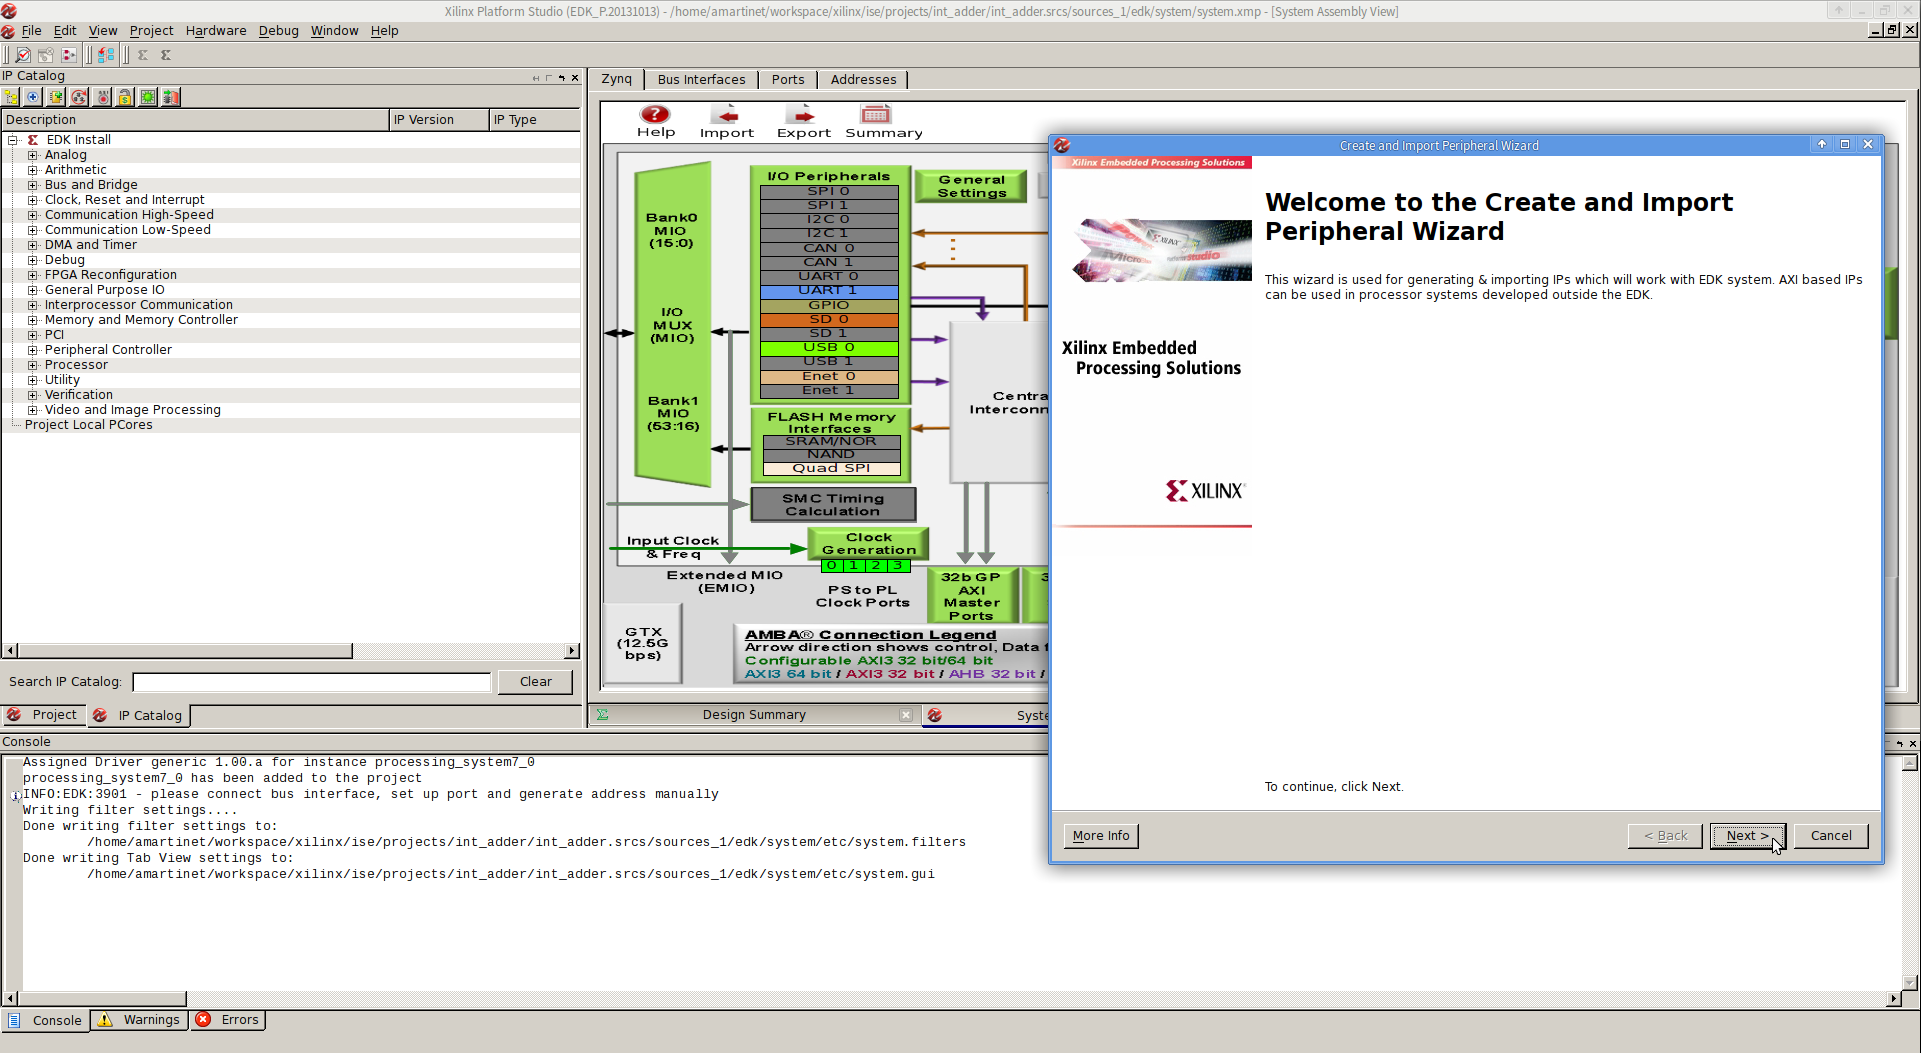
\includegraphics[scale=0.25]{pictures/ImportPeripheral1.png}
	\caption{Import Peripheral}
	\end{figure}
	\item In the "Select Flow" box, select "Import existing peripheral". Click
	"Next".
	\begin{figure}
	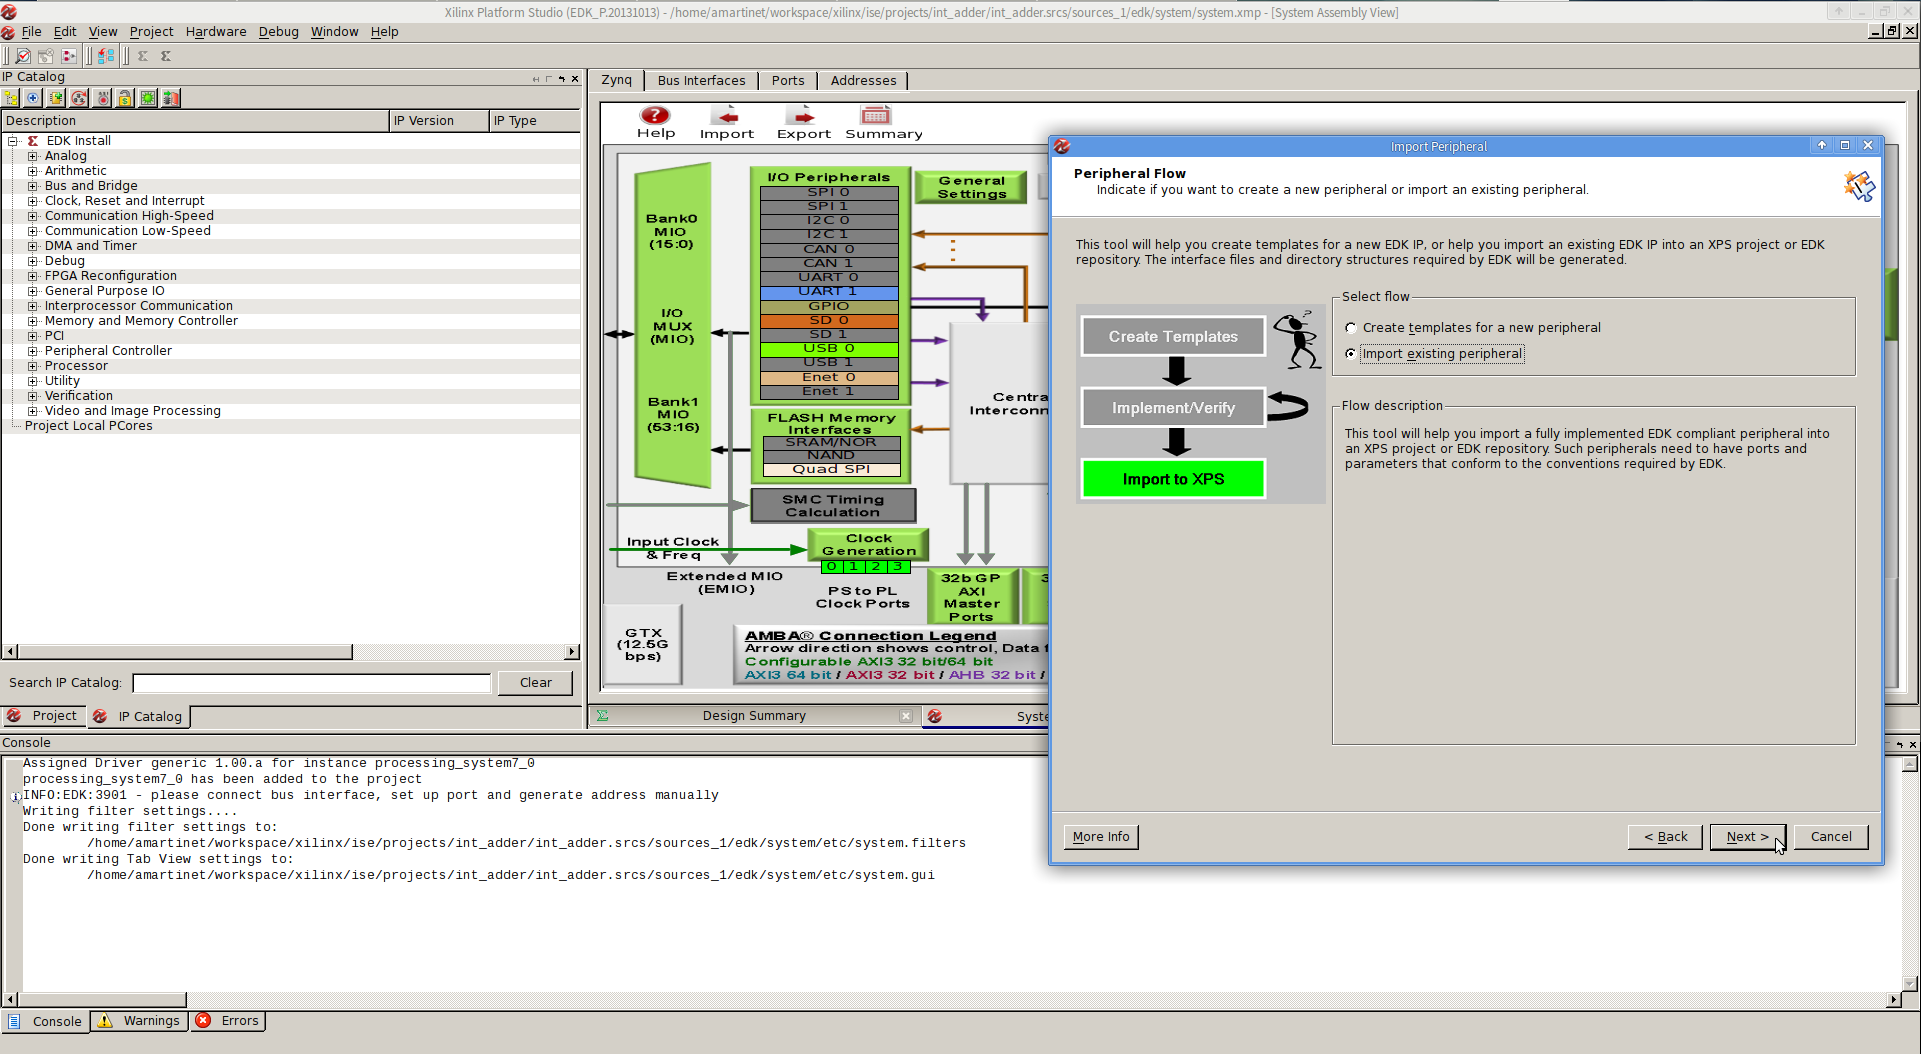
\includegraphics[scale=0.25]{pictures/ImportPeripheral2.png}
	\caption{Import Peripheral}
	\end{figure}
	\item It's important to now that SDK will copy the source file of your
	peripheral into a location before using it. Indeed, you might want to modify
	it if you did a mistake, or if you want to change some features. So you can
	modify the project file without touching to the original peripheral (that
			could be a troubling point of view, but that's not the point of the
			discussion).
	So the wizard wants to know where to store the peripheral. By default, it selects
	the current project as a repository. Leave it do it well and click "Next".
	\begin{figure}
	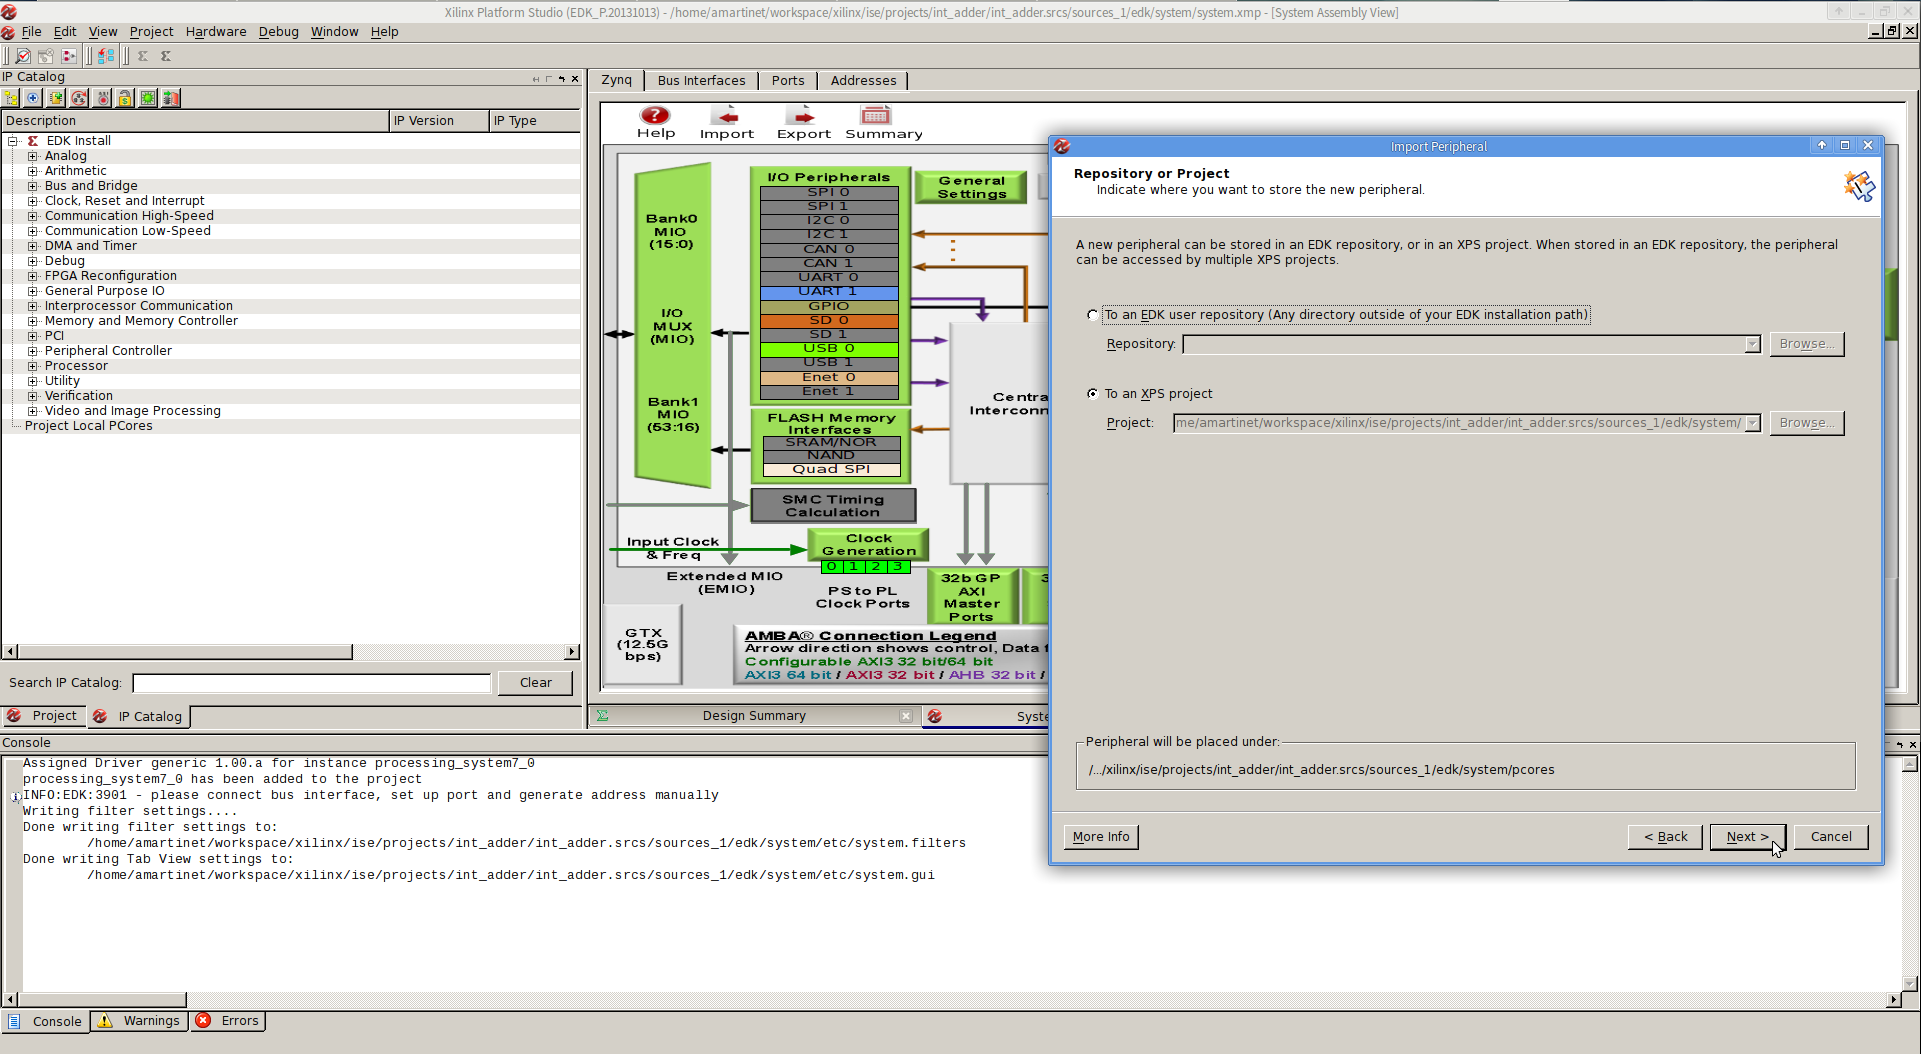
\includegraphics[scale=0.25]{pictures/ImportPeripheral3.png}
	\caption{Import Peripheral}
	\end{figure}
	\item The wizard will now ask you the name of your new peripheral. Moreover,
	it will not be able to complete the wrapper synthesis if the name of your
	peripheral doesn't match the name described in the peripheral source file,
	and won't allow you to get further than the file loading.  Fortunately, VHDL
	is non-case-sensitive, so you just have to put the flopoco-generated name
	and replace uppercase letters.  Put "intadder\_16\_f400\_uid2" as name for
	your new peripheral. The wizard provides also versionning features. Leave
	them be for the moment.  Click "Next".
	\begin{figure}
	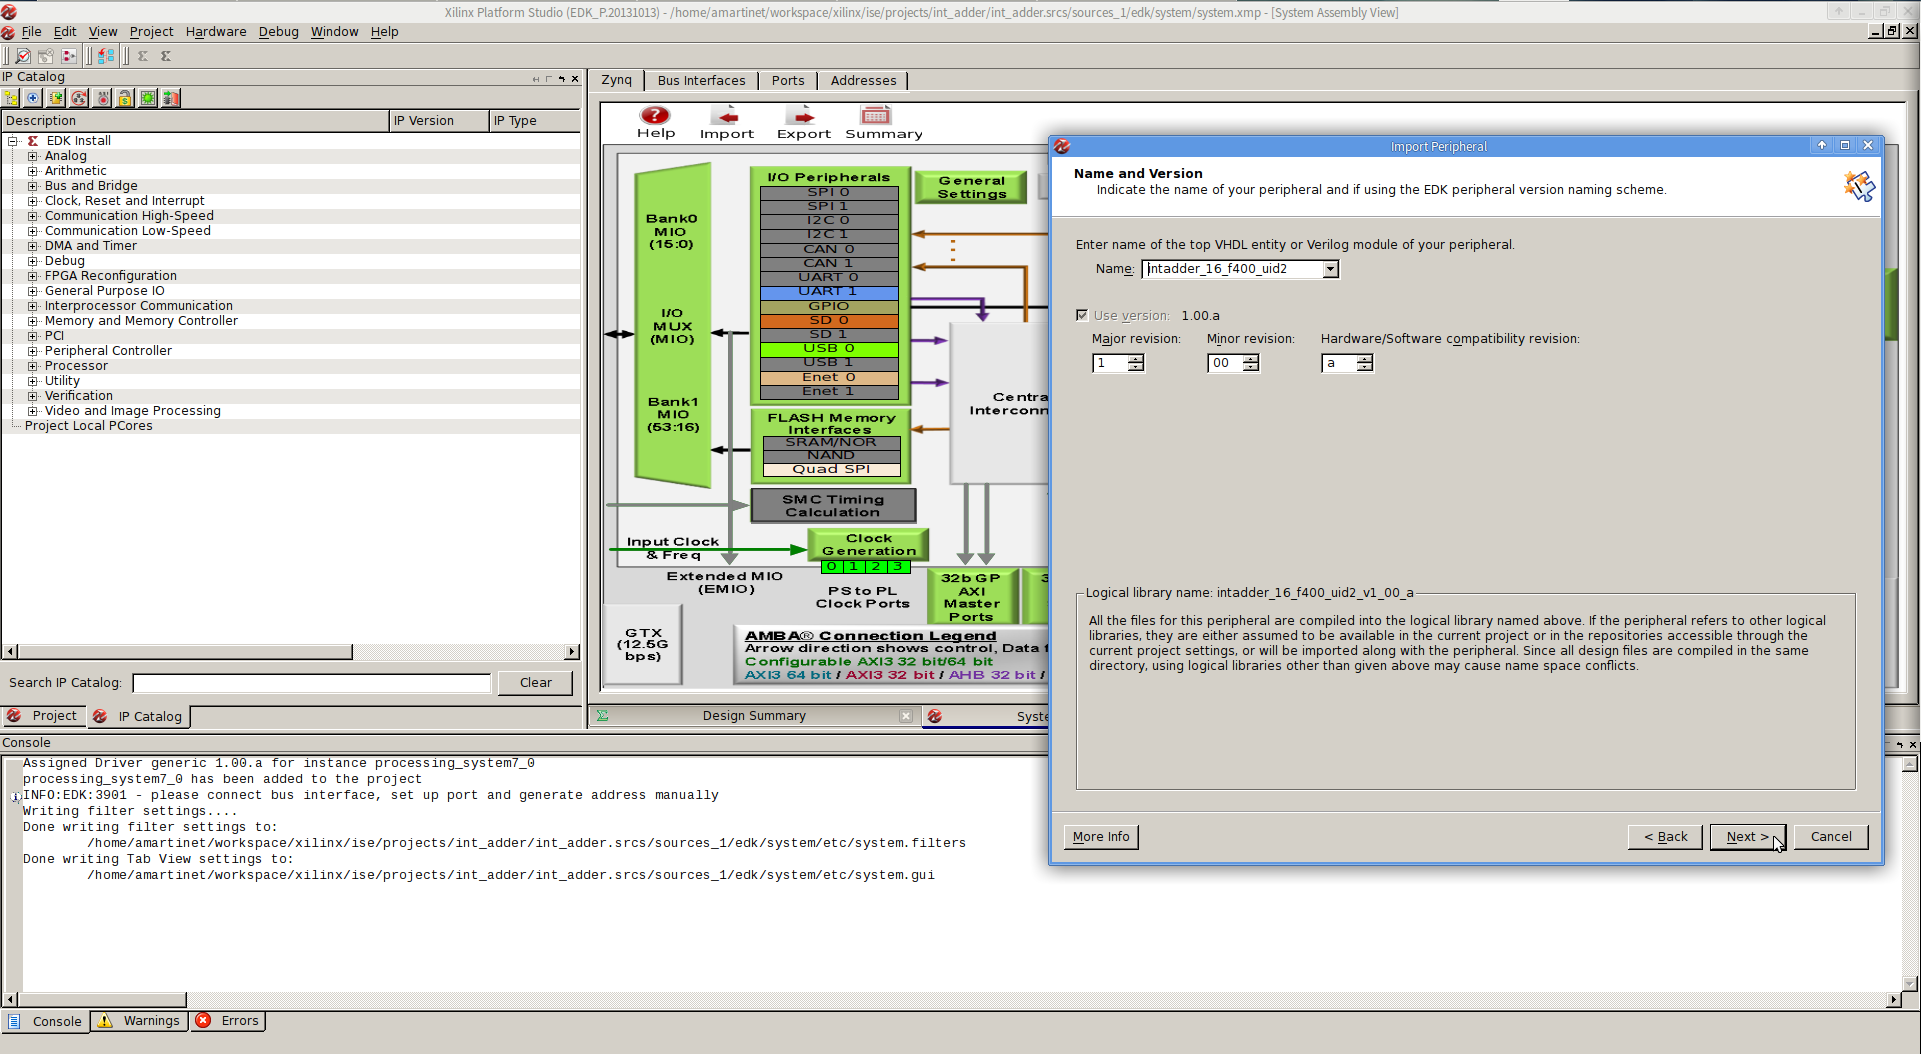
\includegraphics[scale=0.25]{pictures/ImportPeripheral4.png}
	\caption{Import Peripheral}
	\end{figure}
	\item The wizard asks now for the source file type. Leave the "HDL source
	files" checked (default) and click "Next".
	\begin{figure}
	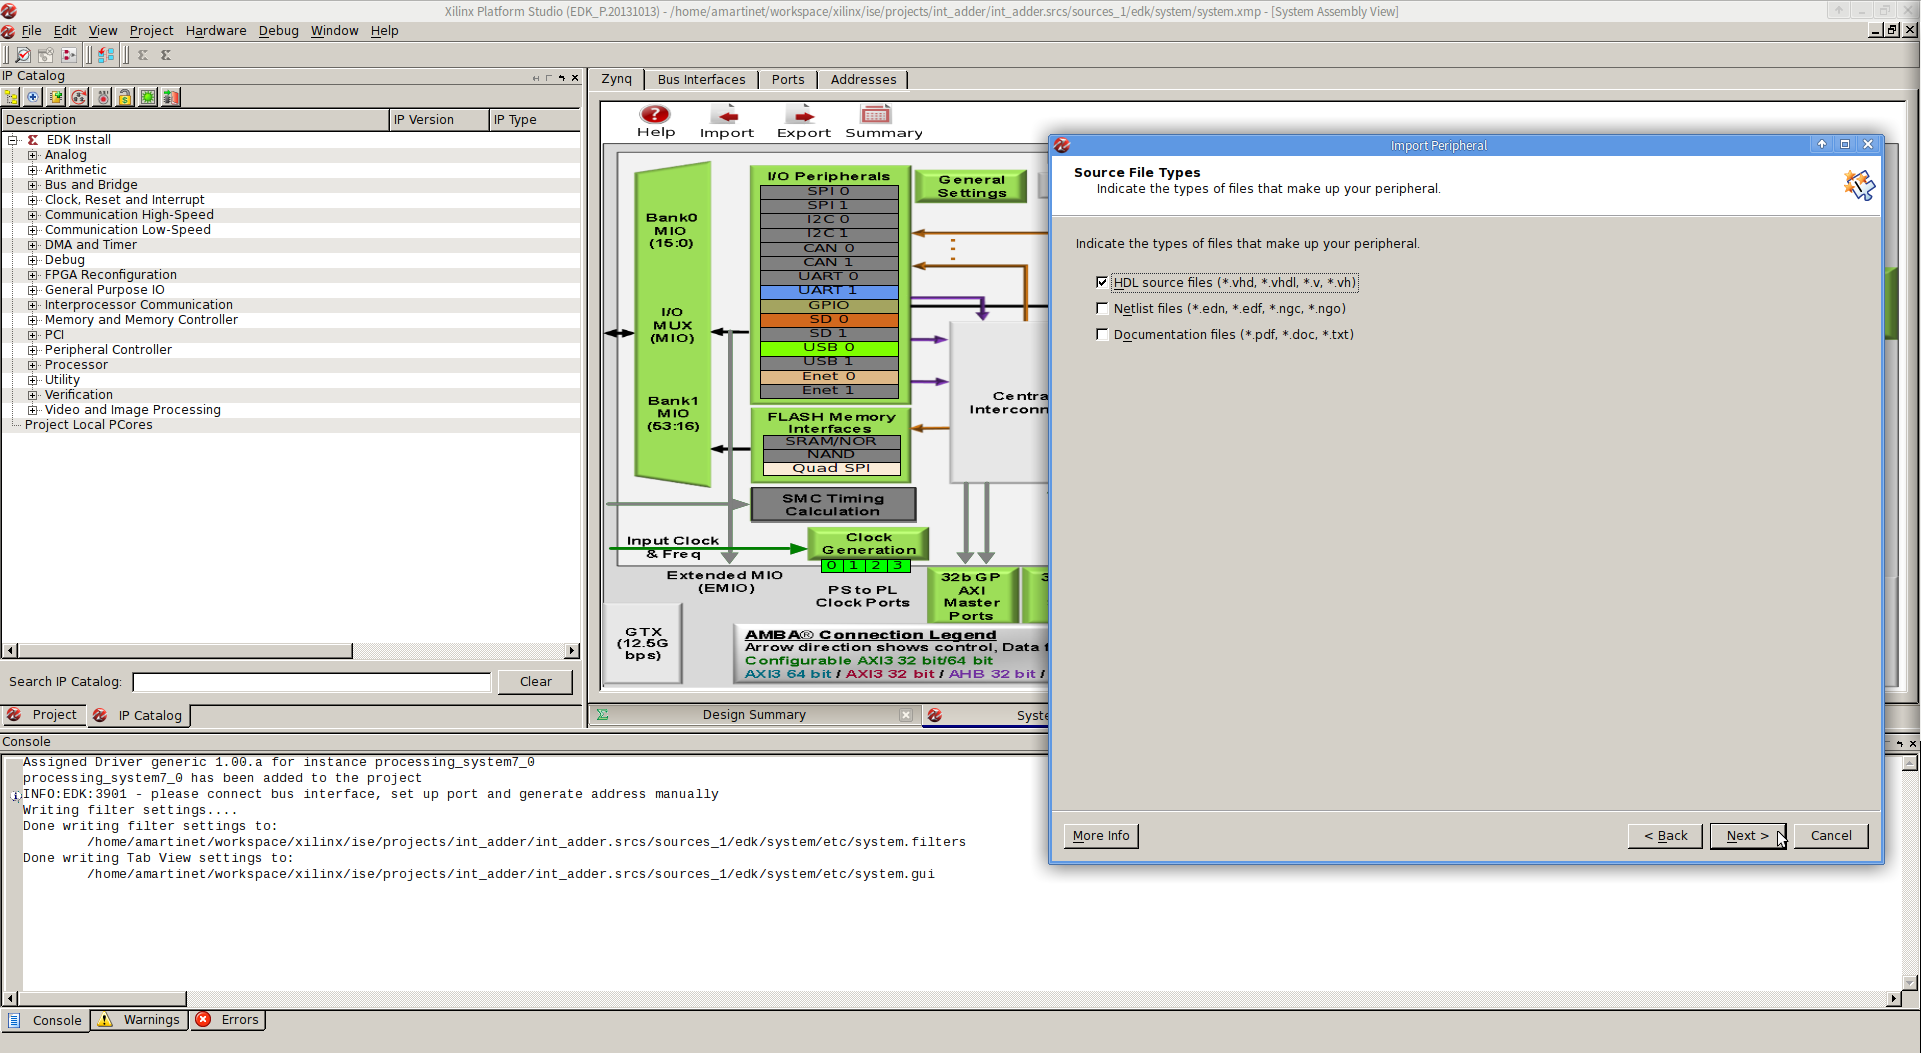
\includegraphics[scale=0.25]{pictures/ImportPeripheral5.png}
	\caption{Import Peripheral}
	\end{figure}
	\item Now specify to the wizard where to find the peripheral. Select the
	last option, "Browse to your HDL source..." and click "Next".
	\begin{figure}
	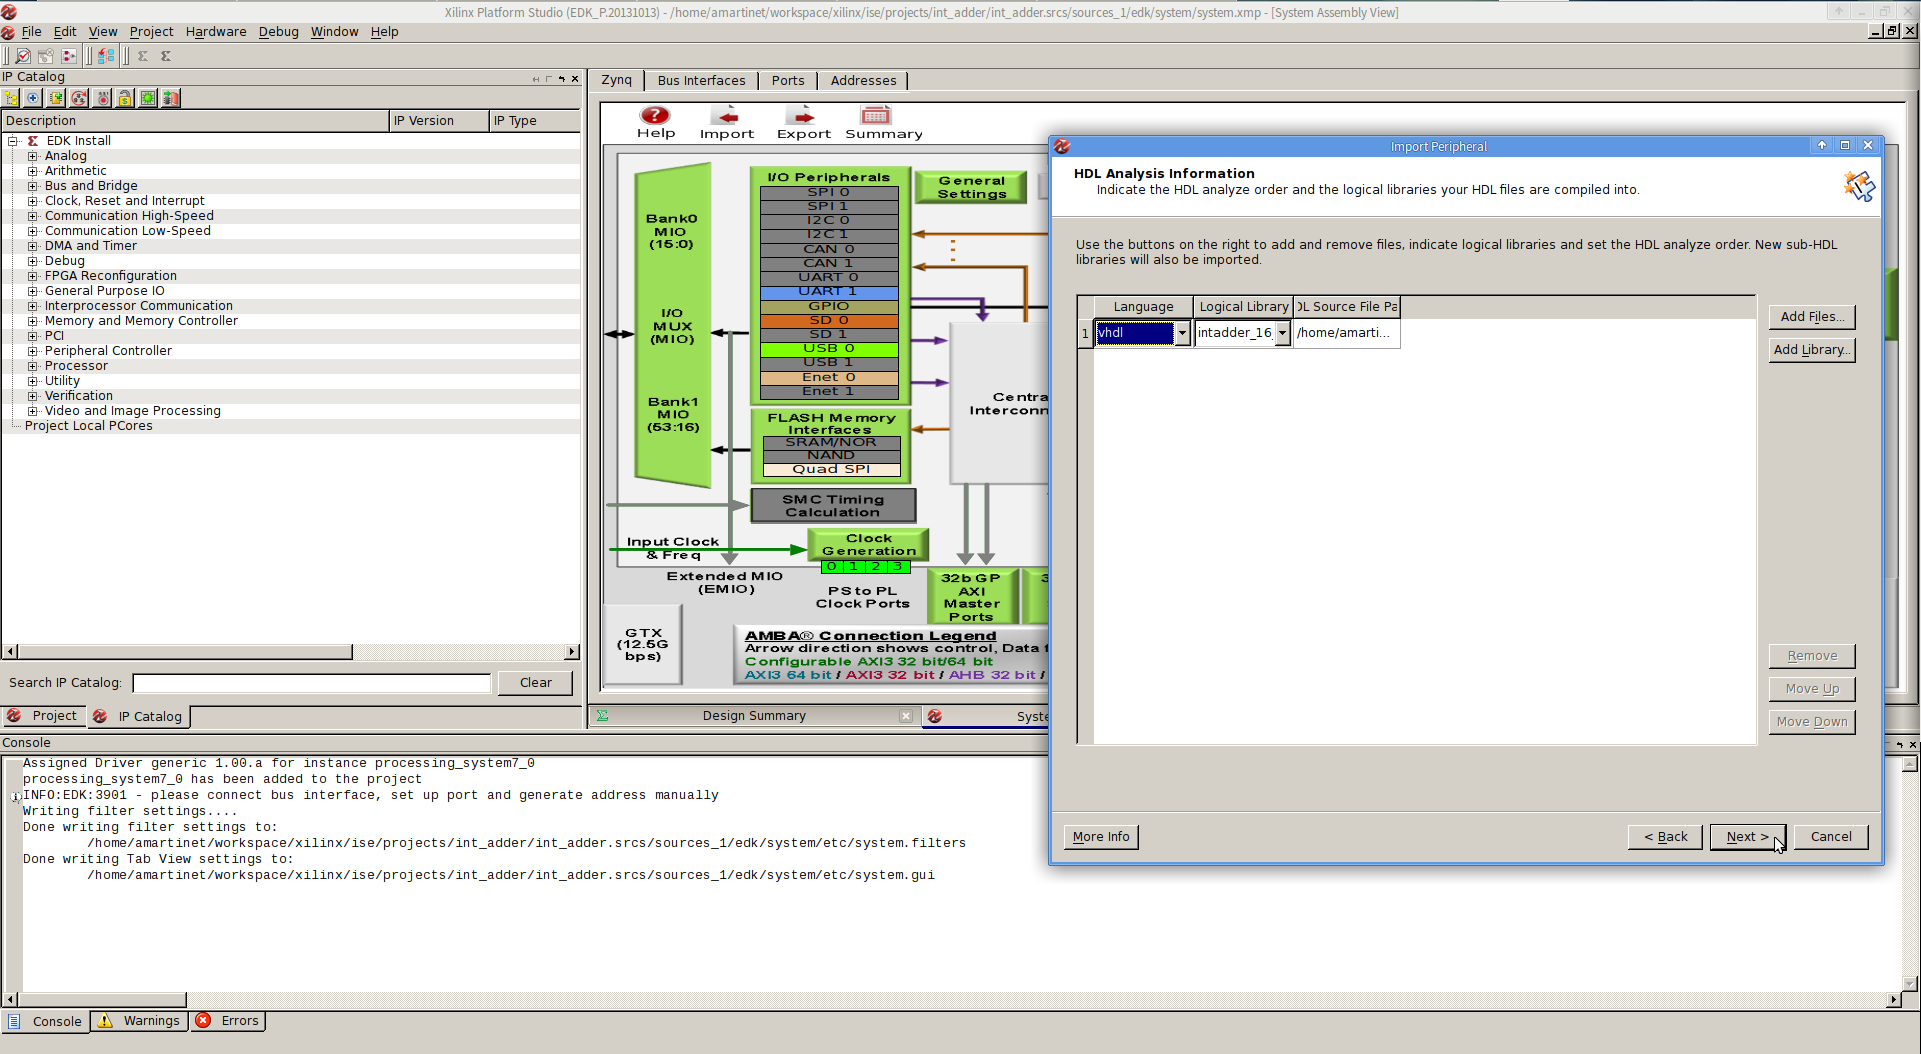
\includegraphics[scale=0.25]{pictures/ImportPeripheral7.png}
	\caption{Import Peripheral}
	\end{figure}
	\item Then click on the "Add Files" button and browse your vhdl component,
	so int\_adder\_16.vhdl. It appears as first line of the table.
	Click "Next".
	\item The wizard will tell you that it doesn't manage to find the top
	design. This seems to happen because it uses the name of the peripheral
	(library) to infer	the name of the top module. Here we've no problem,
	because we have only one	file. In case of several files, this could
	easily be worked around moving up or down top module files. Indeed, as you
	can see it takes the first file of the list as top design file.
	Click "OK".
	\begin{figure}
	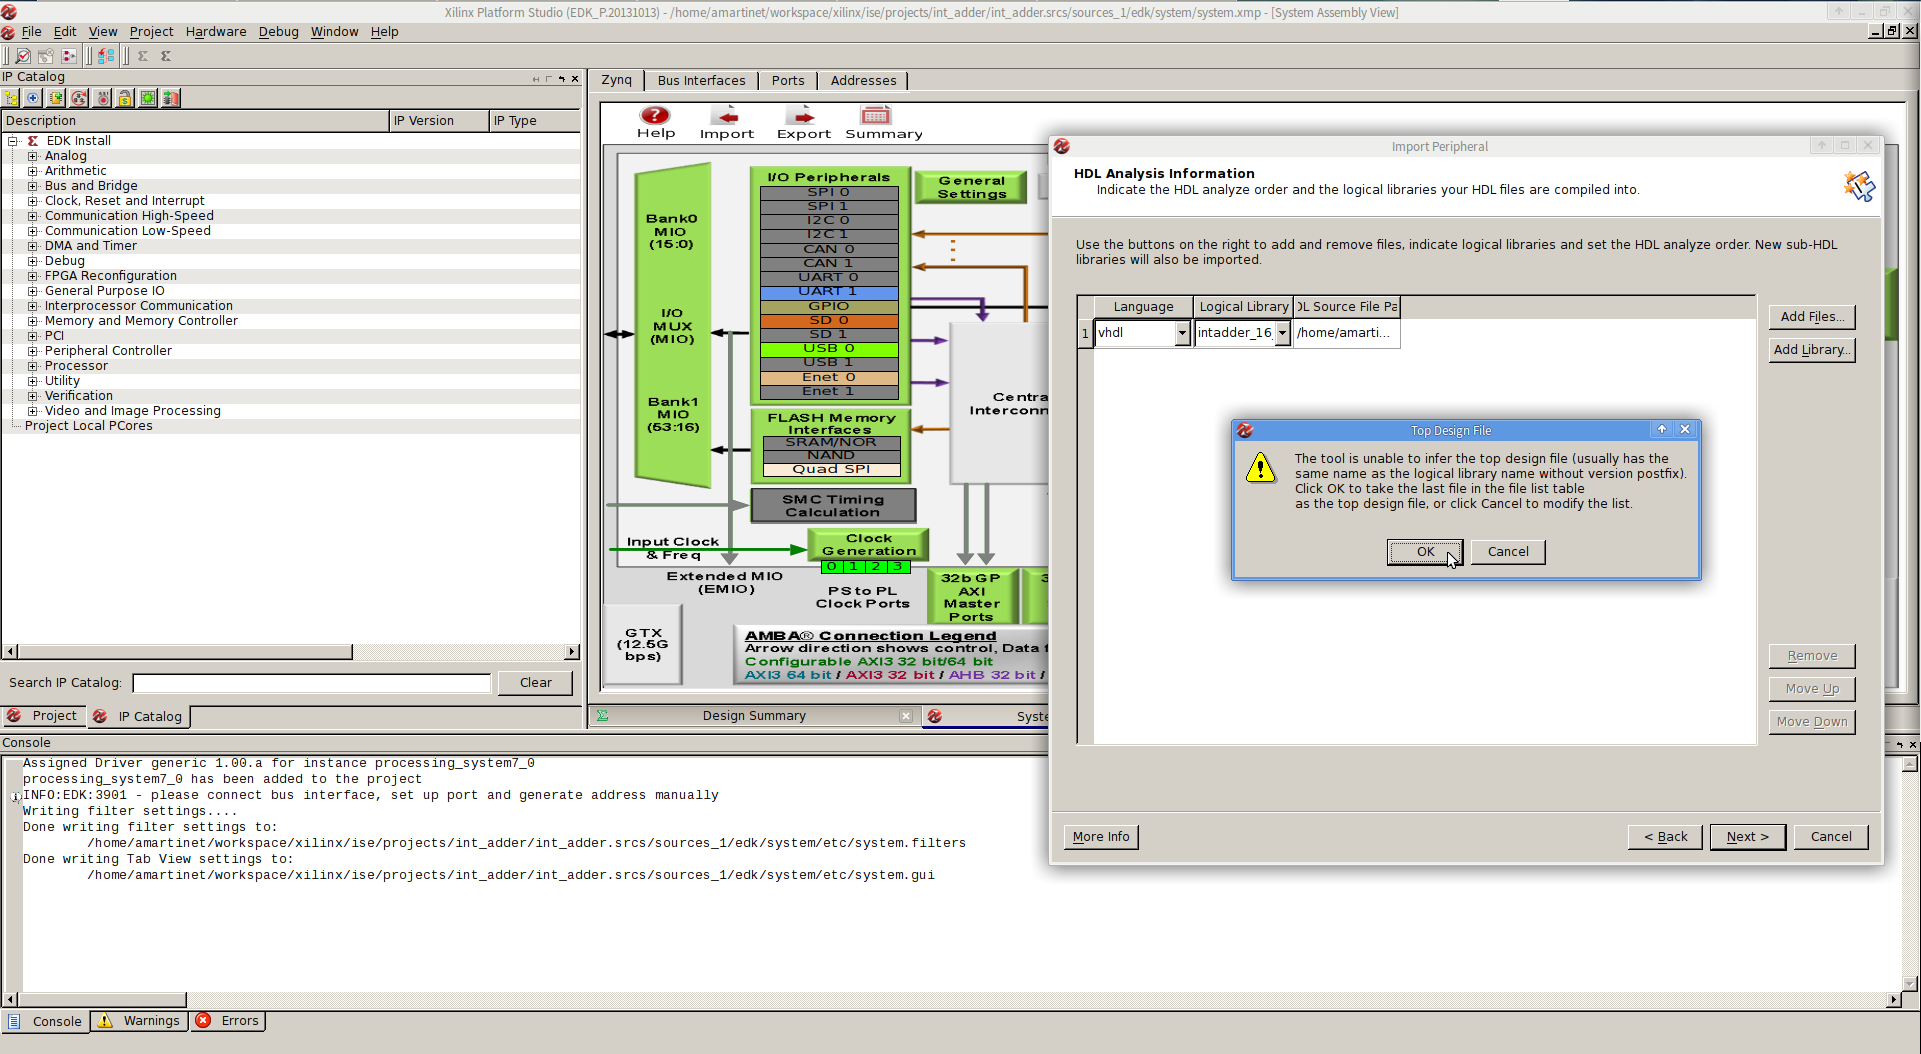
\includegraphics[scale=0.25]{pictures/ImportPeripheral8.png}
	\caption{Import Peripheral}
	\end{figure}
	\item Now you're going to specify bus interfaces compatibilities.
	As flopoco's int\_adder\_16 doesn't follow any standard protocol (we don't
			need it for a simple adder), uncheck the main "Select bu
	interface(s)" box. Click "Next".
	\begin{figure}
	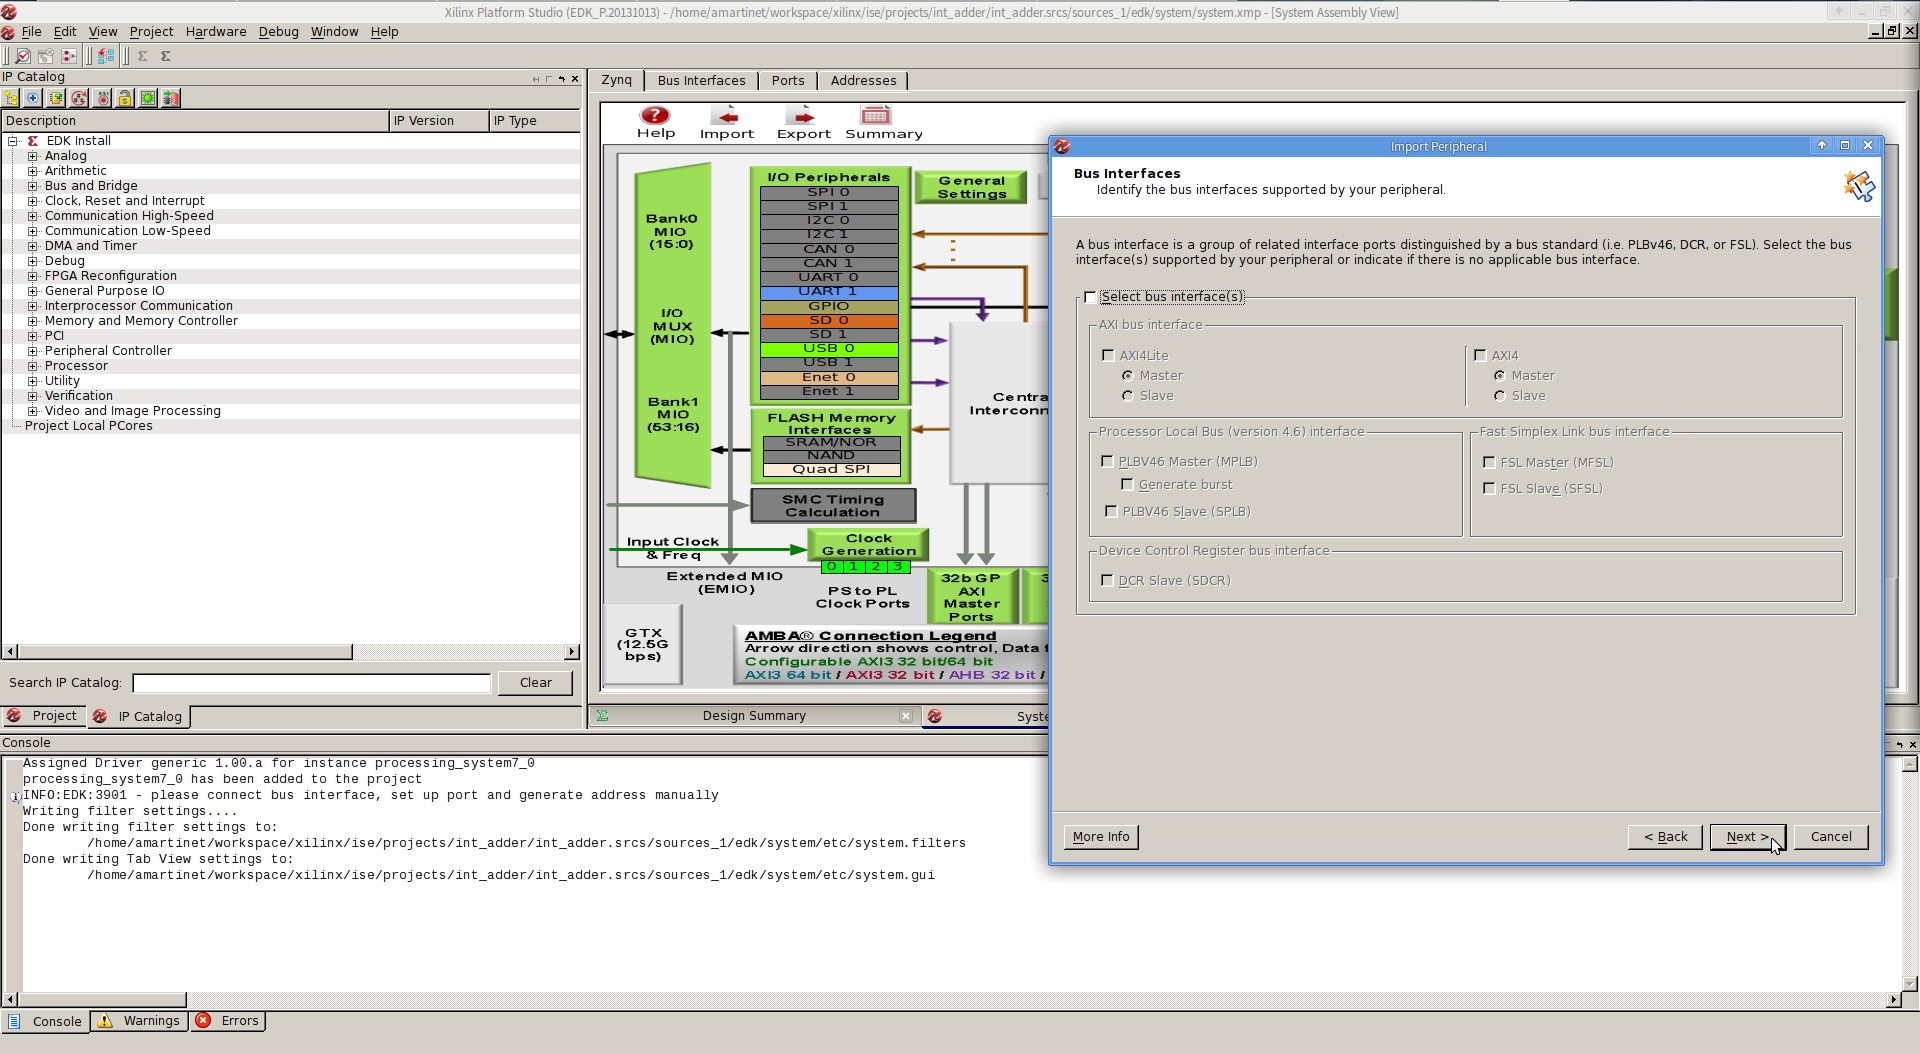
\includegraphics[scale=0.25]{pictures/ImportPeripheral9.png}
	\caption{Import Peripheral}
	\end{figure}
	\item Now the wizard wants to know if your peripheral generates interrupts.
	Actually it doesn't, so uncheck "Select and configure interrupt(s)" box.
	Click "Next".
	\begin{figure}
	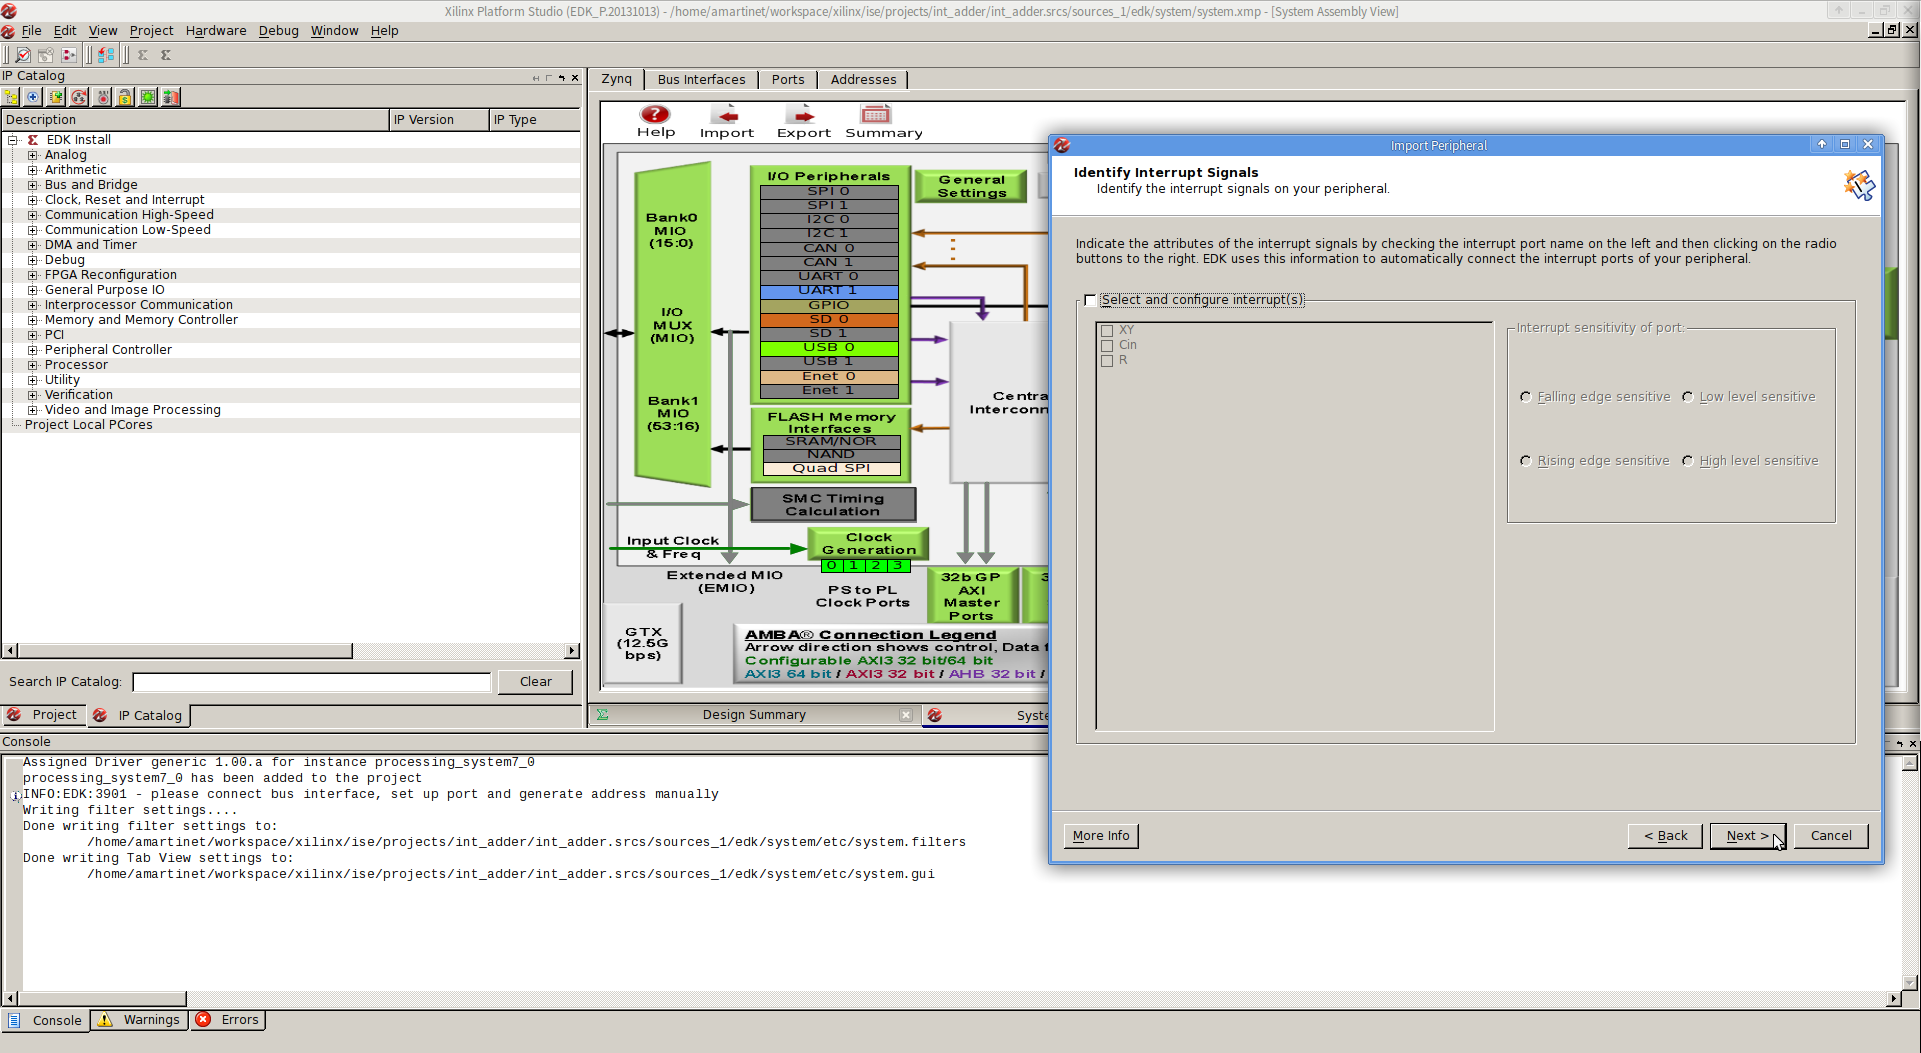
\includegraphics[scale=0.25]{pictures/ImportPeripheralA.png}
	\caption{Import Peripheral}
	\end{figure}
	\item Then you can predefine where ports will be connected. This could be
	interesting when you use clock, reset pins, and some common standard
	features, which may not be automatically detected. As we don't follow any standard protocol, we are going to plug the
	peripheral manually. Leave everything be and click "Next".
	\begin{figure}
	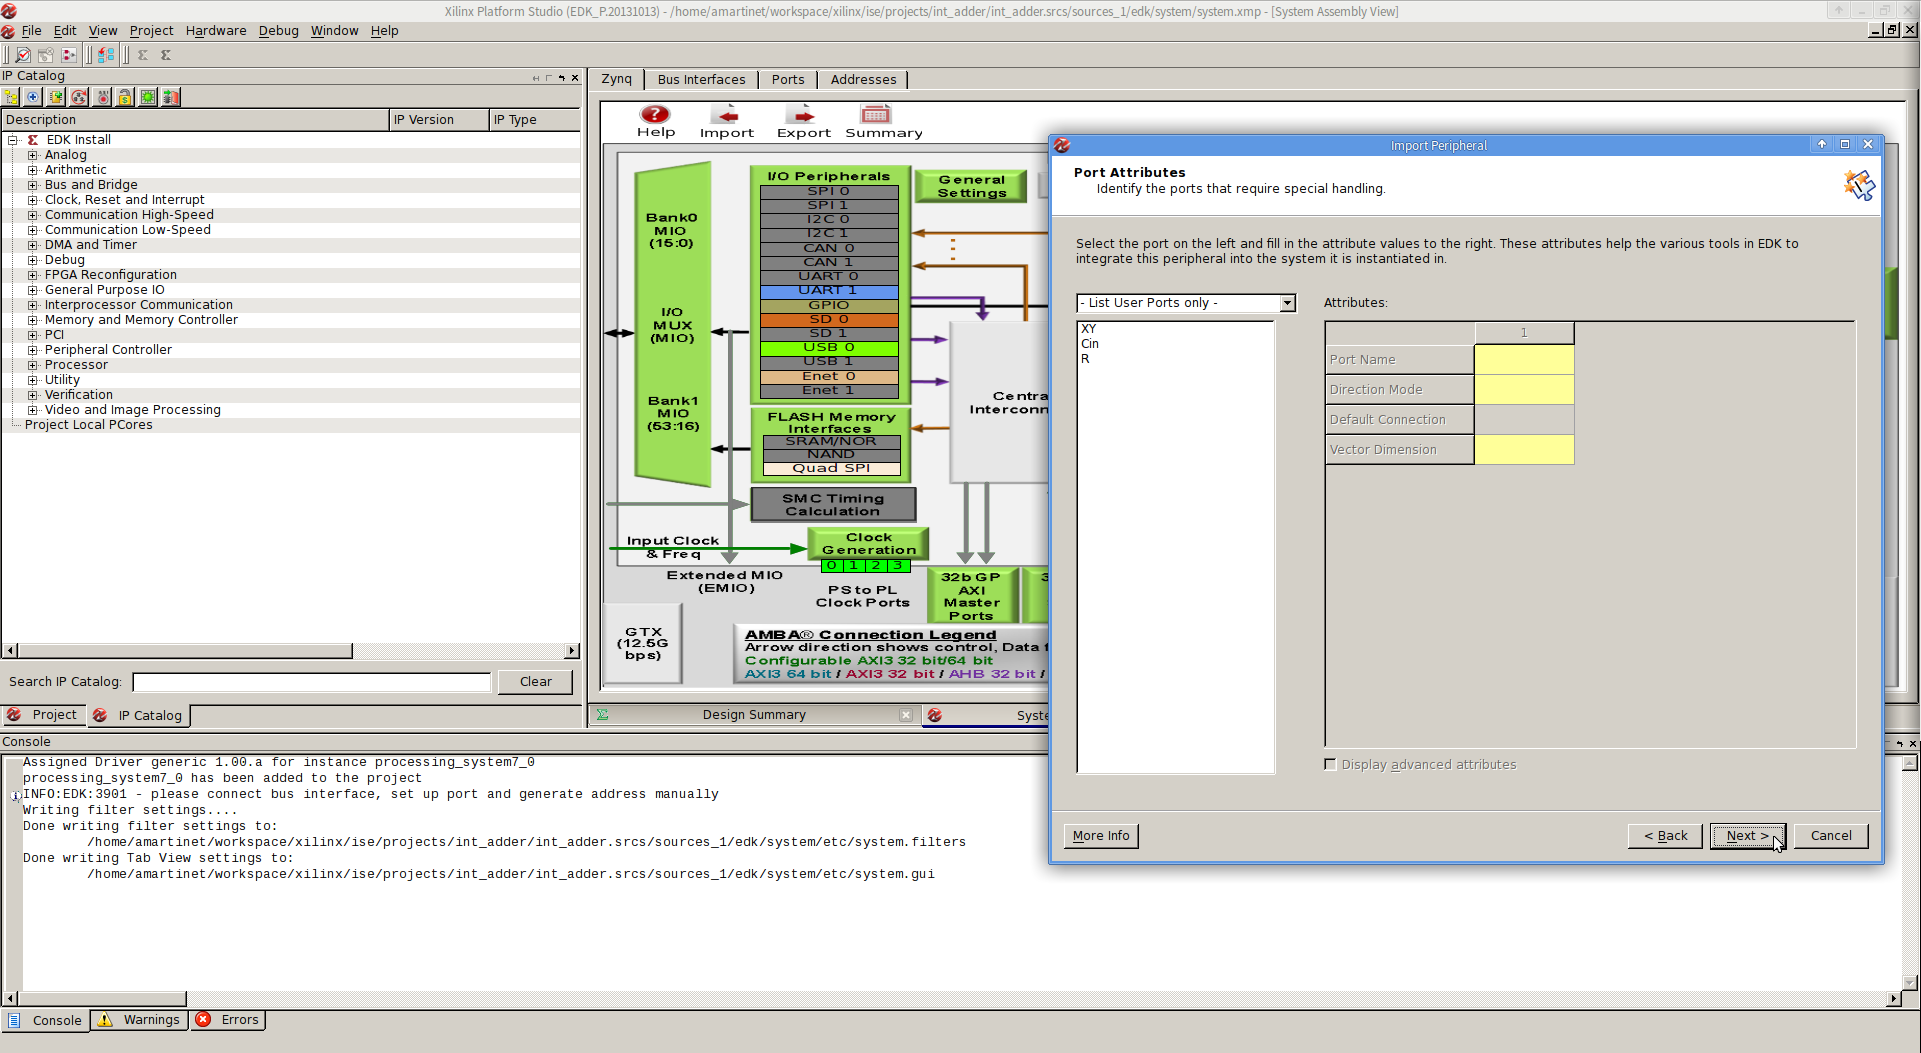
\includegraphics[scale=0.25]{pictures/ImportPeripheralB.png}
	\caption{Import Peripheral}
	\end{figure}
	\item Now you get into the last summary page when you can check if the
	wizard well understood what the hell you are doing. Click "Finish" to create
	your peripheral or get back to the previous steps if you feel unsatisfied.
	Wait for the GUI to entire rebuild itself.
	\begin{figure}
	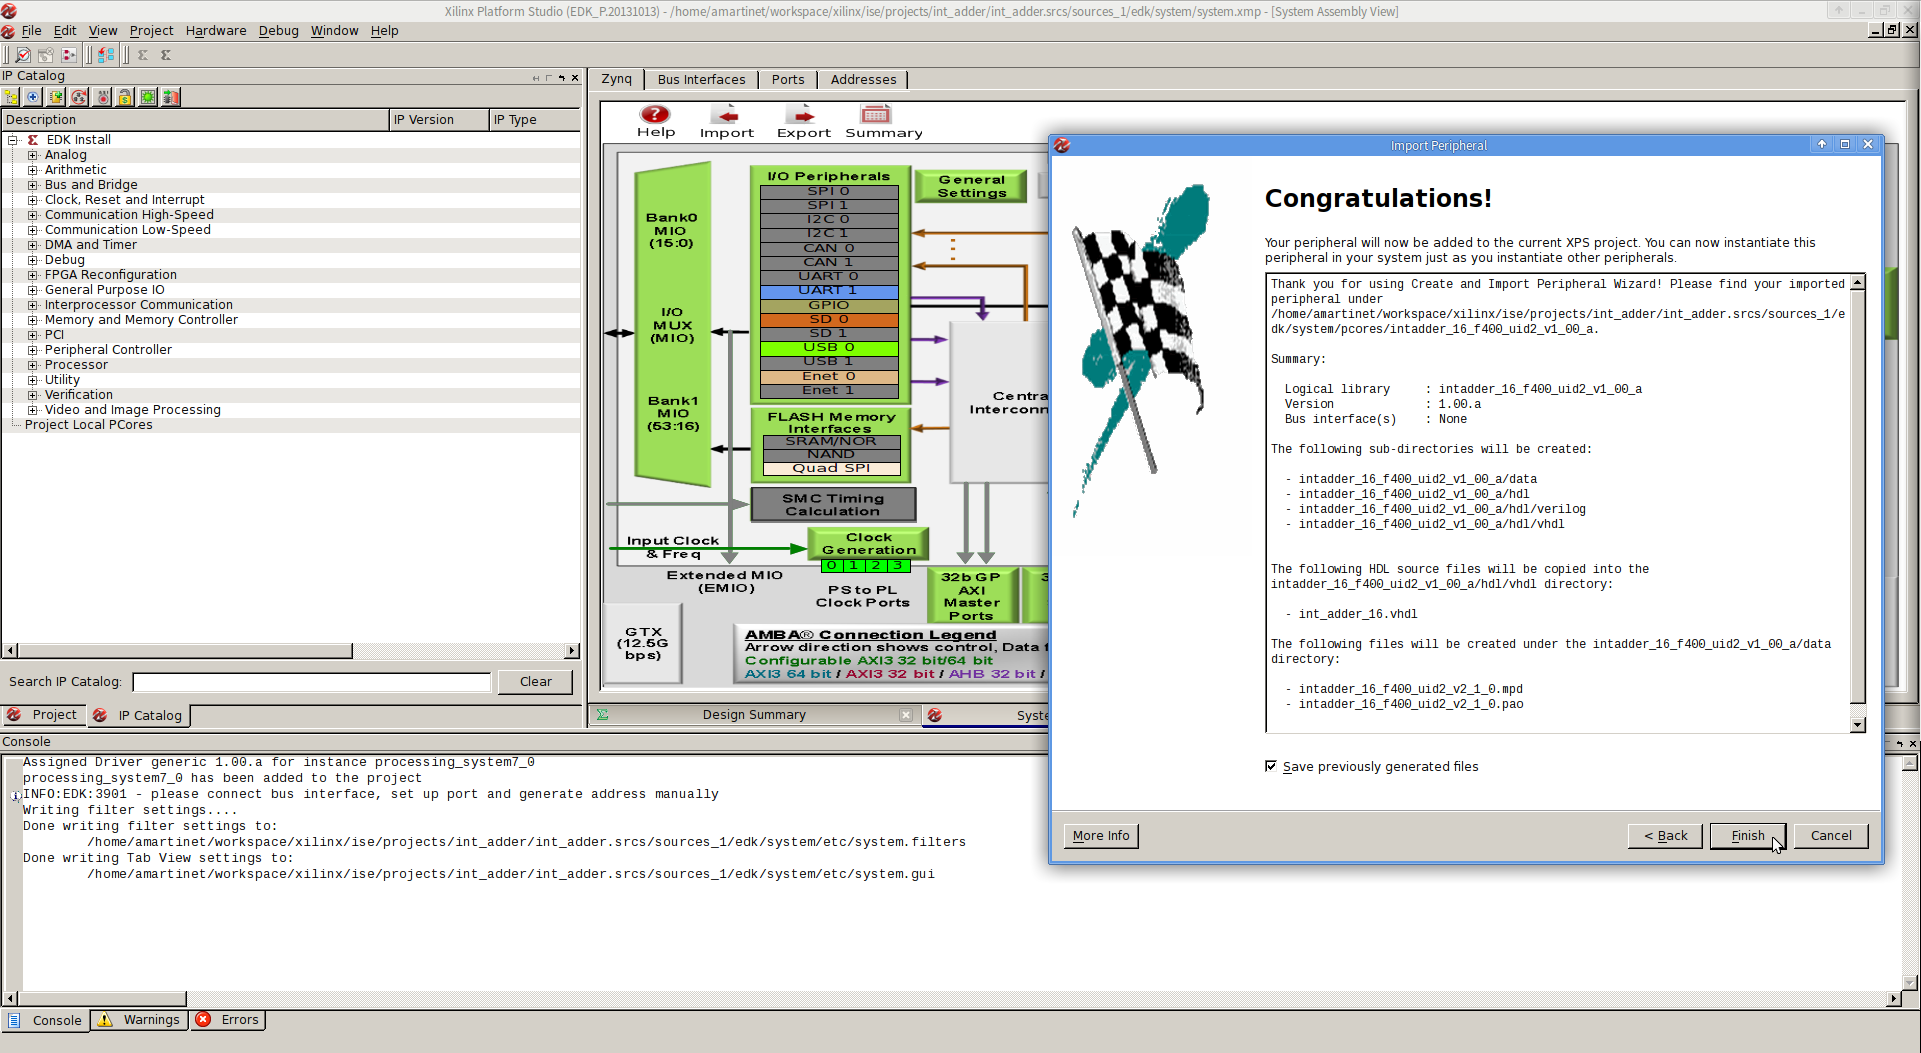
\includegraphics[scale=0.25]{pictures/ImportPeripheralC.png}
	\caption{Import Peripheral}
	\end{figure}
	\item You will see that a new field "USER" appeared in the "IP Catalog" Pannel.
	Expand it and double click your new peripheral to add it to the hardware
	design. Click "Yes" to the confirmation message. Then Click "OK" in the "Core
	Config" window that poped up.
	\begin{figure}
	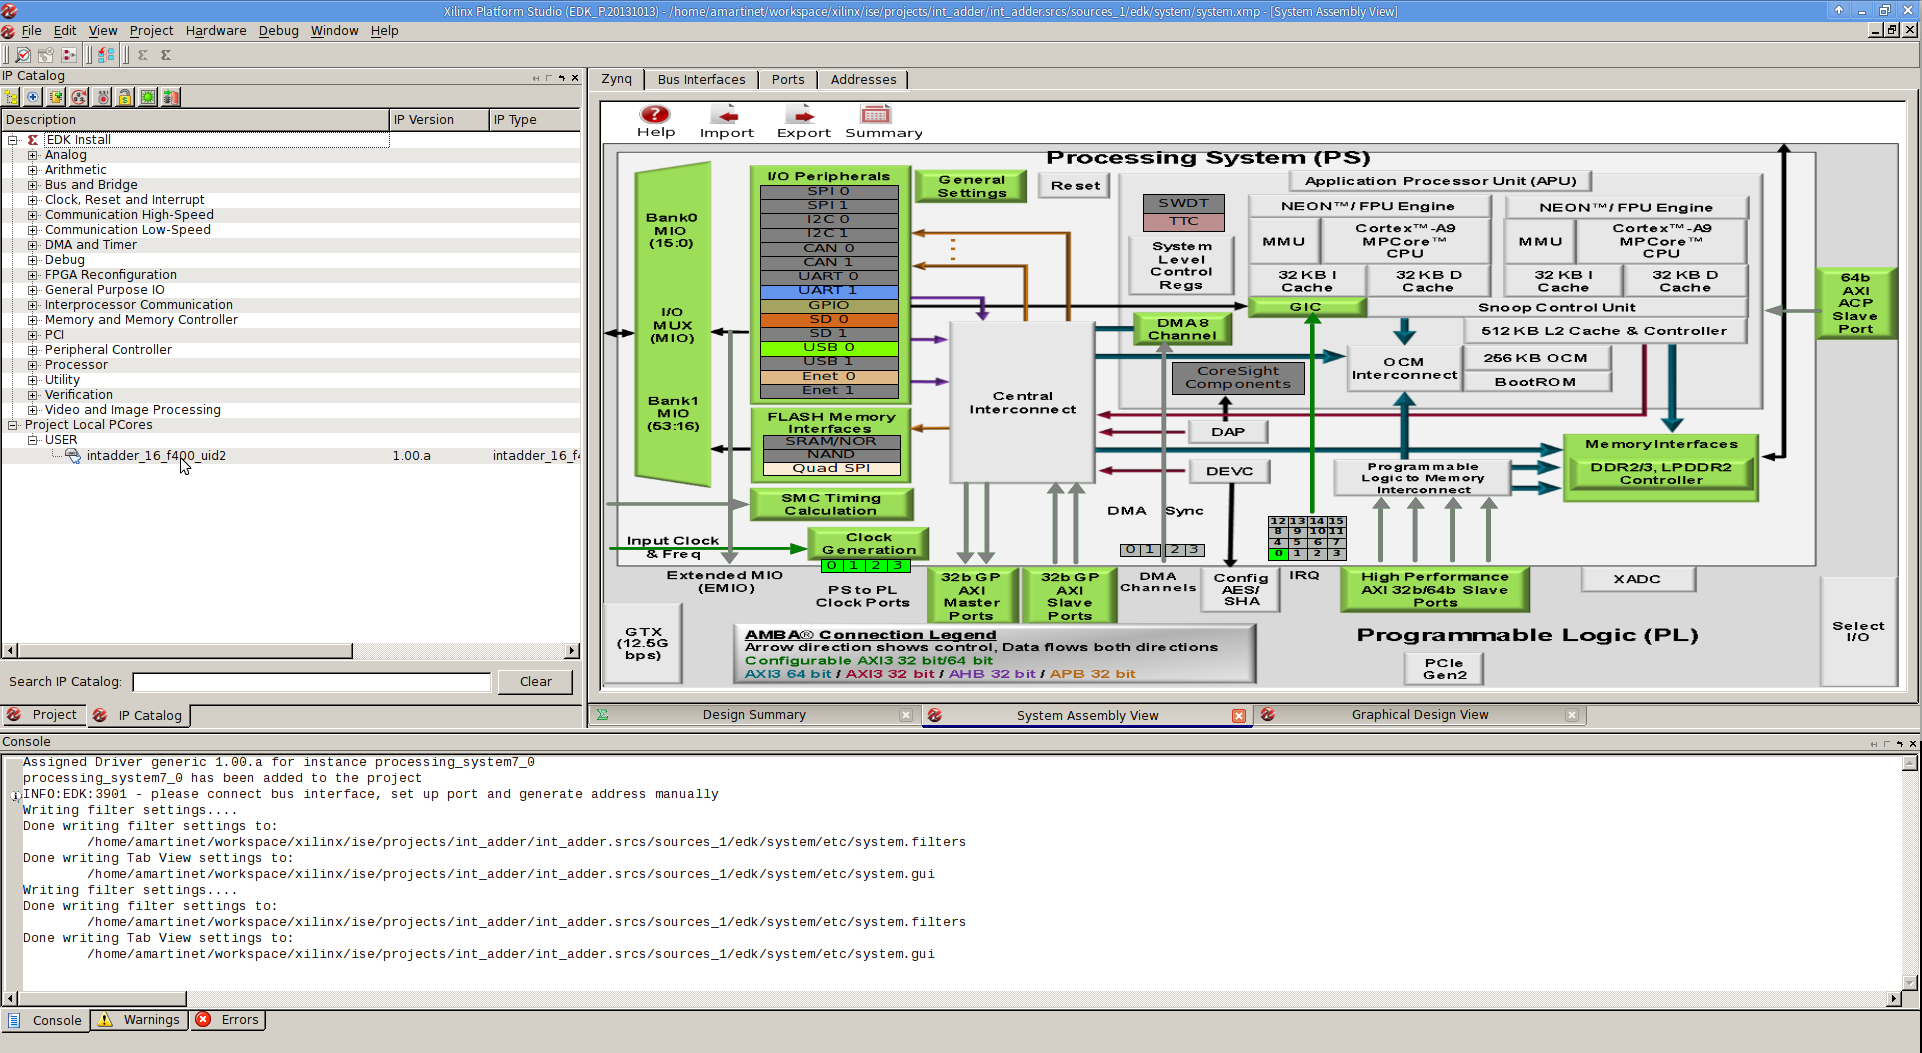
\includegraphics[scale=0.25]{pictures/AddPeripheral1.png}
	\caption{Add custom IP}
	\end{figure}
	\begin{figure}
	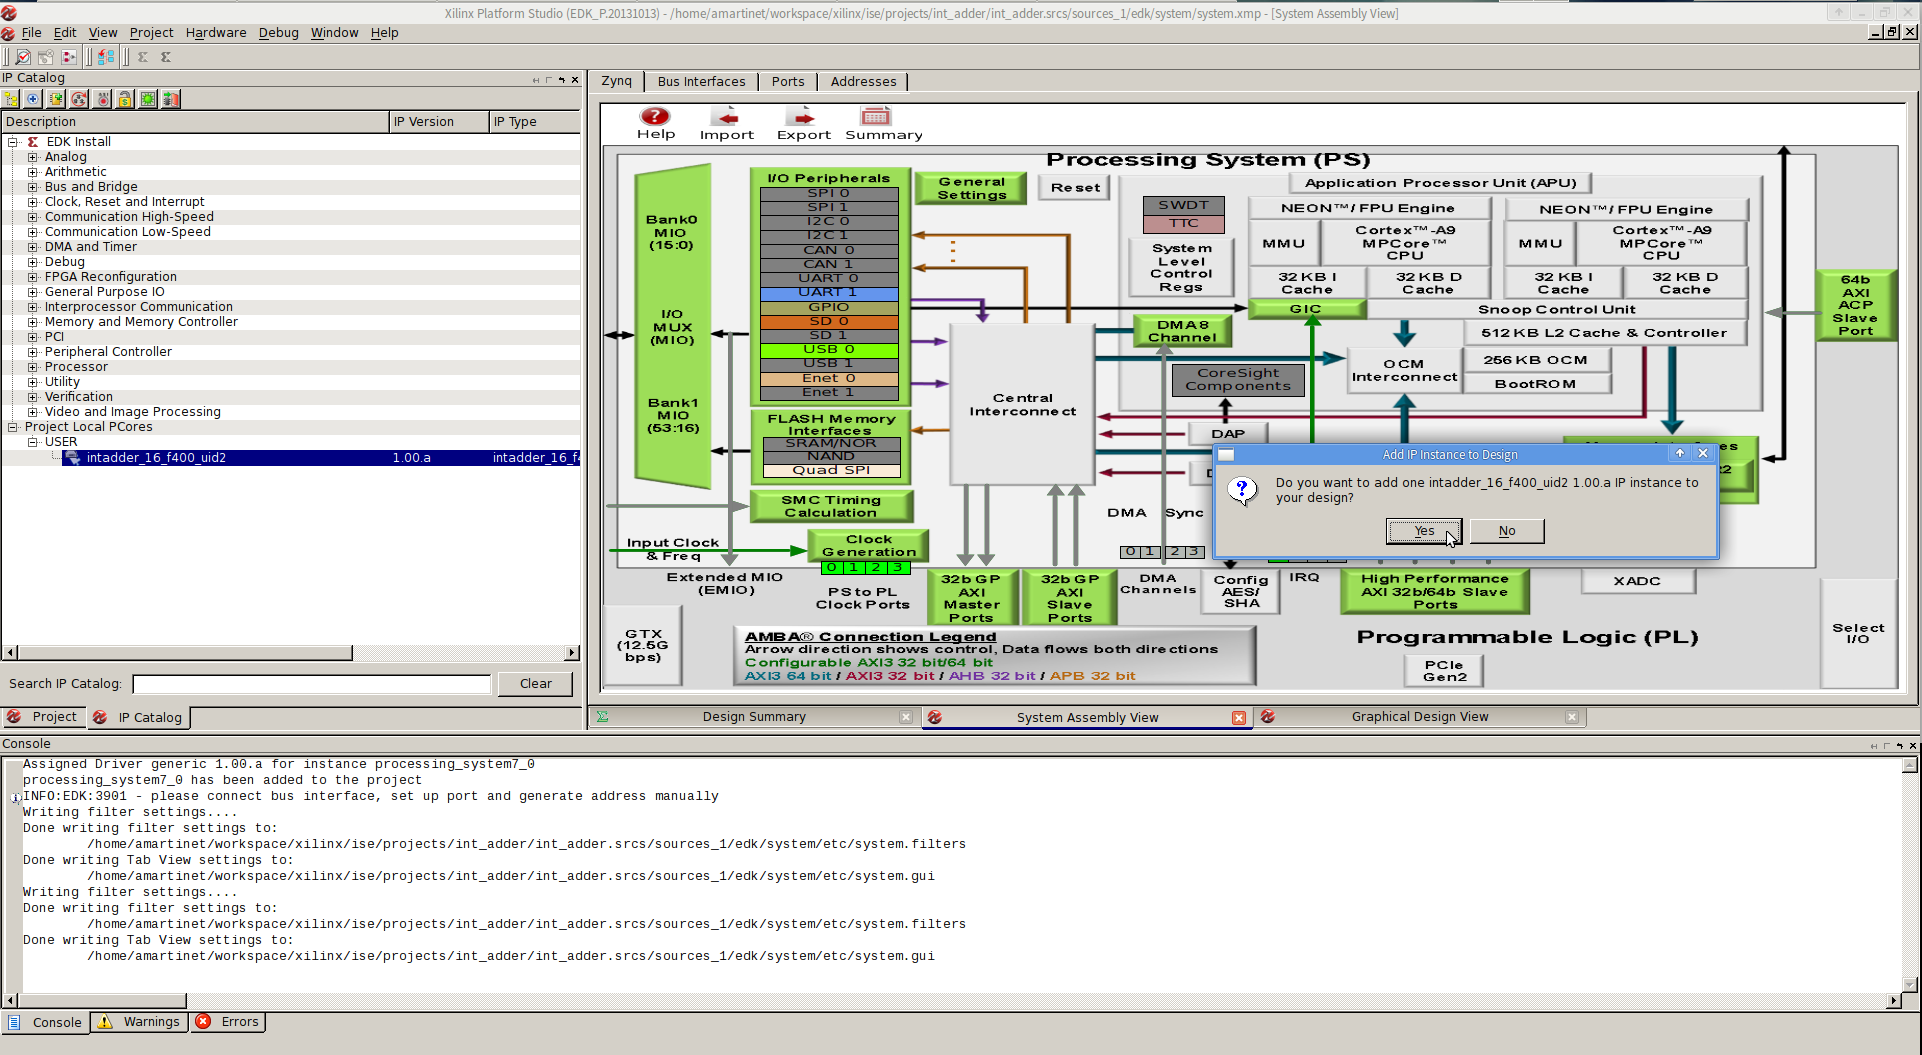
\includegraphics[scale=0.25]{pictures/AddPeripheral2.png}
	\caption{Add custom IP}
	\end{figure}
	\begin{figure}
	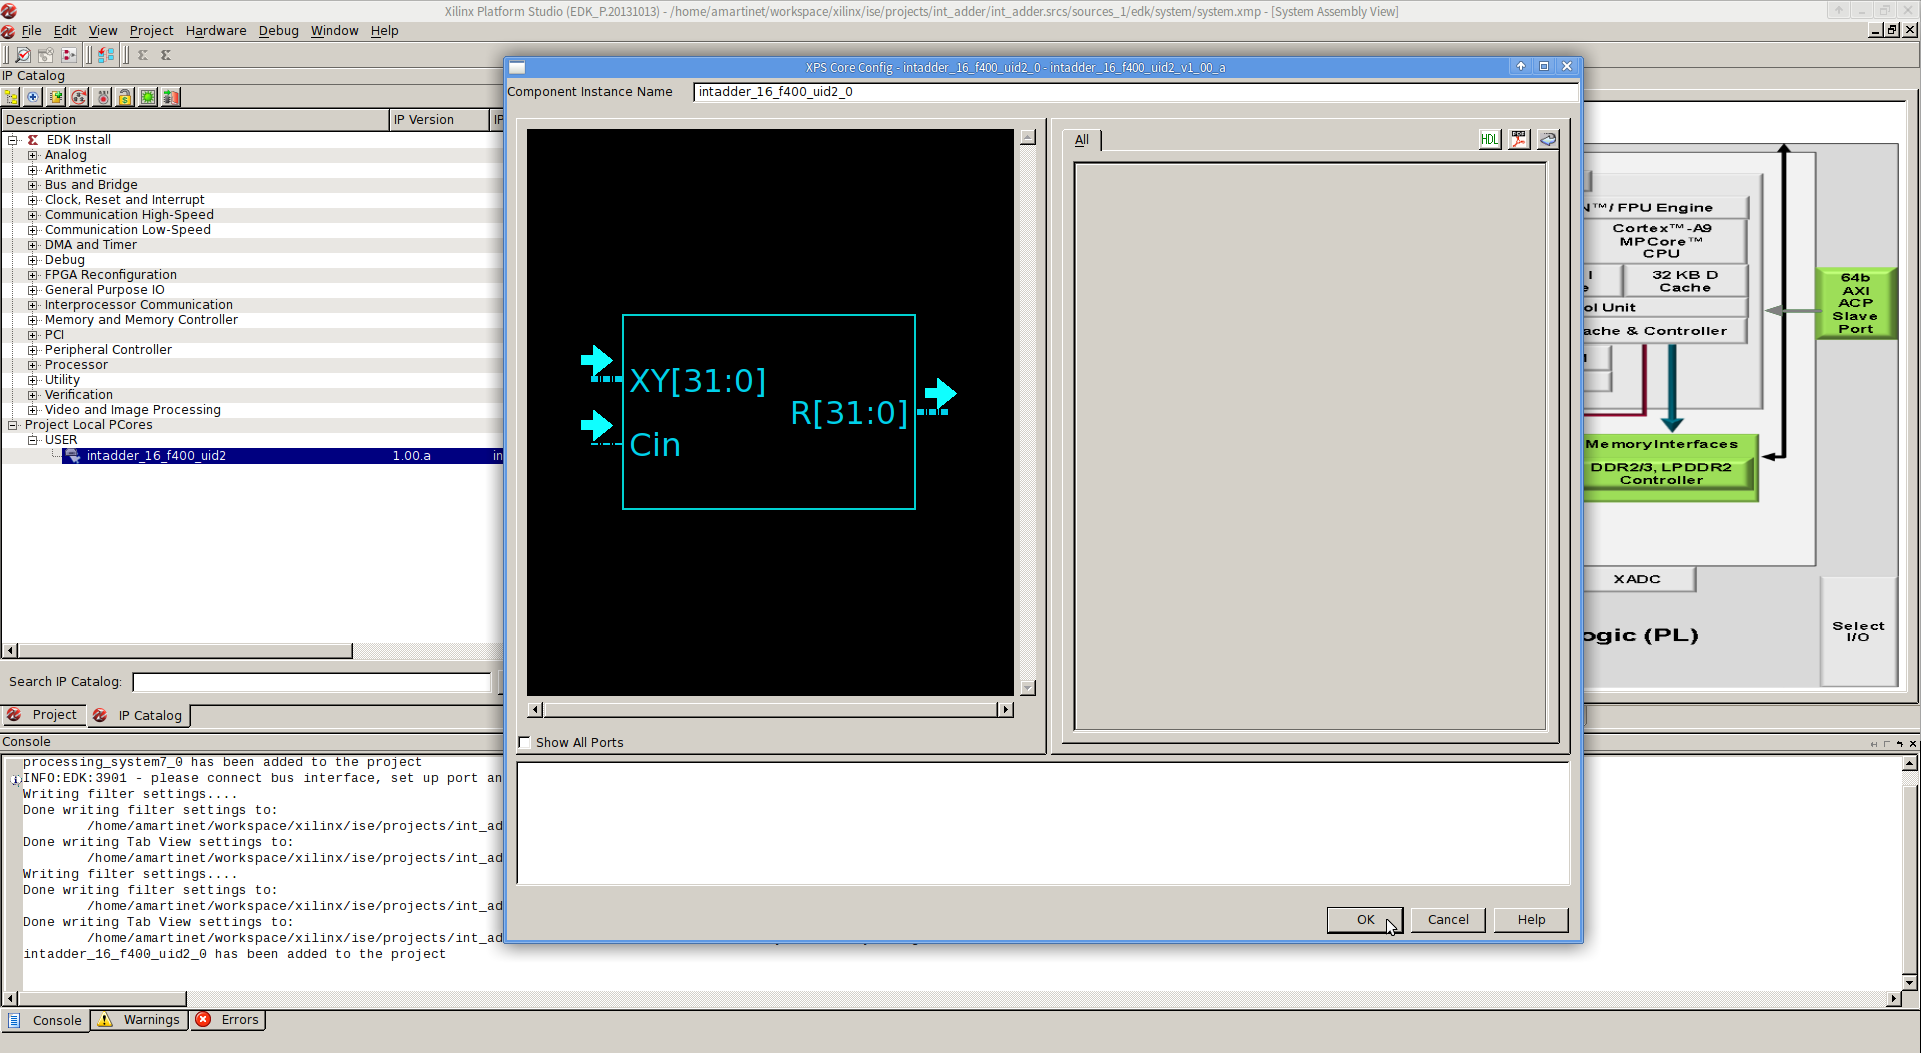
\includegraphics[scale=0.25]{pictures/AddPeripheral3.png}
	\caption{Add custom IP}
	\end{figure}
	\item Now we are going to plug the adder on the GPIO ports.
	\begin{itemize}
		\item click the "Ports" tab.
	\begin{figure}
	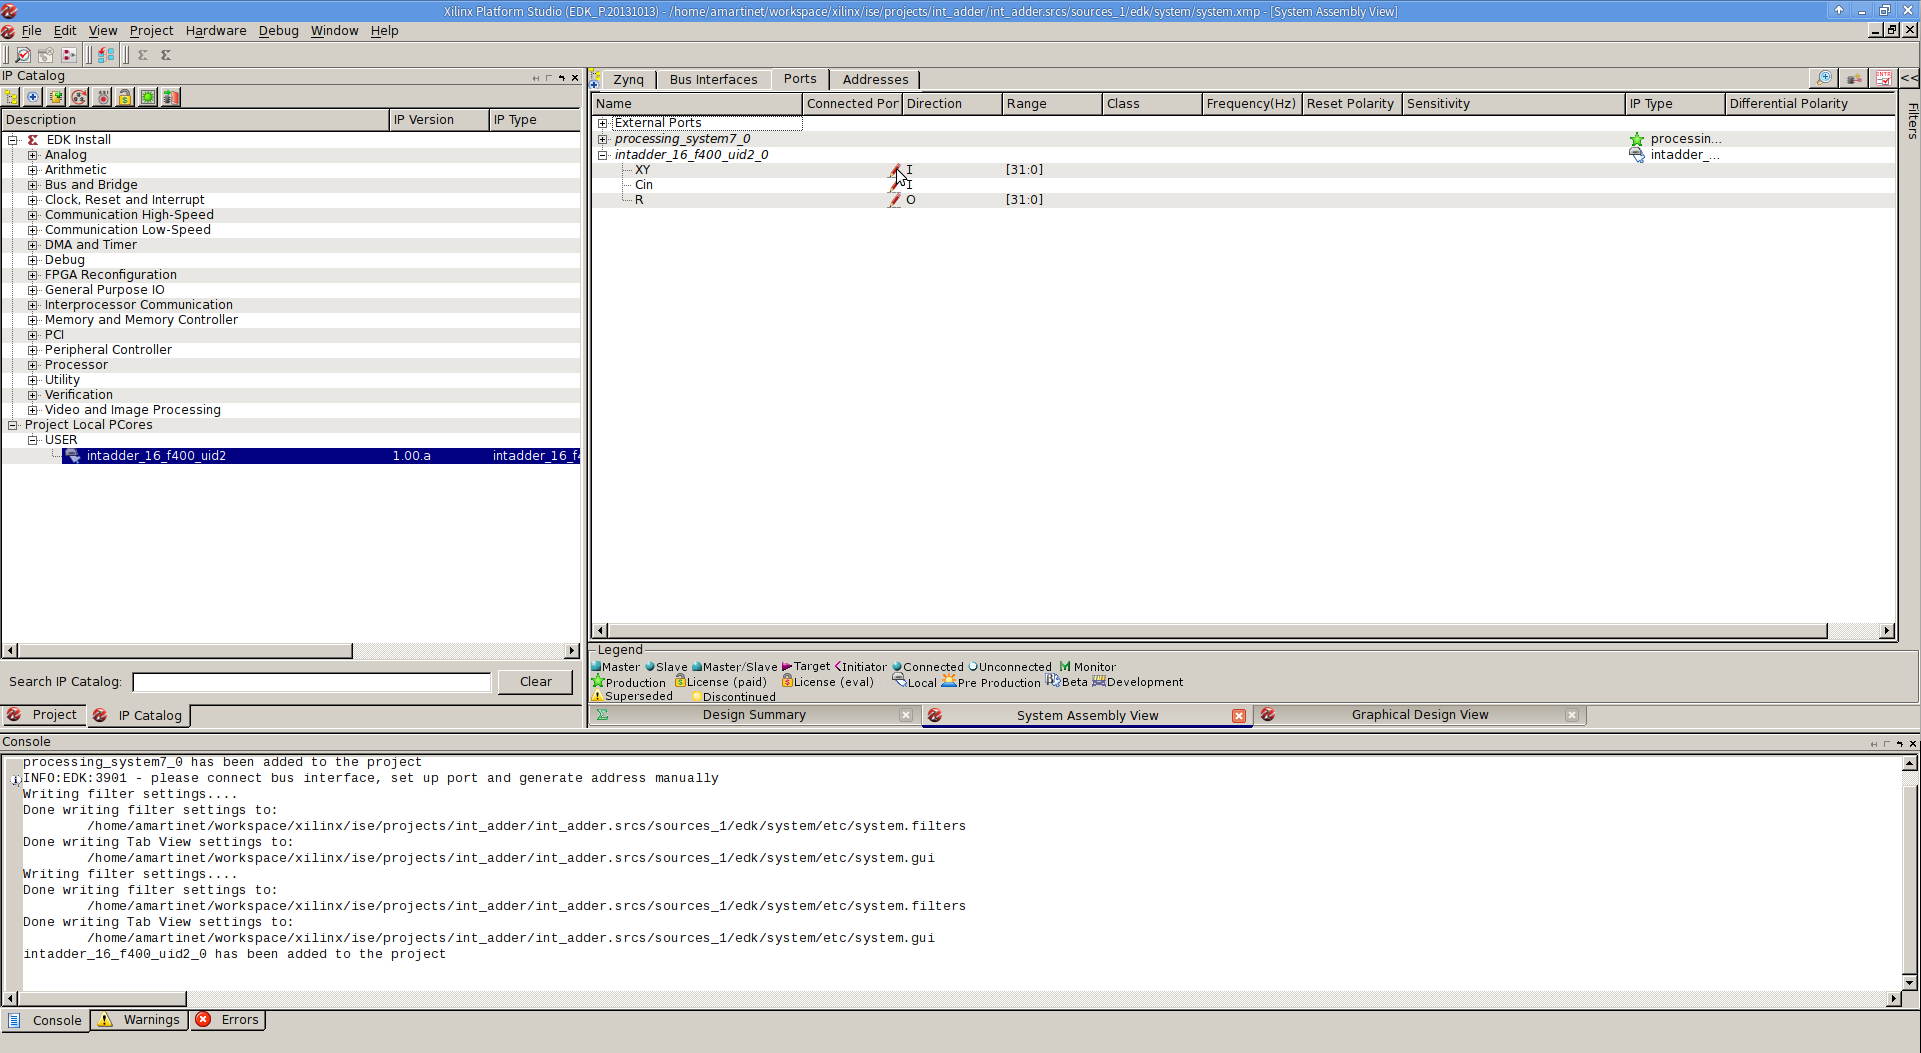
\includegraphics[scale=0.25]{pictures/AddPeripheral4.png}
	\caption{Add custom IP}
	\end{figure}
		\item expand "intadder\_16\_f400\_uid2\_0"
		\item click on the "XY" Connected Port cell (pencil)
		\item select "processing\_system7\_0" on the left drop down menu and
		"[GPIO\_0]::GPIO\_O" on the right one. Click the ok button.
	\begin{figure}
	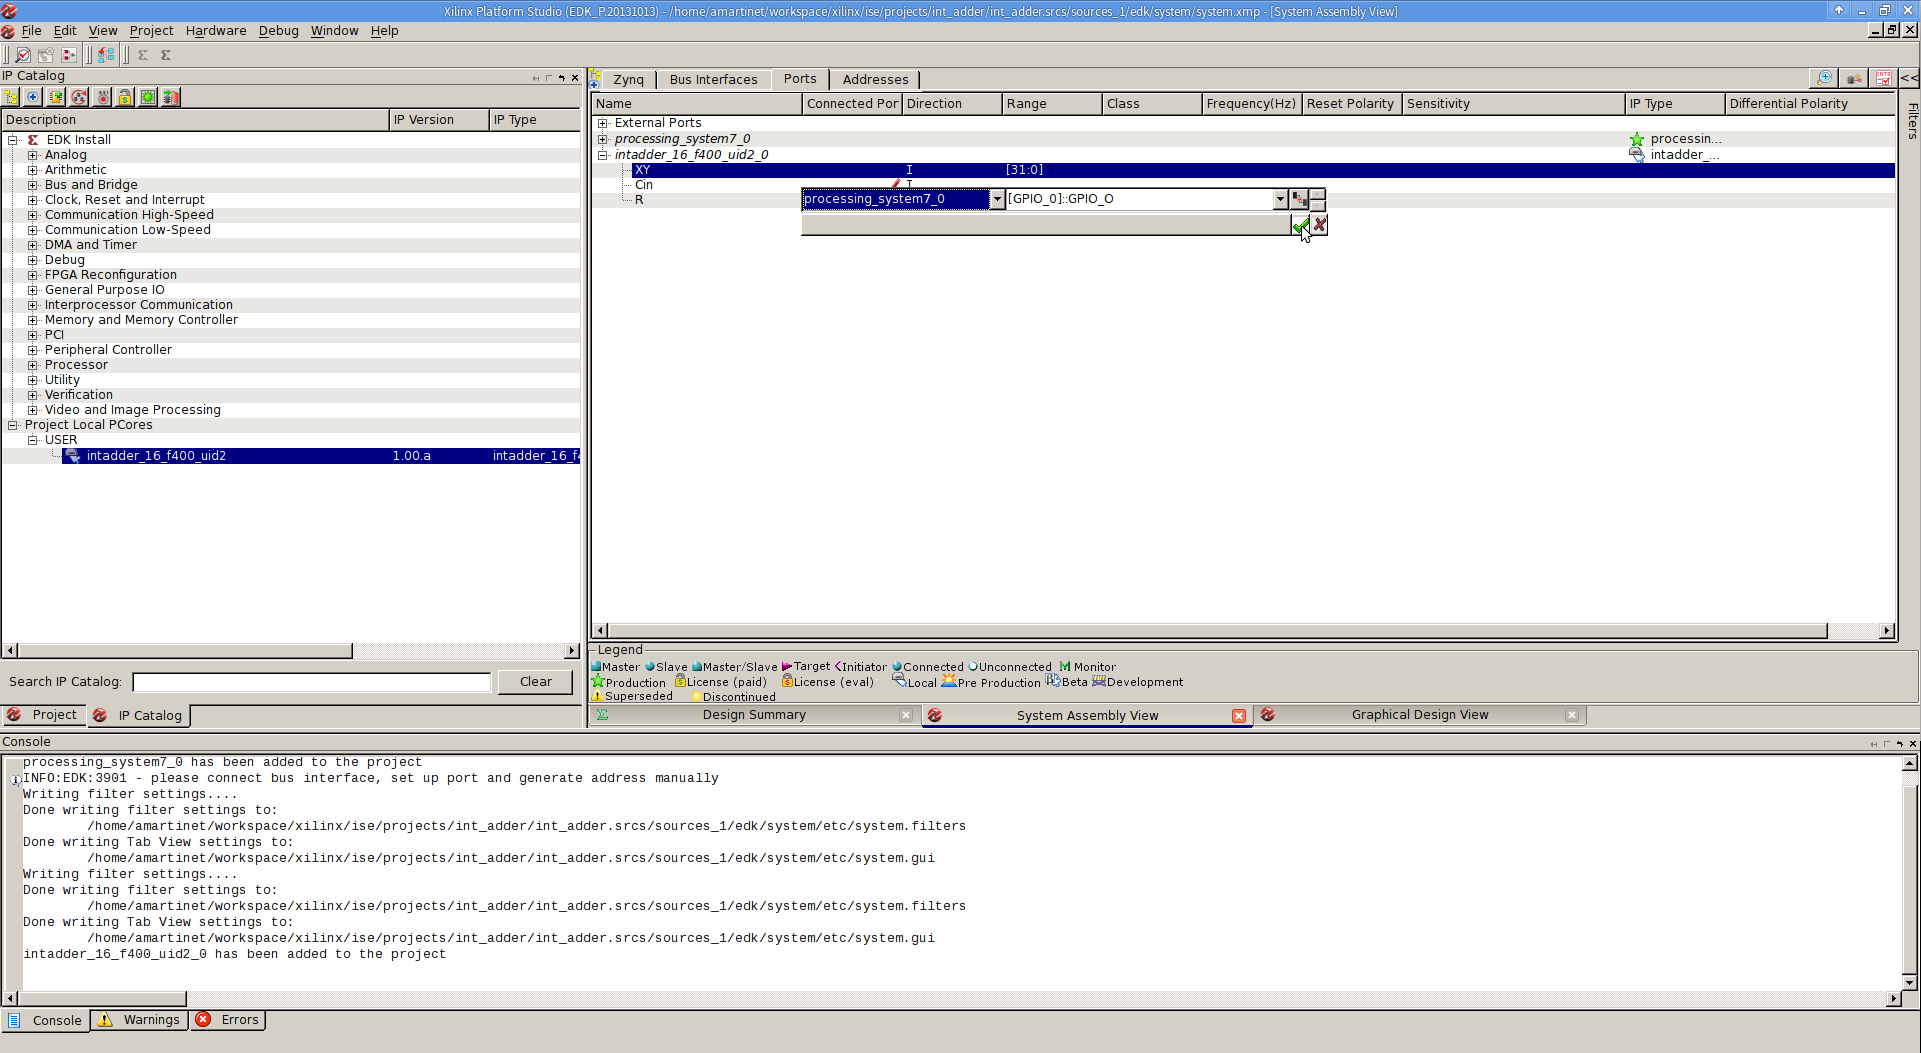
\includegraphics[scale=0.25]{pictures/AddPeripheral5.png}
	\caption{Add custom IP}
	\end{figure}
		\item click on the "R" Connected Port cell
		\item select "processing\_system7\_0" on the left drop down menu and
		"[GPIO\_0]::GPIO\_I" on the right one. Click the ok button.
	\begin{figure}
	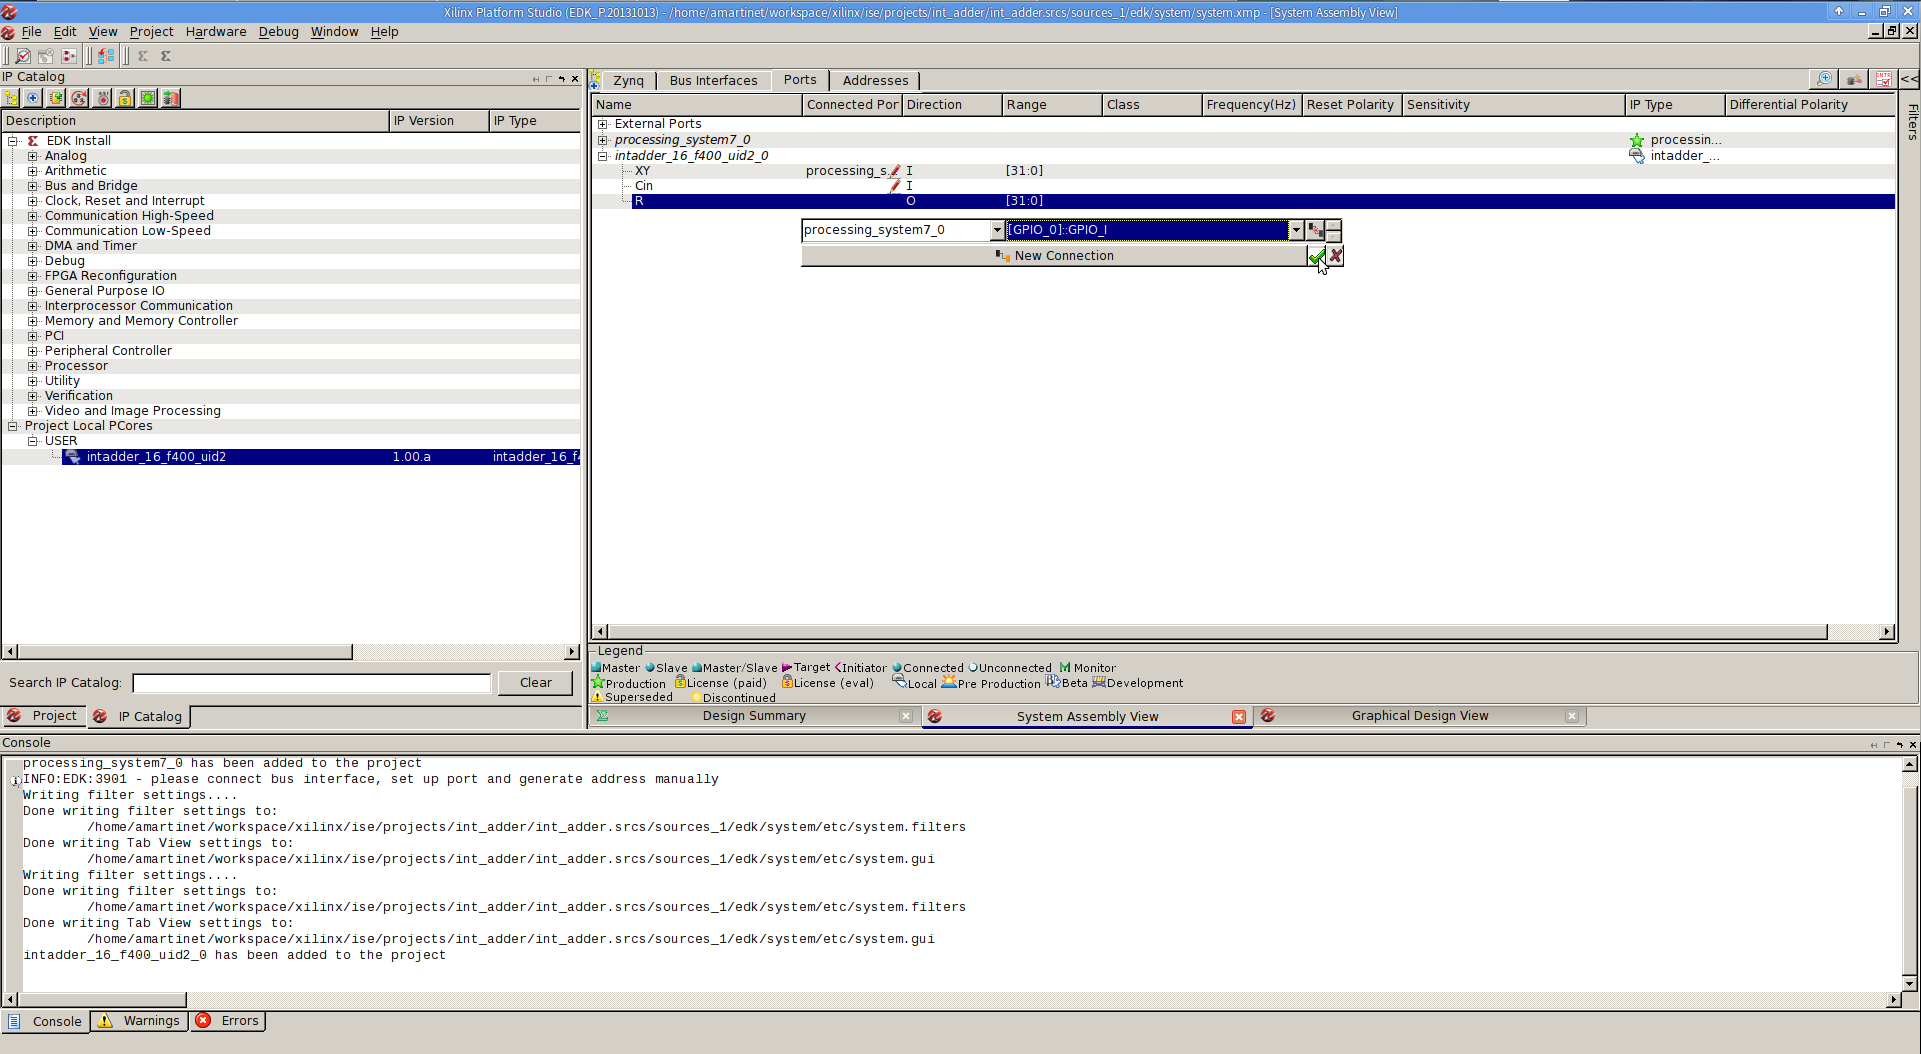
\includegraphics[scale=0.25]{pictures/AddPeripheral6.png}
	\caption{Add custom IP}
	\end{figure}
		\item Cin is not important for this job. (we don't have any remainder to
				add). Leave it be for now.
	\begin{figure}
	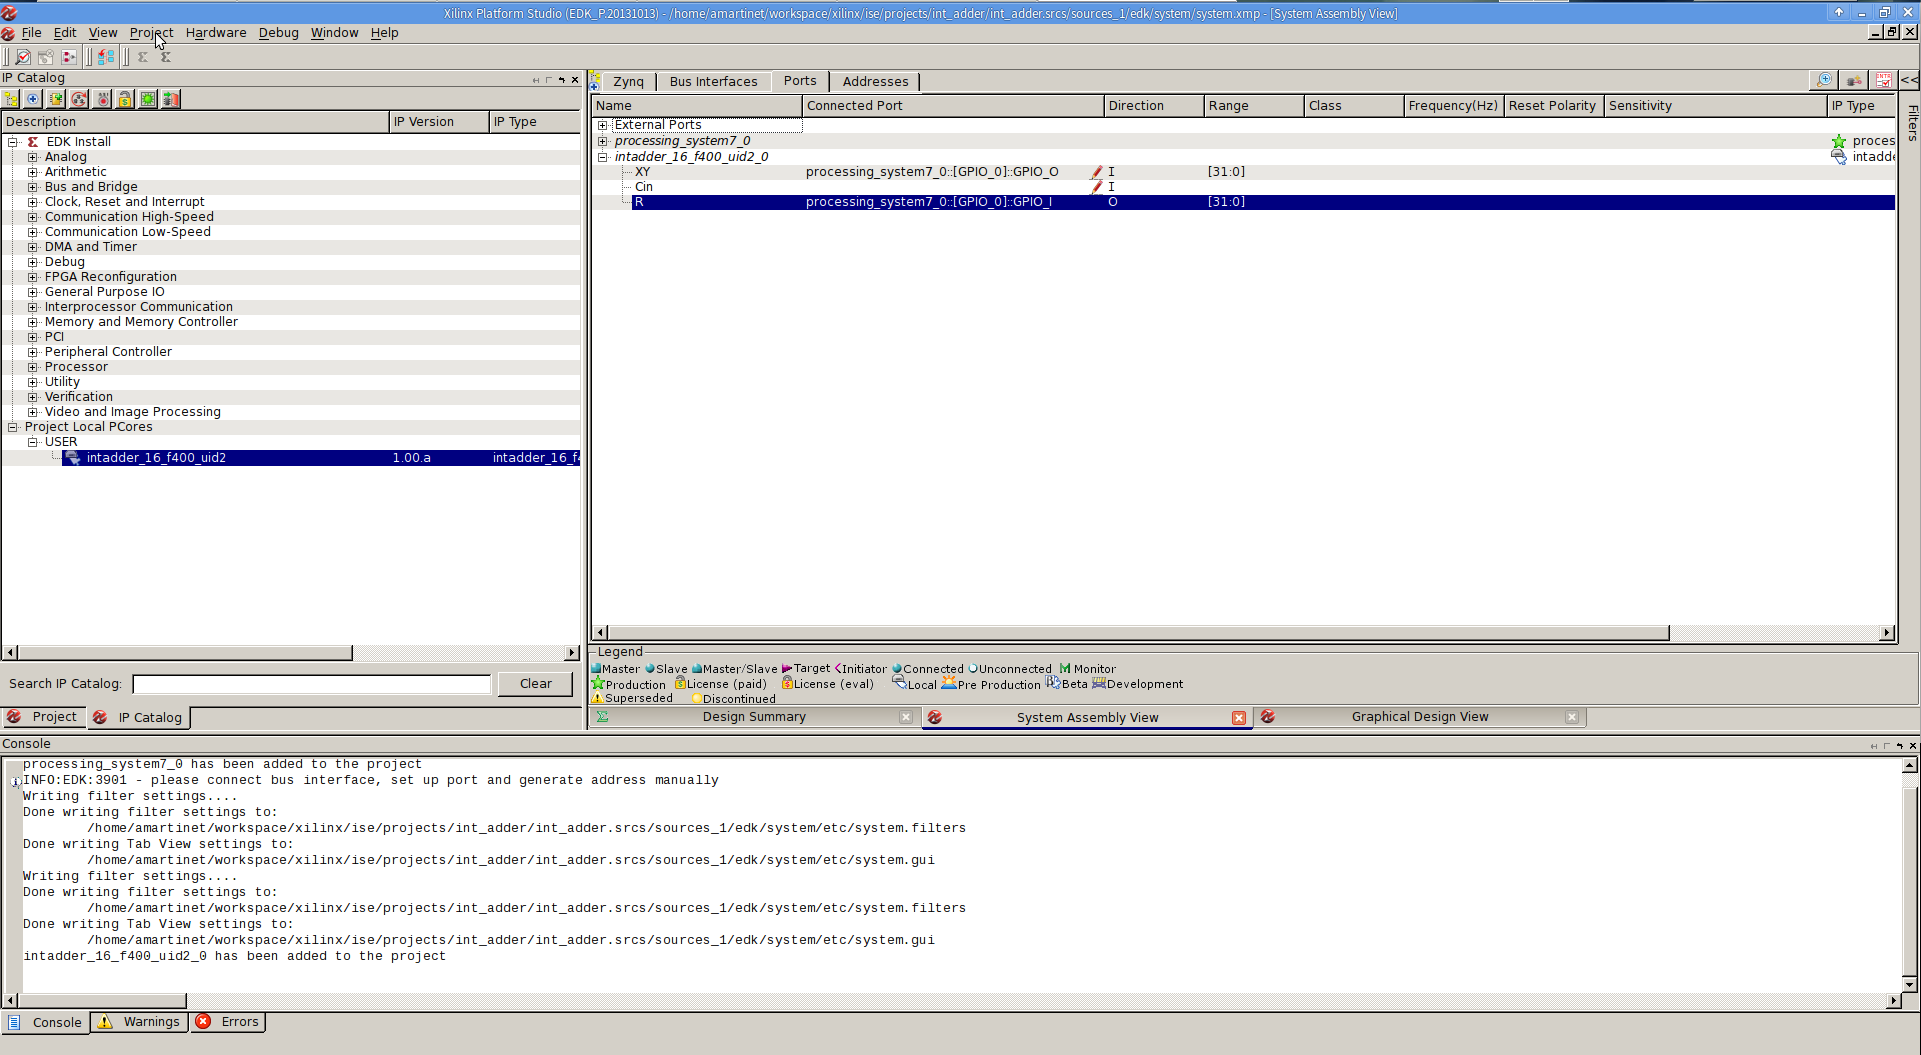
\includegraphics[scale=0.25]{pictures/AddPeripheral7.png}
	\caption{Add custom IP}
	\end{figure}
	\end{itemize}
	\item Run a design rule check and try to fix any error (this should not
			occur).
	\begin{figure}
	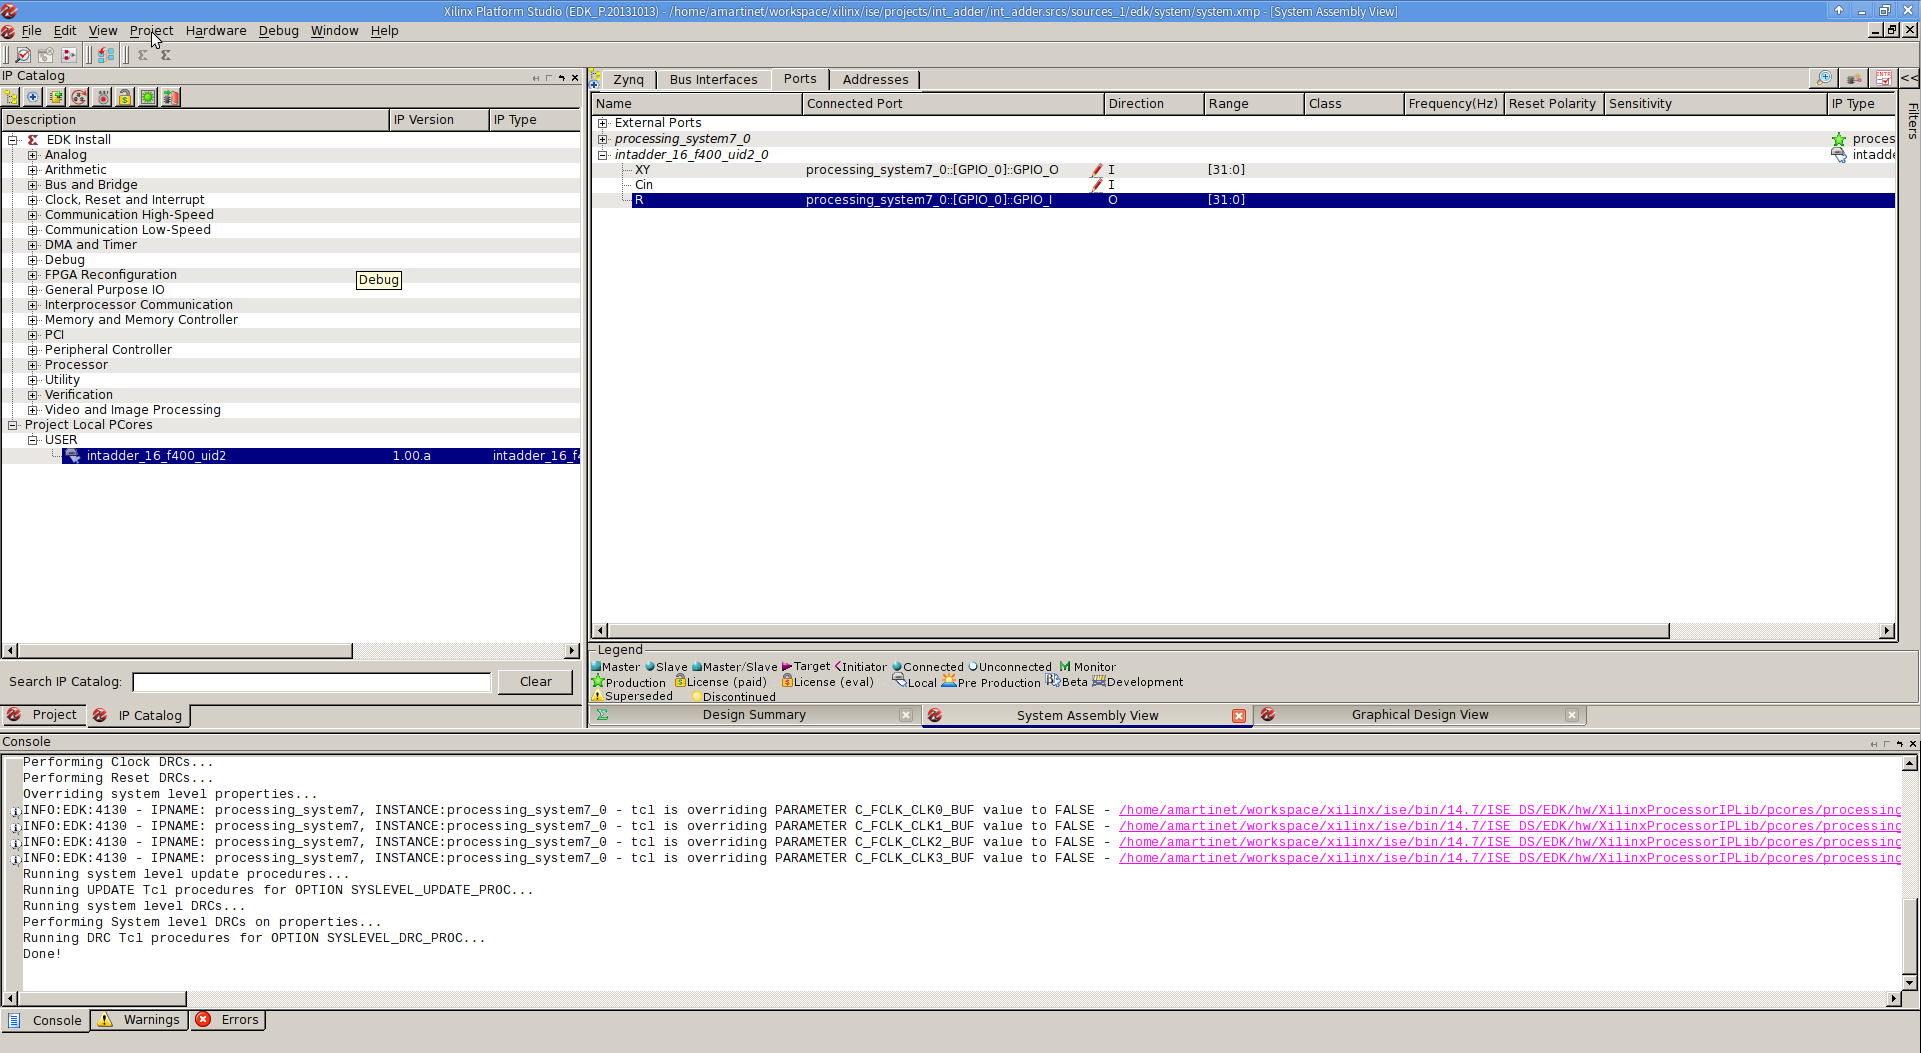
\includegraphics[scale=0.25]{pictures/DesignRuleCheck.png}
	\caption{Design rule check}
	\end{figure}
	\item Close XPS.
	\end{enumerate}
	\section{Generating hardware and drivers}
		\subsection{Generate Hardware}
		Now you know how to design a hardware, let's take a look on the
		compilation chain.
		\begin{enumerate}
		\item First, you need to finish the design sources generation.
		You will see that a new design source popped in the "Sources" panel.
		Right click on "System (system.xmp)", and select "Create Top HDL".
		It will take a short time before the system\_stub.vhd come up.
	\begin{figure}
	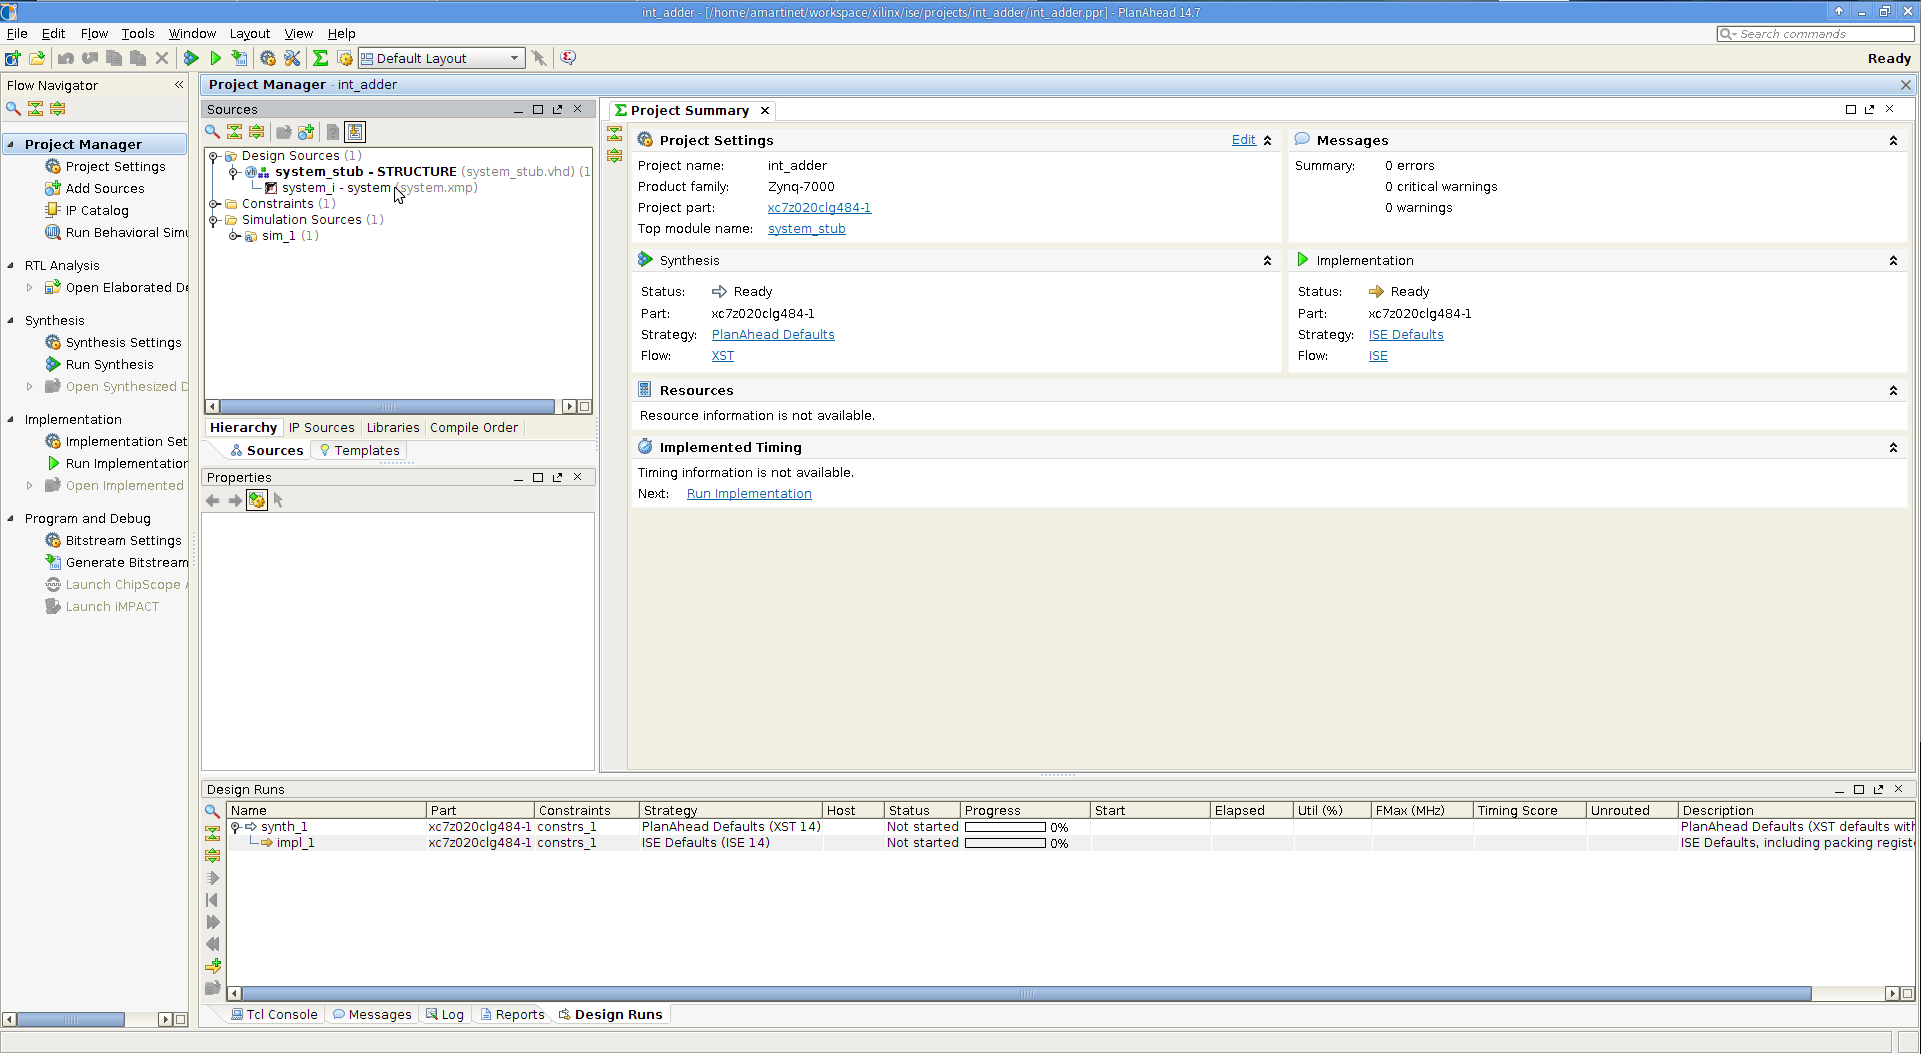
\includegraphics[scale=0.25]{pictures/CreateTopHDL.png}
	\caption{Create top HDL}
	\end{figure}
		\item Then click on "Run Synthesis" in the "Synthesis" menu of the "Flow
		Navigator" panel.
	\begin{figure}
	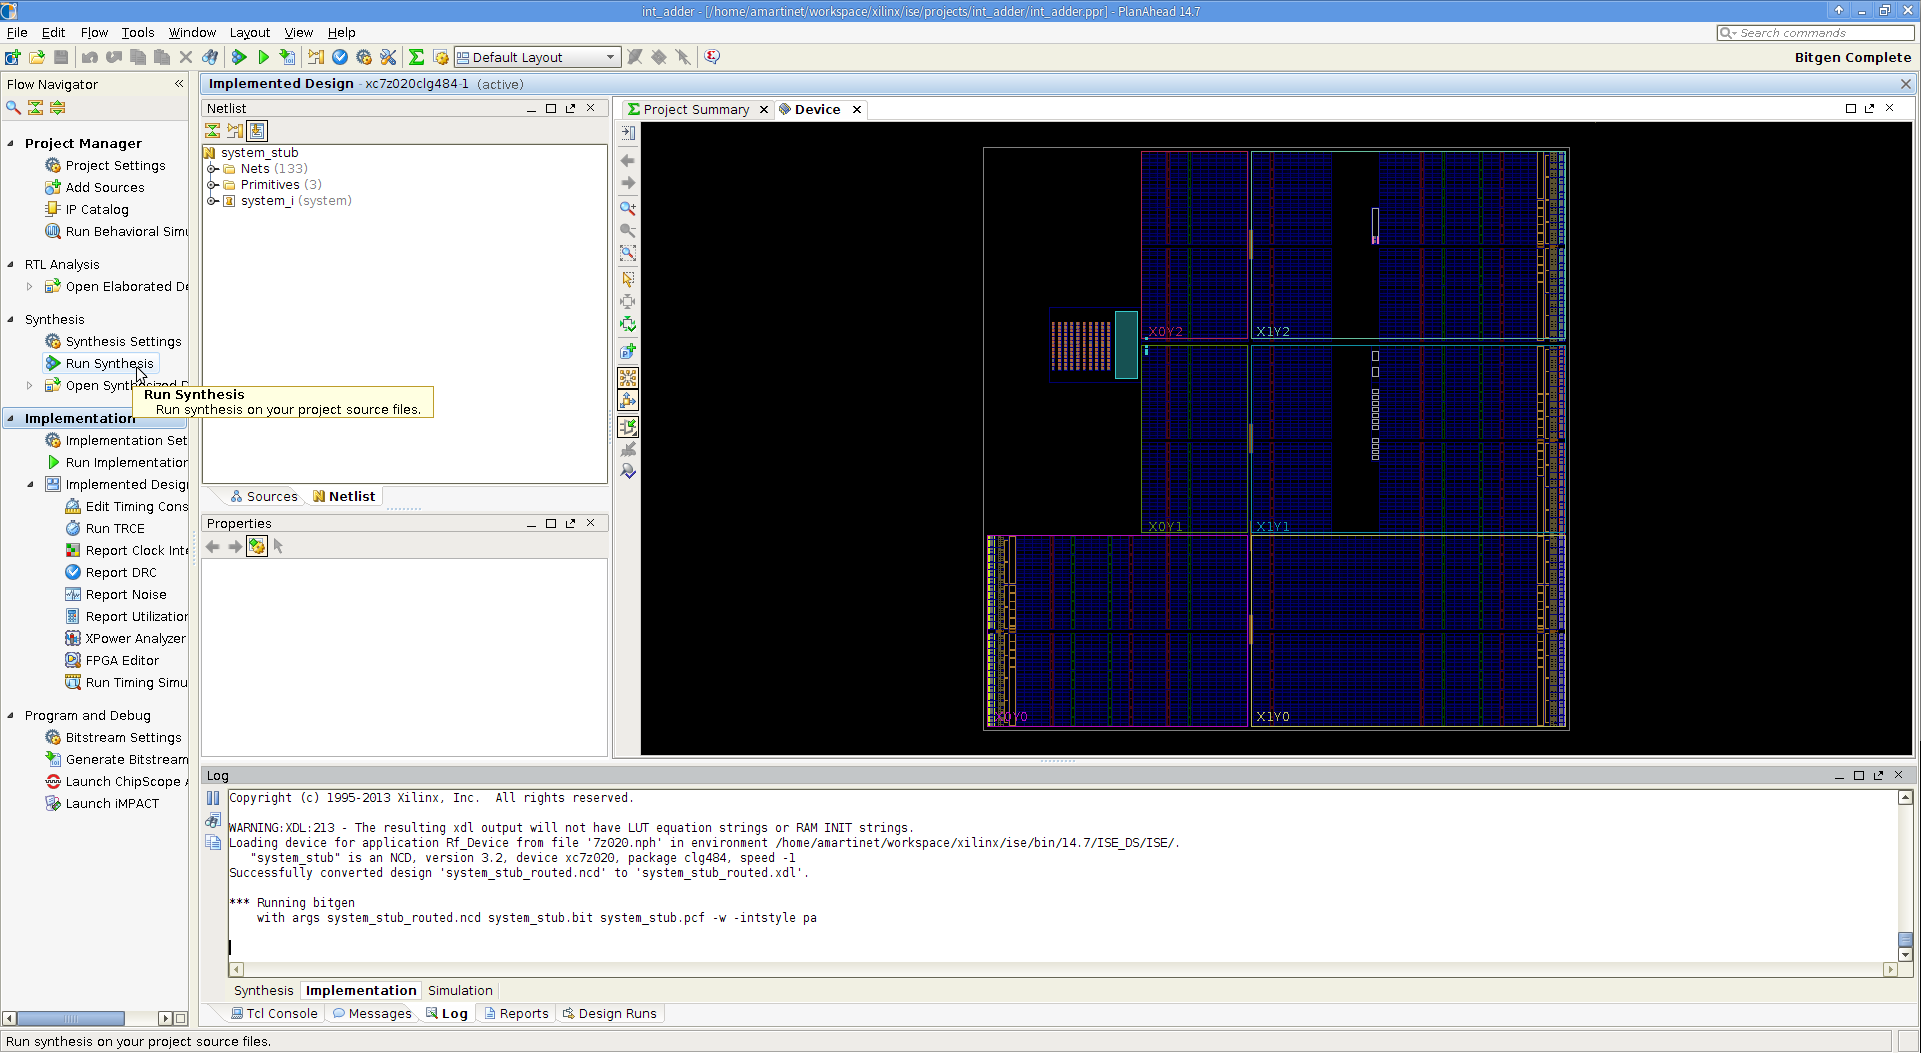
\includegraphics[scale=0.25]{pictures/RunSynthesis.png}
	\caption{Run synthesis}
	\end{figure}
		\item Go make coffee while the synthesis runs.
		\item you are then proposed to perform various actions. Choose the
		default "Run Implementation" and click "OK".
	\begin{figure}
	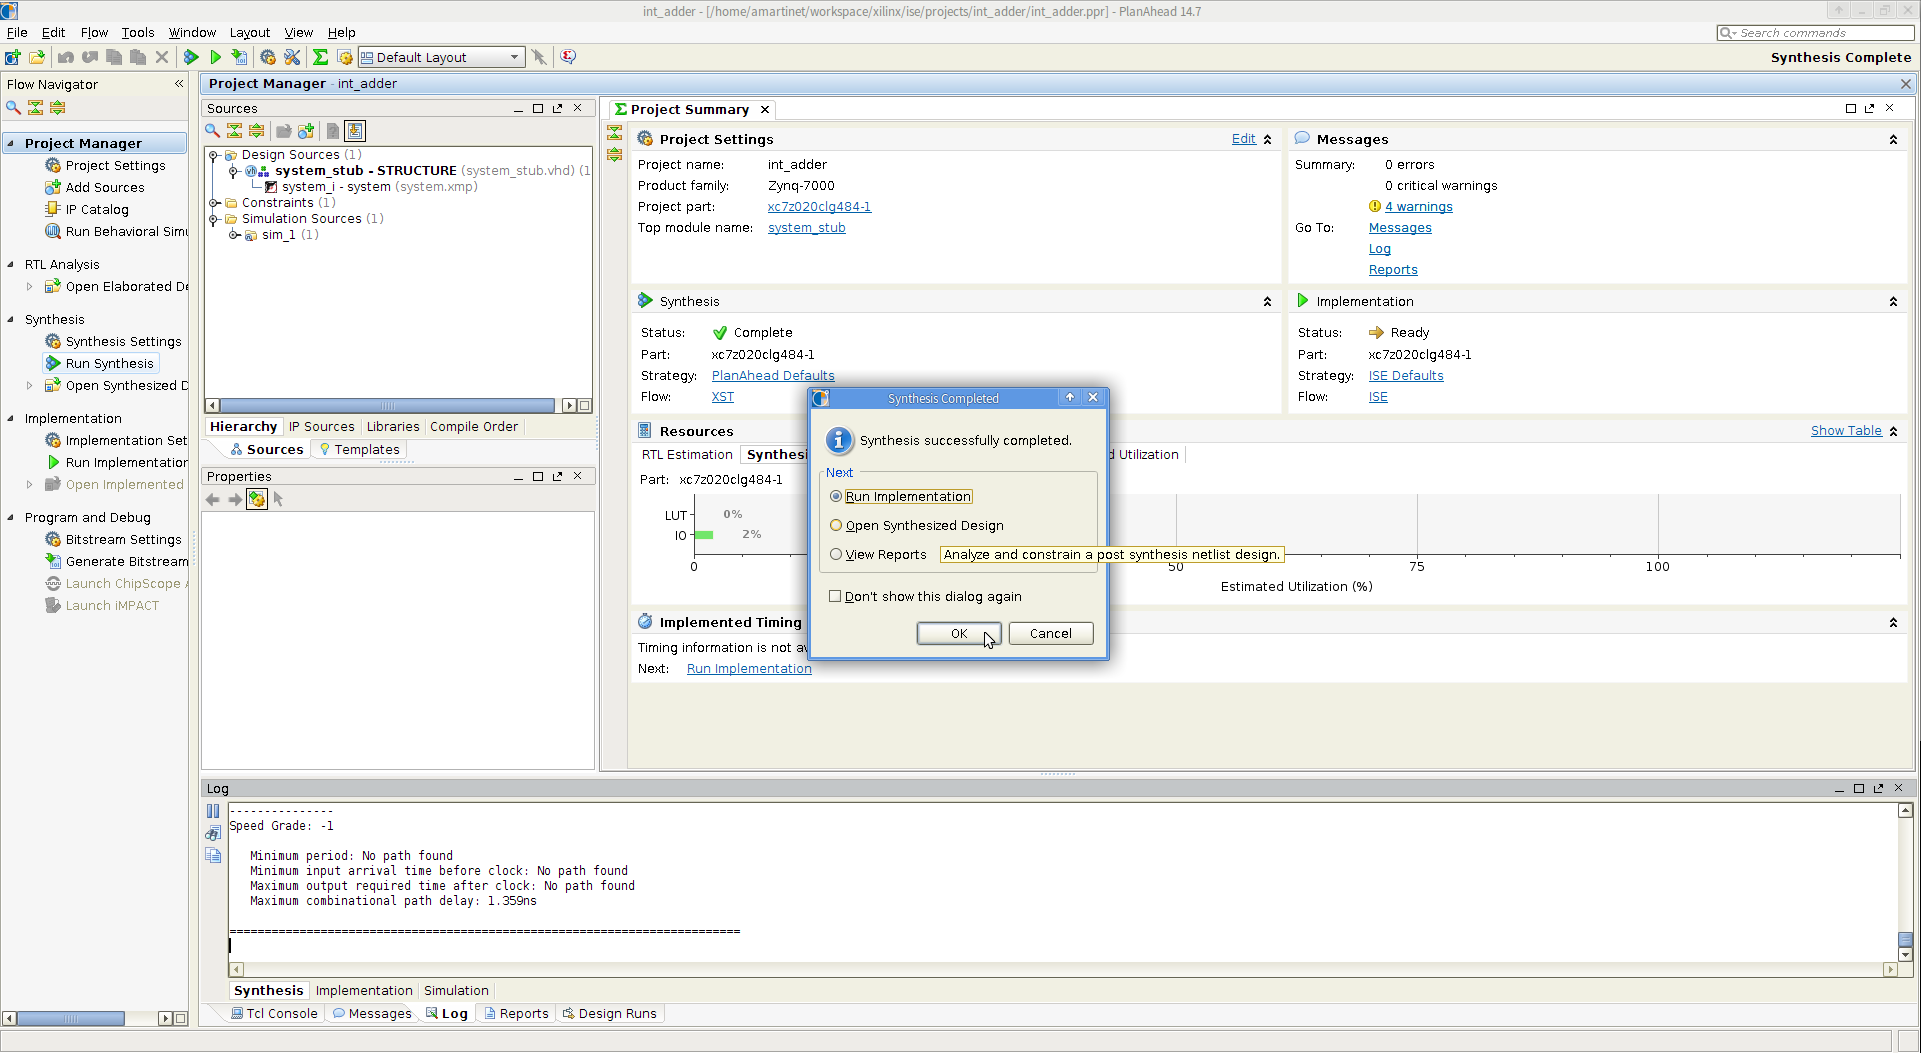
\includegraphics[scale=0.25]{pictures/SynthesisComplete.png}
	\caption{Run implementation}
	\end{figure}
		\item Go drink your coffee.
		\item You will then get (usually 3) critical warnings about IBUF pins.
		Don't care of them and click ok to the boxes.
	\begin{figure}
	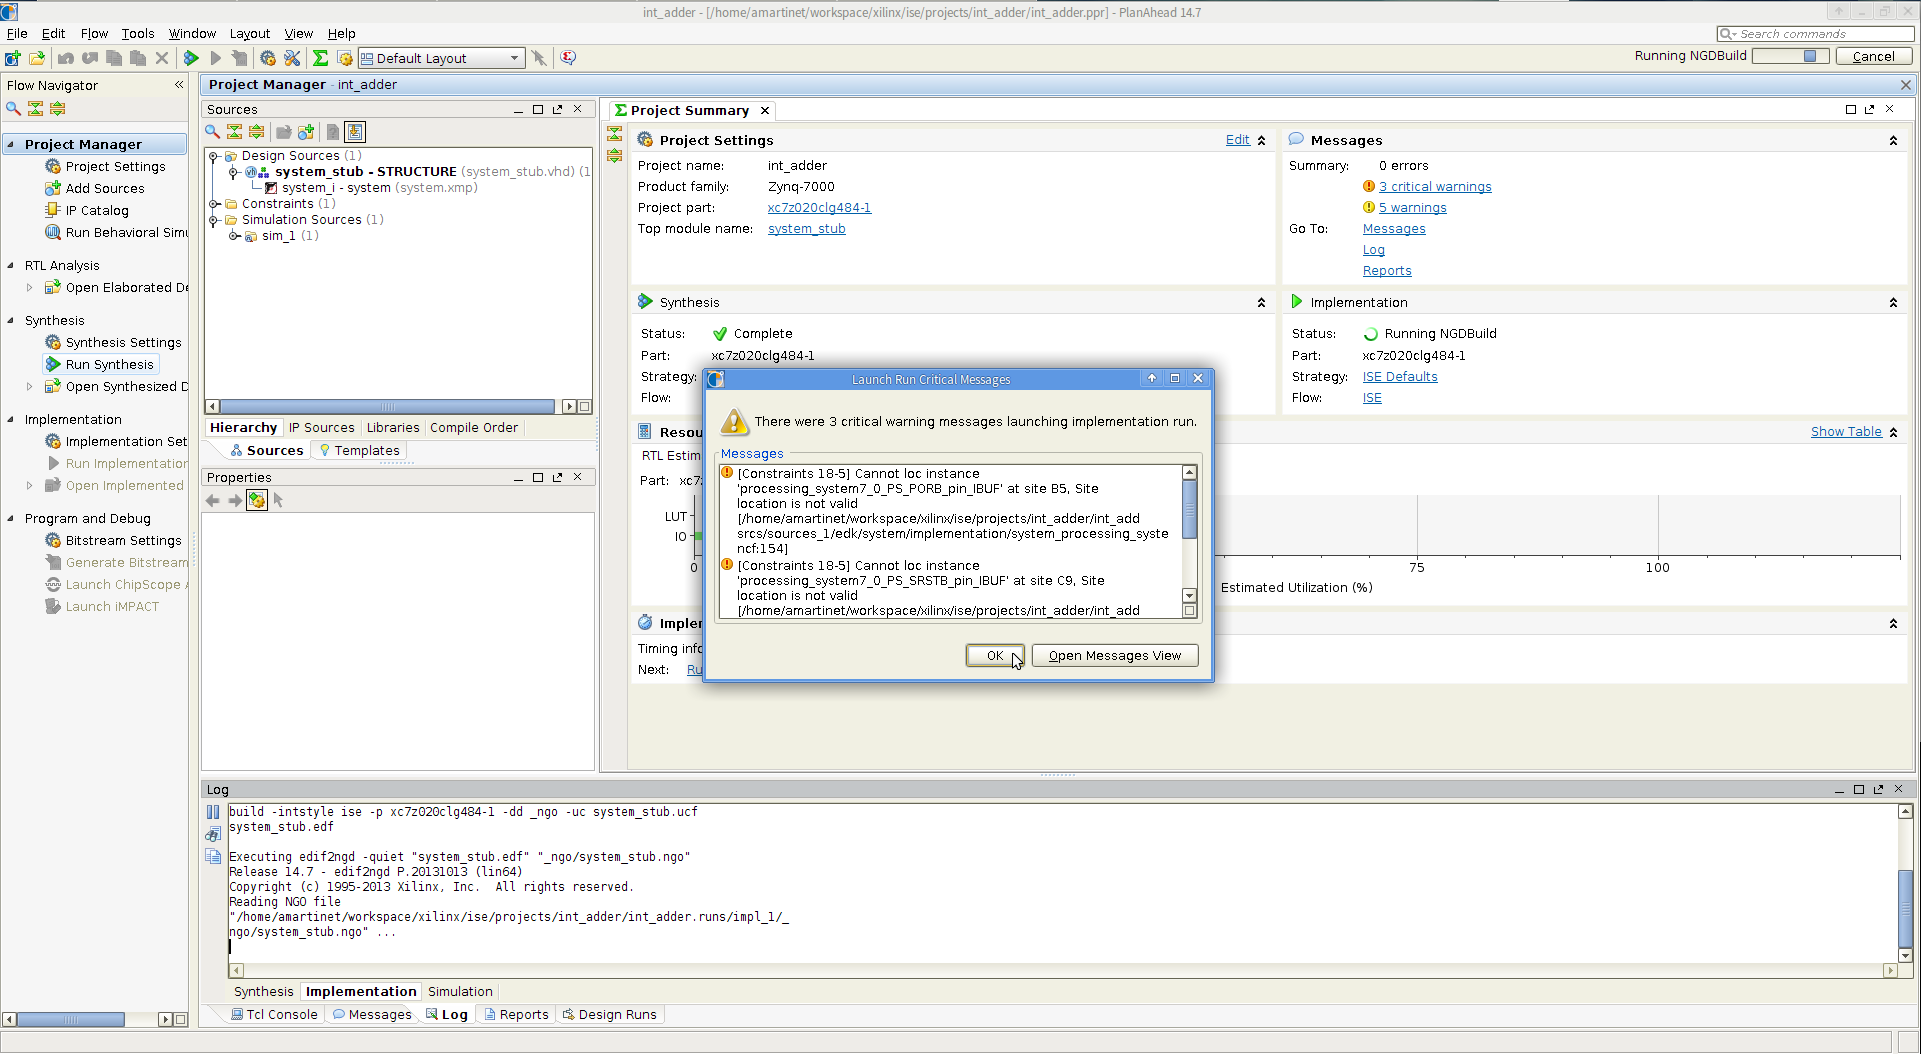
\includegraphics[scale=0.25]{pictures/CriticalWarnings.png}
	\caption{Critical warnings}
	\end{figure}
		\item Then you will be asked again to perform various actions. Here I
		will choose "Open Implemented Design". You can also choose "Generate
		Bitstream", but remember you'll have to open the implemented design to
		be able to perform the later "Export Hardware" operation. This will be
		done using the "Open Implemented Design" option in the Flow Navigator.
		So for now, choose the default "Open Implemented Design". Wait for it to be read and
		displayed. Don't take care of the warnings, actually, you have already
		seen those ones at the synthesis step.
	\begin{figure}
	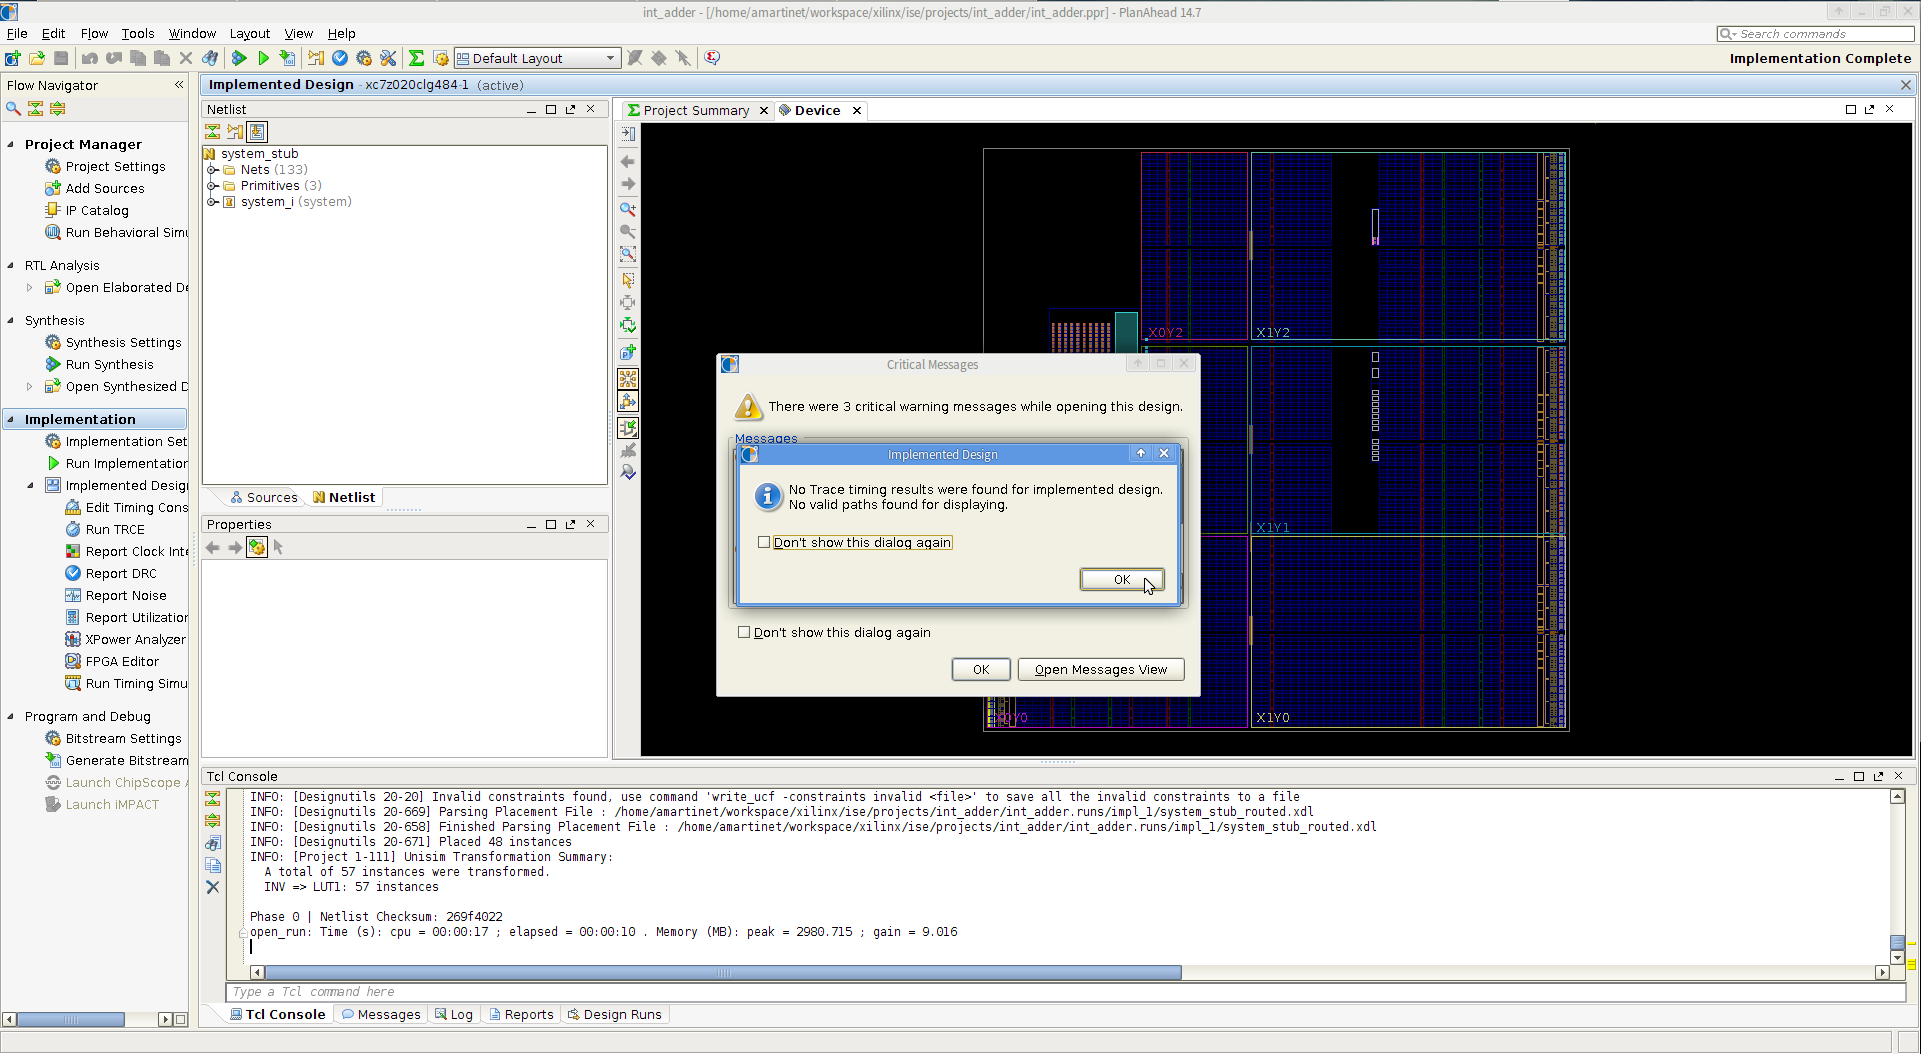
\includegraphics[scale=0.25]{pictures/CritsAgain.png}
	\caption{Critical warnings on implementation openning}
	\end{figure}
		\item Then click "Generate Bitstream" in the Flow Navigator. For further
		runs, I have to tell you that clicking it direct after the top HDL
		generation will result in doing all the precedent actions but the implementing design
		opening.
	\begin{figure}
	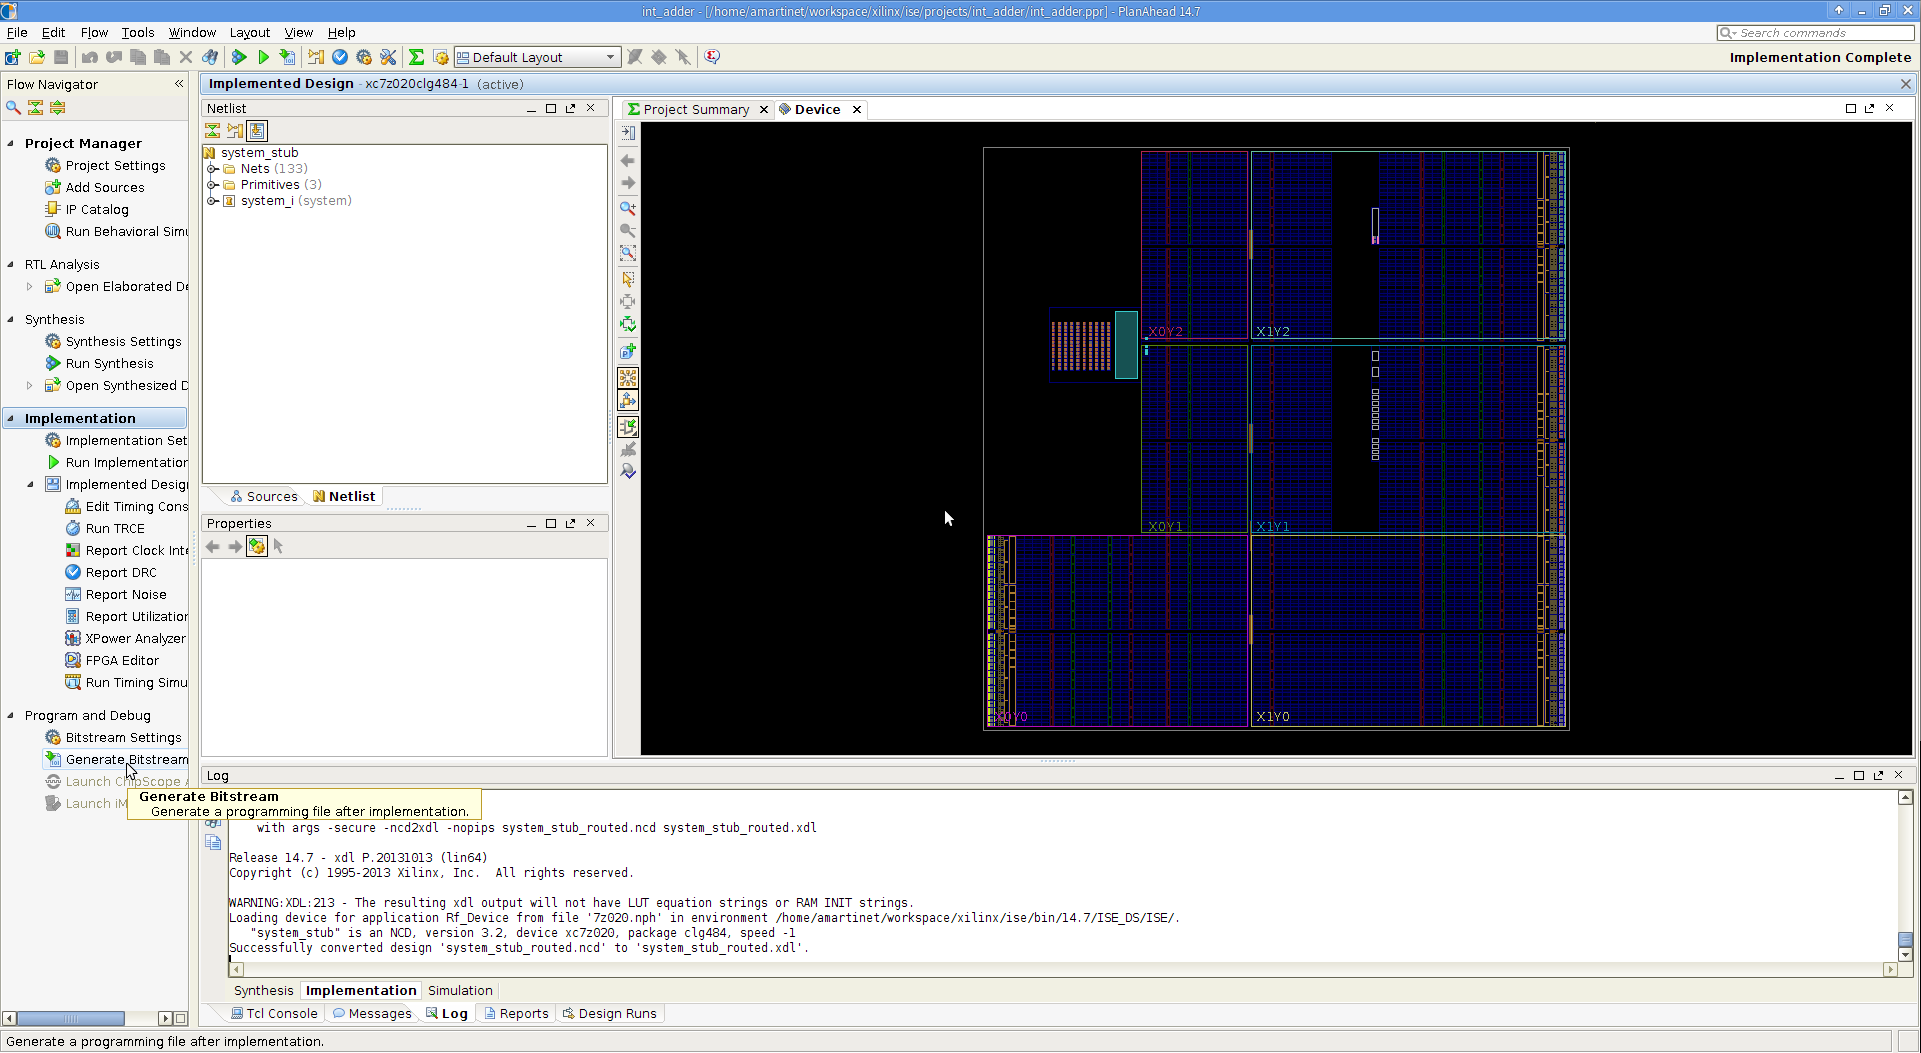
\includegraphics[scale=0.25]{pictures/GenerateBitstream.png}
	\caption{Generate bitstream}
	\end{figure}
		\item Take a little rest waiting Bitgen script to complete.
		\item Then click the menu "File" -> "Export" -> "Export	Hardware for SDK".
		\item Check the three boxes ("Include Bitstream", "Export Hardware" and
				"Launch SDK"). Click "OK". Wait for SDK to launch.
	\begin{figure}
	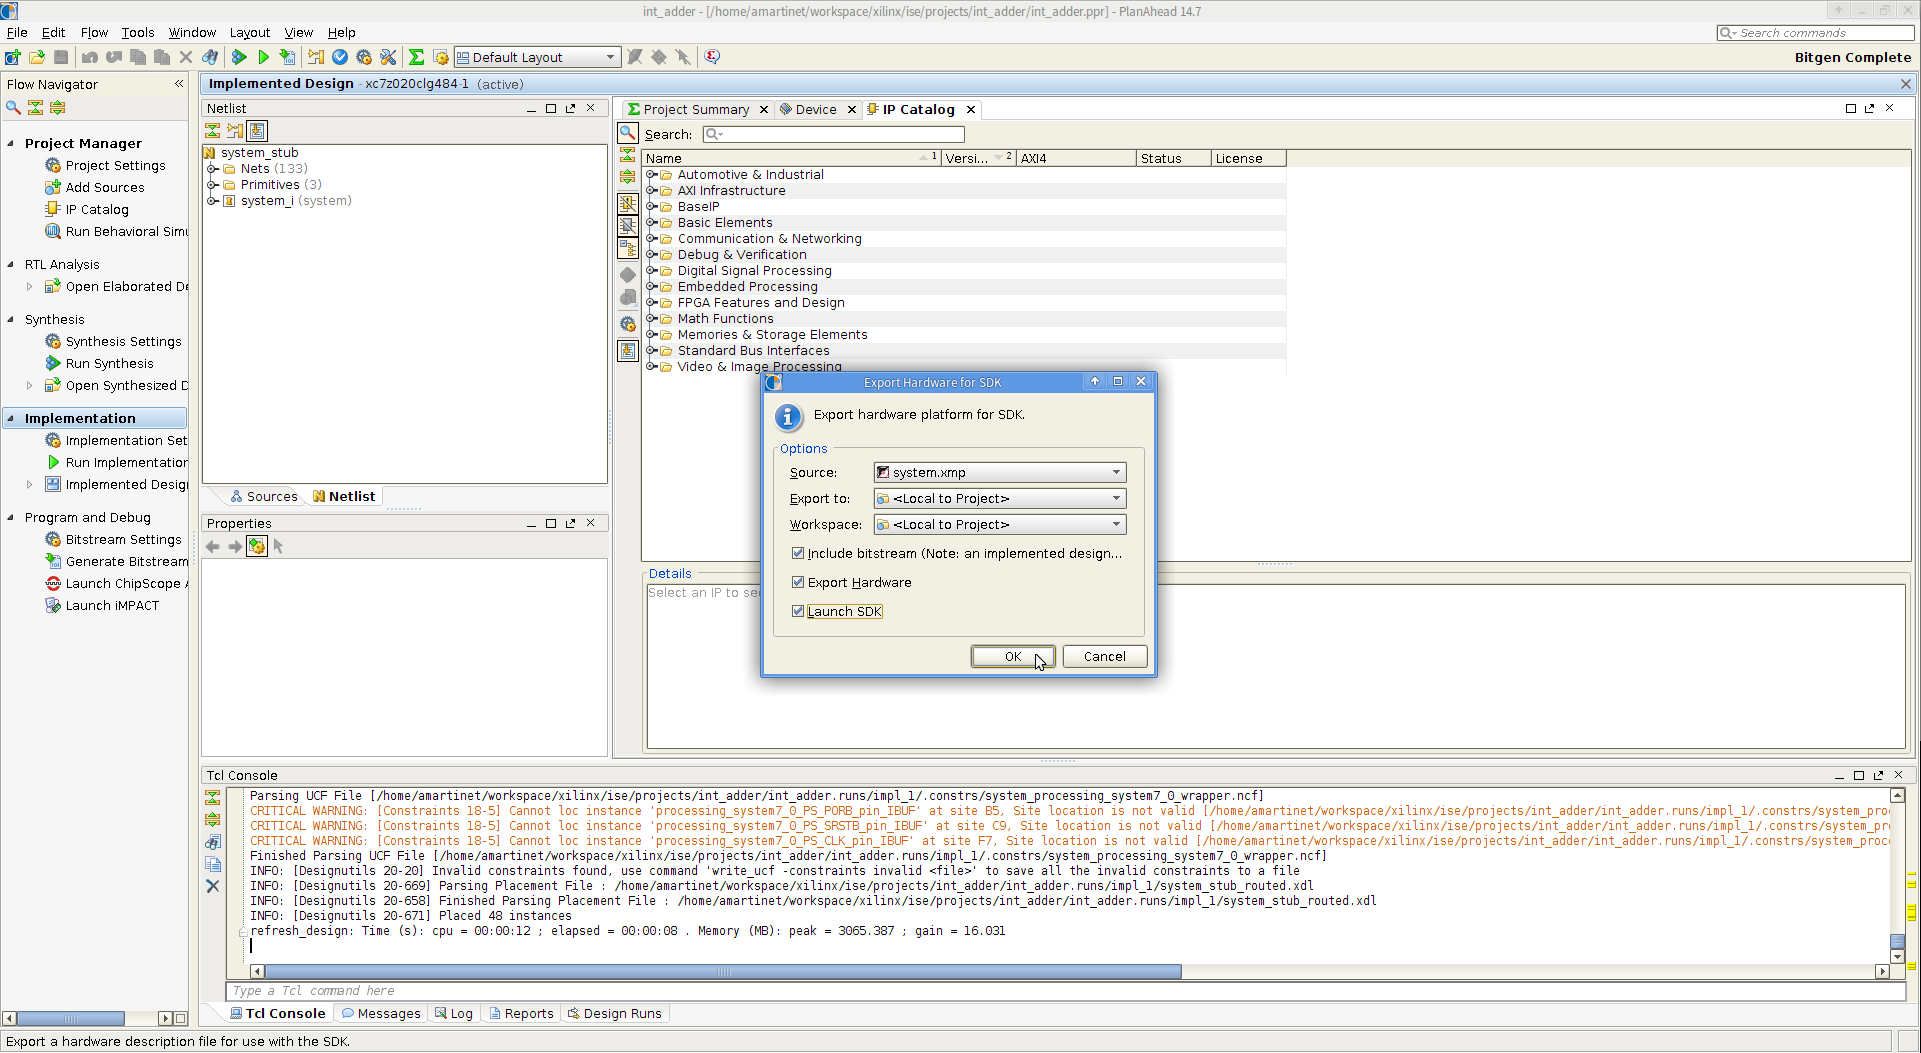
\includegraphics[scale=0.25]{pictures/ExportHardware.png}
	\caption{Export hardware}
	\end{figure}
		\end{enumerate}

	\section{Peripheral full test}
		Now the peripheral is configured and "drived", 
		Let's take a look about it's good functionnality.
		First, you will create a new project and create code for getting
		information from your new peripheral.
		\subsection{Creating a new C project}
		You first need to create a new project.
		For this purpose, get through the following steps:\\
			\begin {enumerate}
			\item Go to "File" -> "New" -> "Project"
	\begin{figure}
	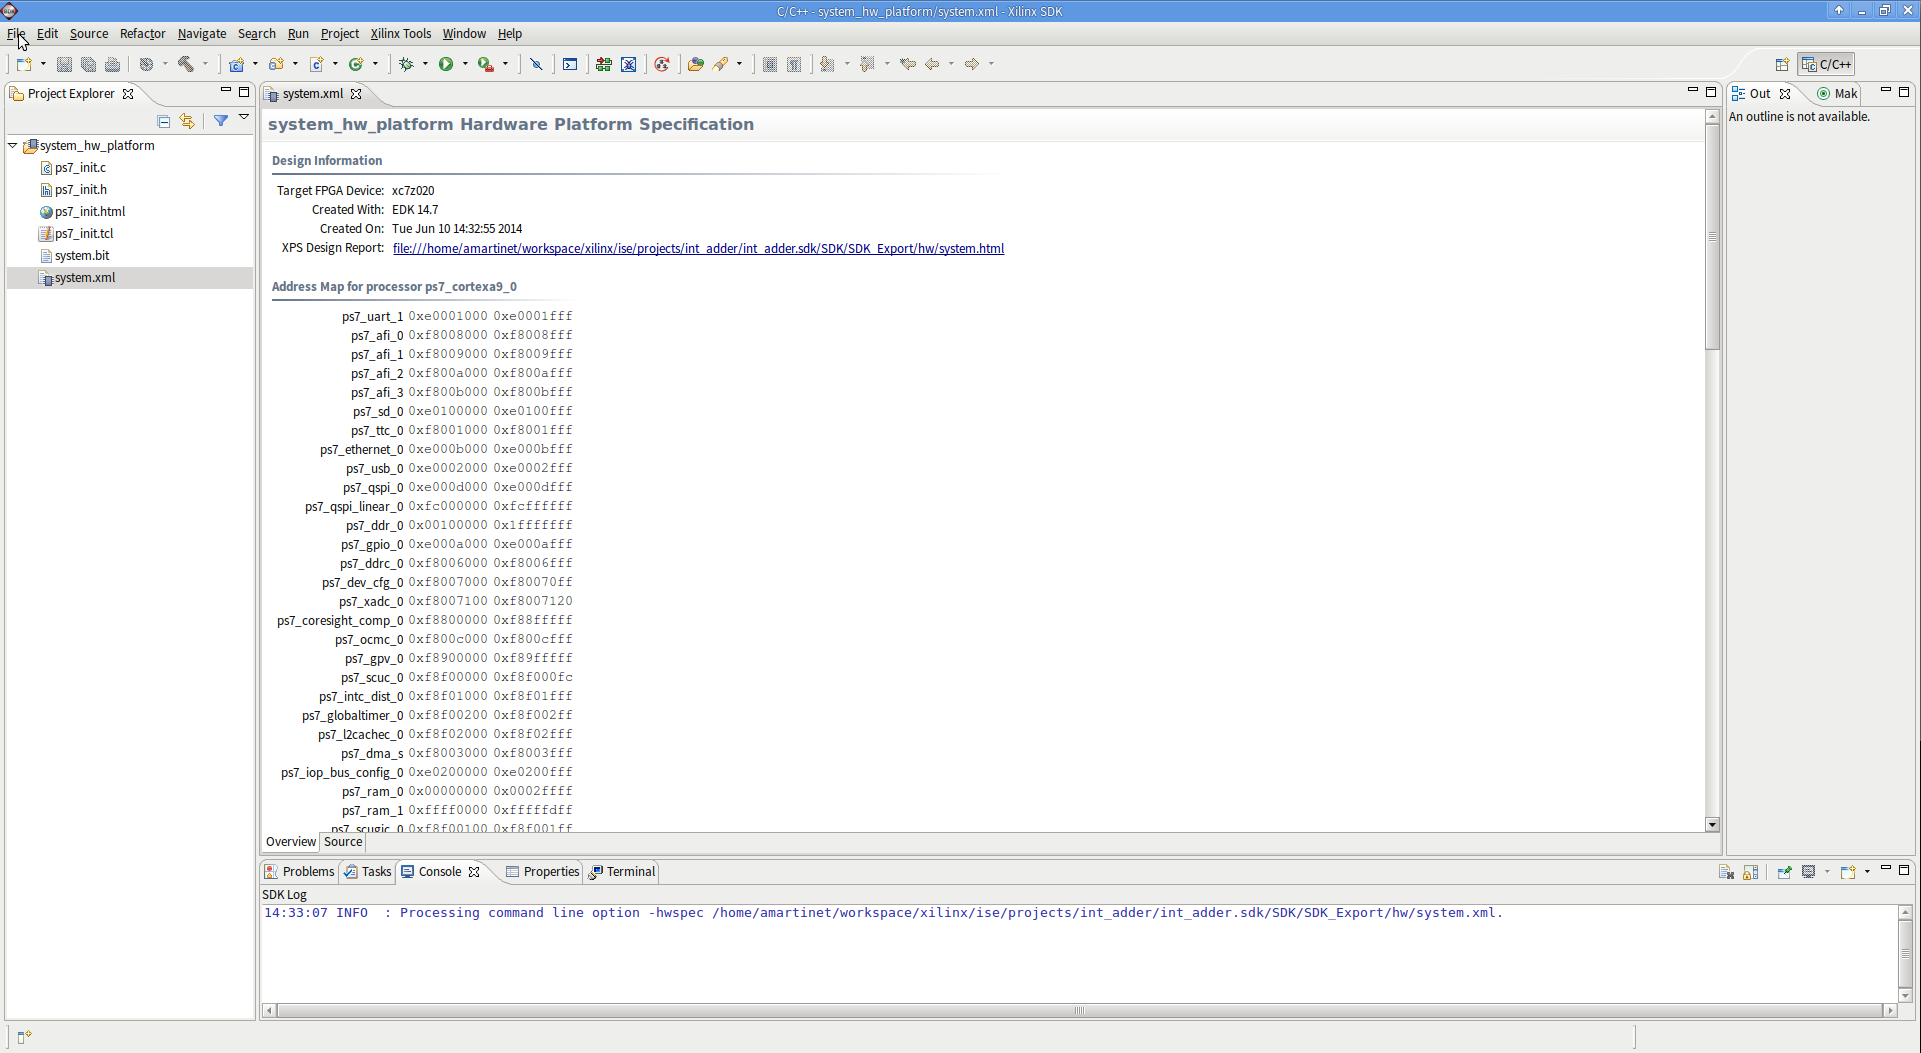
\includegraphics[scale=0.25]{pictures/XSDKMain.png}
	\caption{Xilinx SDK start window}
	\end{figure}
			\item Expand "Xilinx" and select "Application Project". Click
			"Next".
	\begin{figure}
	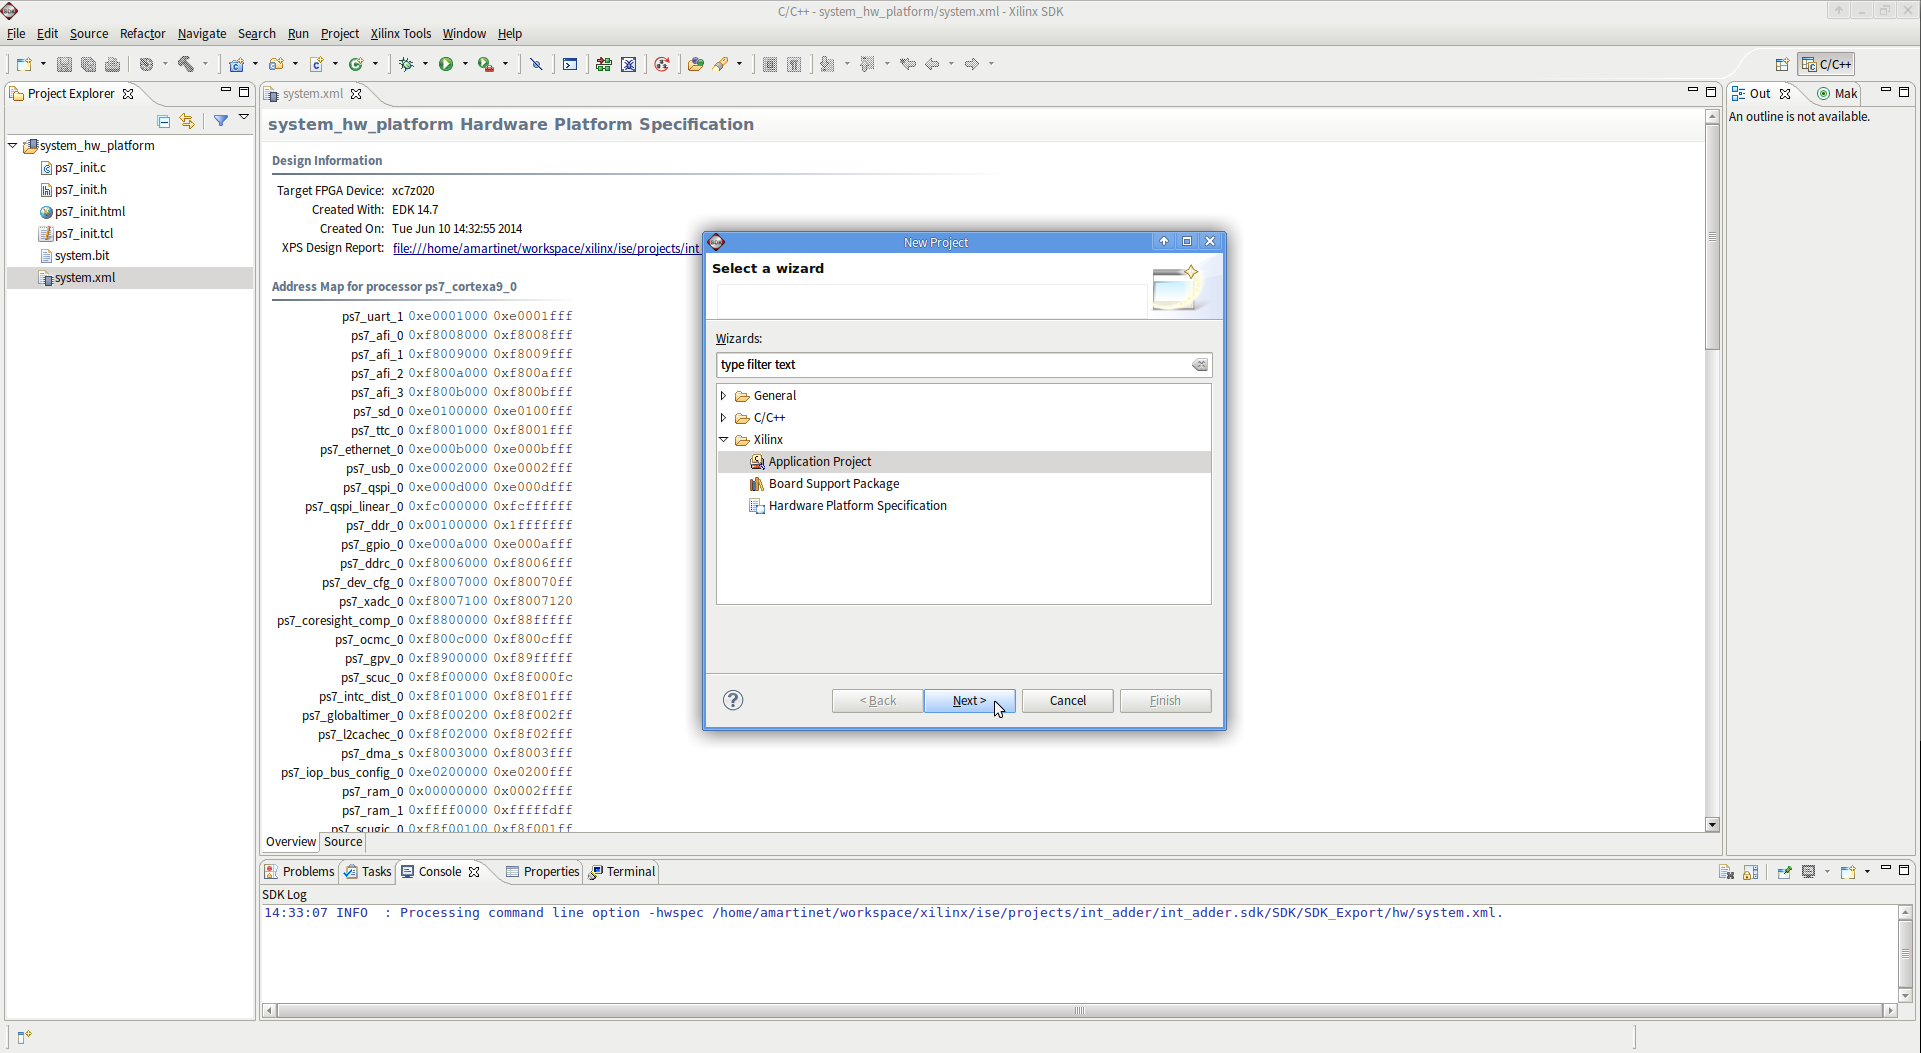
\includegraphics[scale=0.25]{pictures/XSDKNewProject1.png}
	\caption{Export hardware}
	\end{figure}
			\item Give a name to your project. For example, I use int\_add\_16.
			Leave everything as it is and click "Next".
	\begin{figure}
	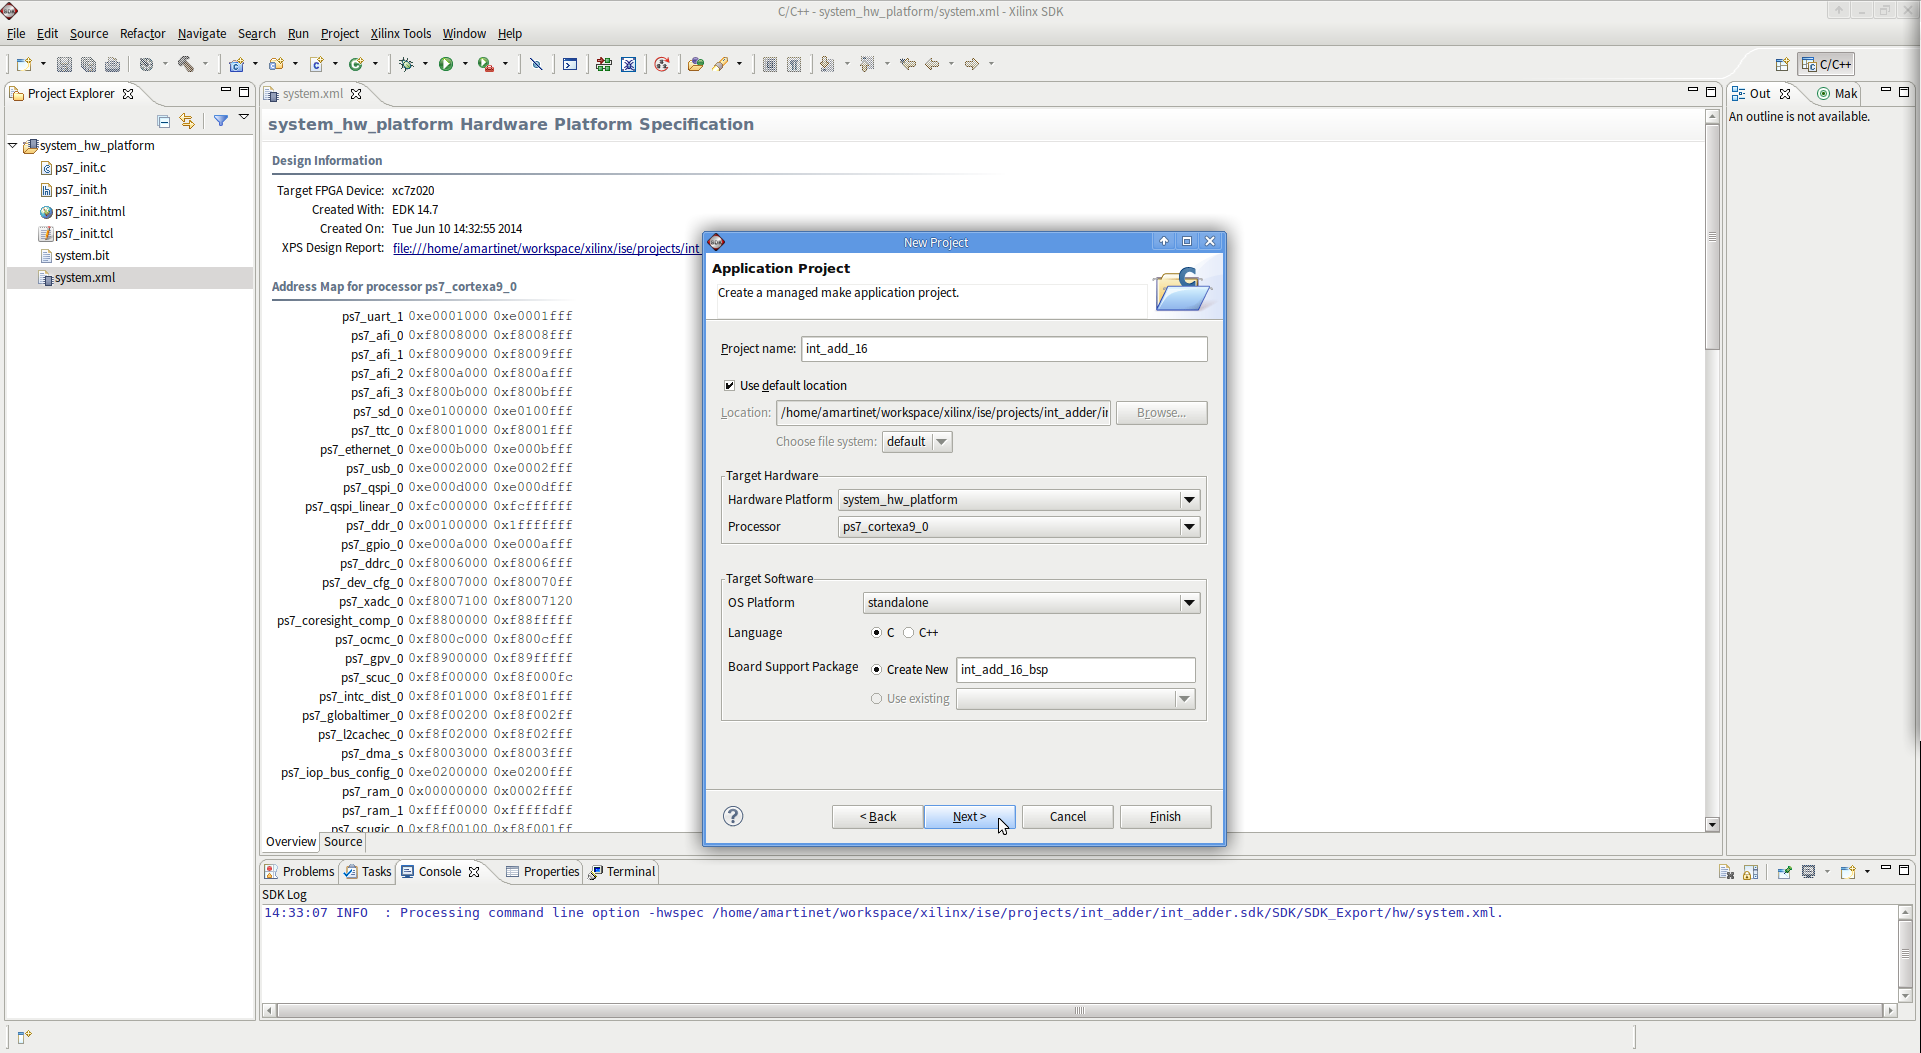
\includegraphics[scale=0.25]{pictures/XSDKNewProject2.png}
	\caption{Export hardware}
	\end{figure}
			\item Select the default "Hello World" template and click "Finish".
			Your project has been added in the project explorer.
			\item Expand it, expand the "src" folder and open "helloworld.c" double-clicking on
			it.
	\begin{figure}
	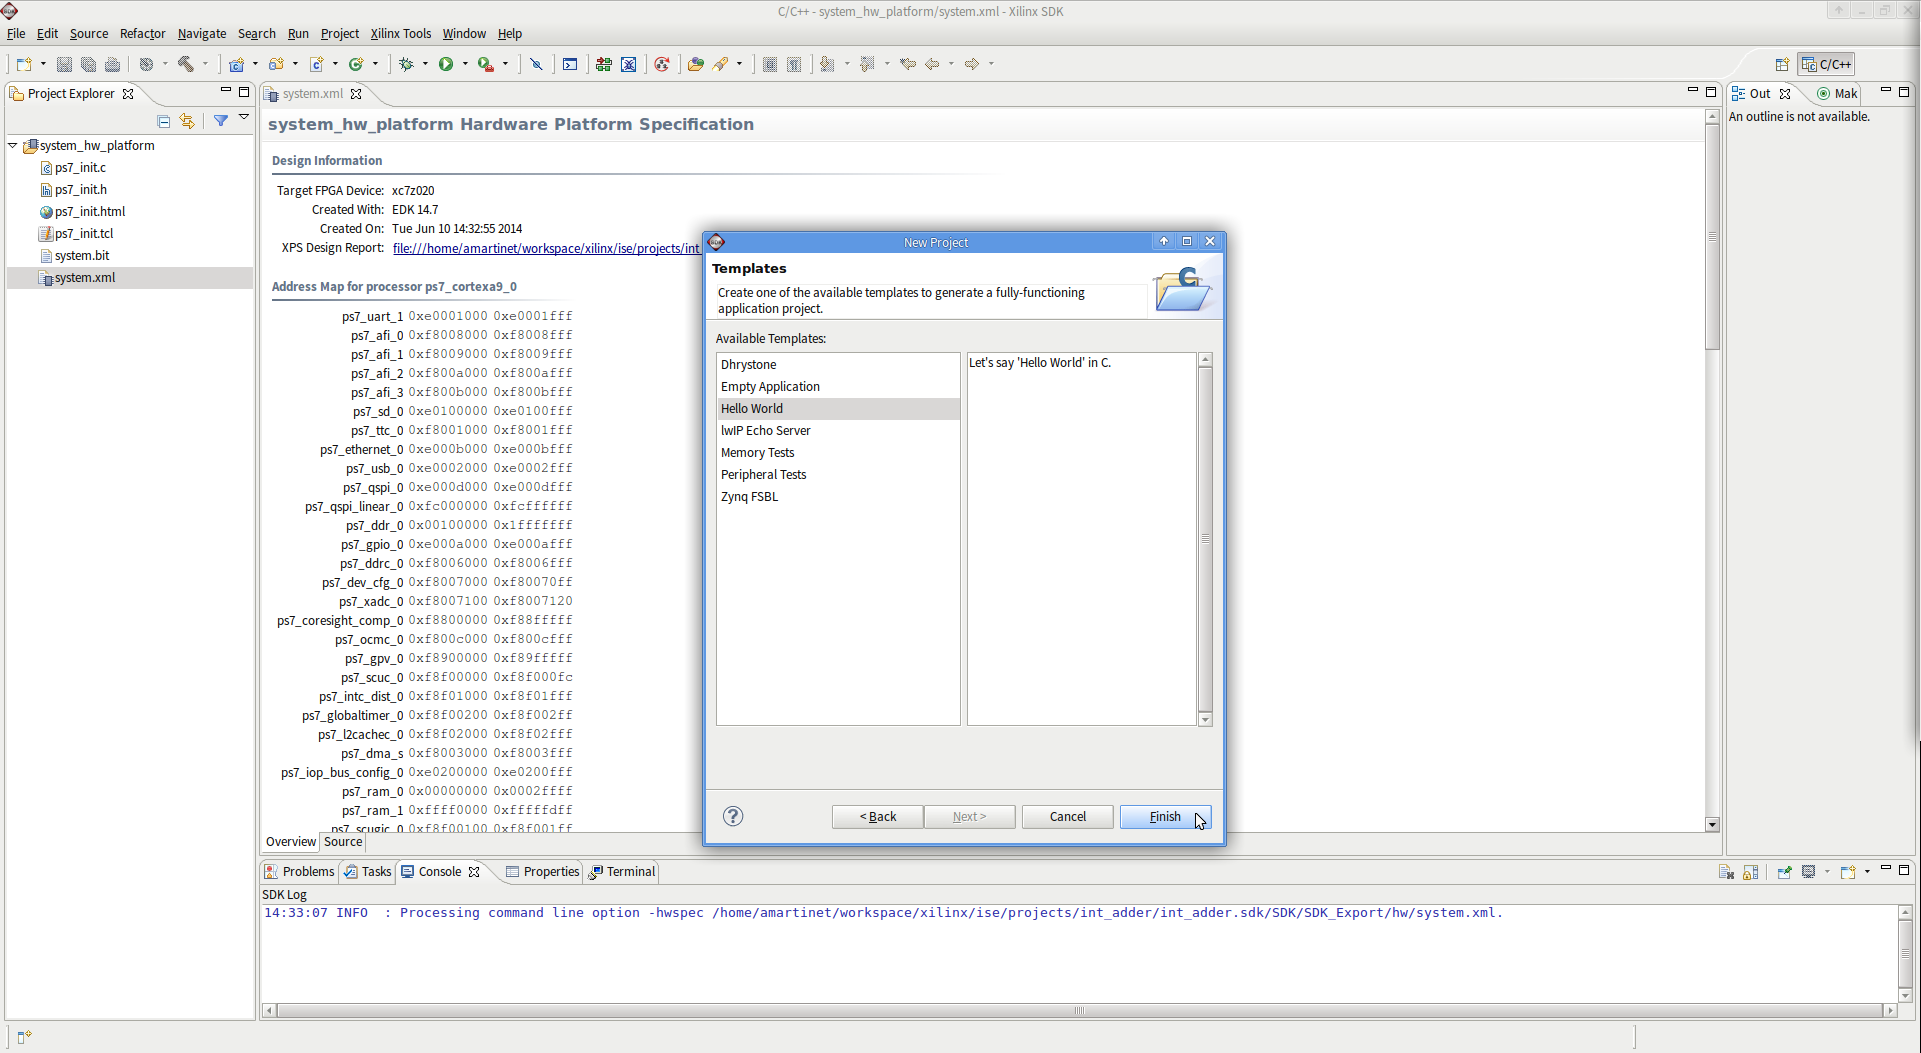
\includegraphics[scale=0.25]{pictures/XSDKNewProject3.png}
	\caption{Export hardware}
	\end{figure}
			\item You see that you can now display "Hello World". That's fine,
			but we have to get more deeper.
			\end{enumerate}
		\subsection{Peripheral communication}
		The only thing you need to know about peripheral communication is that
		GPIO commuication is done through registers. You can find full
		documentation here at
		\url{http://www.xilinx.com/support/documentation/user\_guides/ug585-Zynq-7000-TRM.pdf}.
		
		So what you need to use is writing/reading routines, that fortunately
		are provided by drivers in the
		int\_add\_16\_bsp/ps7\_cortexa9\_0/include directory. Here I will use
		the XGpioPs\_ReadReg() and XGpioPs\_WriteReg() macros from the xgpiops\_hw.h
		driver. These macros need a base address, which will be the base gpio
		address (0xE000A000, also defined as XPAR\_PS7\_GPIO\_0\_BASEADDR in
				xparameters.h), and an offset address, to compute the register to
		write/read on/from. Read macro returns the value read and Write macro
		needs of course the data (32 bit width) to write.

		Now we know how to read/write in a register, let's take a look on where
		to read/write. According to the documentation, ug585-Zynq-7000-TRM.pdf,
		the register to write is here DATA\_2 (we are on Bank 2, input register,
				so output from the chip point of view) (offset 0x48, absolute
					address 0xE000A048). You can also perform writing using the
				maskable output registers, but we don't use masks, as it is
				useless for this job. But first, need to enable output 
				(so FPGA output) writing 1 to the DIRM\_2 register. You will the
				write 0xFFFFFFFF to it, and will be able to write on the full
				DATA\_2 register.
				Reading is a much more simple. You just need to read using the
				routine and will get the full DATA\_2\_RO register value. (offset 0x68, absolute address
						0xE000A068).
		Now you can perform the full adder testing, and check the addition is
		well done. You will find the code I used to test in
		\hyperref[sec:CODE]{ appendix \ref{sec:CODE}: \nameref{sec:CODE} }.
	\subsection{Board programming and program running}
	Now you have a good and useful code, you need to program the board and run
	your application.
	\subsubsection{Program the board}
		To program the board and read from it, you need your 2 usb/micro-usb
		cables plugged on the PROG (J17) and UART (J14) usb ports.
		\begin{enumerate}
		\item Connect them and the AC power supply. Power the zedboard using the
		POWER (SW8) switch.
		\item Then you can connect a console through the JTAG usb cable (UART), using the
		shell command:
		\begin{alltt}
		\$ screen /dev/serial/by-id/usb-2012\_Cypress\_Semiconductor\_
		Cypress-USB2UART-Ver1.0G\_027211C91A19-if00 115200
		\end{alltt}
	\begin{figure}
	\begin{center}
	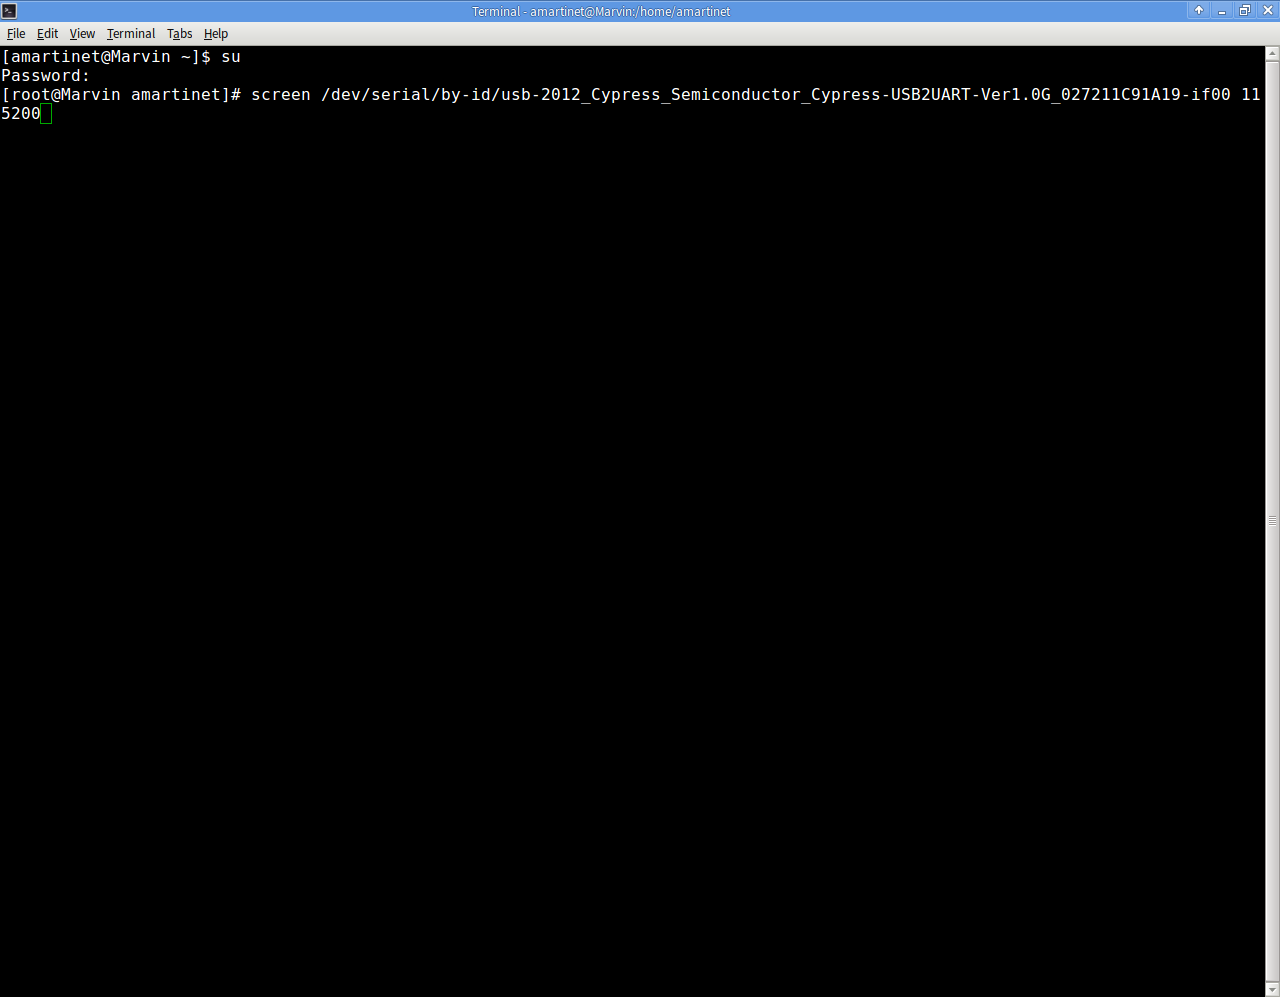
\includegraphics[scale=0.25]{pictures/ListenToPort.png}
	\end{center}
	\caption{Listening to ZedBoard's port}
	\end{figure}
		You obtain a black screen because no application is running.
		\item Back to SDK, you can put the bitstream into the FPGA. Click
		"Xilinx Tools" -> "Program FPGA". SDK wants to know what file to input.
		Keep the default one, which is the one that PlanAhead gived to SDK when
		you performed the "Export Hardware" action.
		\item Click "Program". Wait for the process to complete. The blue led
		wakes up on the board, telling you that you can now run your application
		with a functionnal FPGA.
	\begin{figure}
	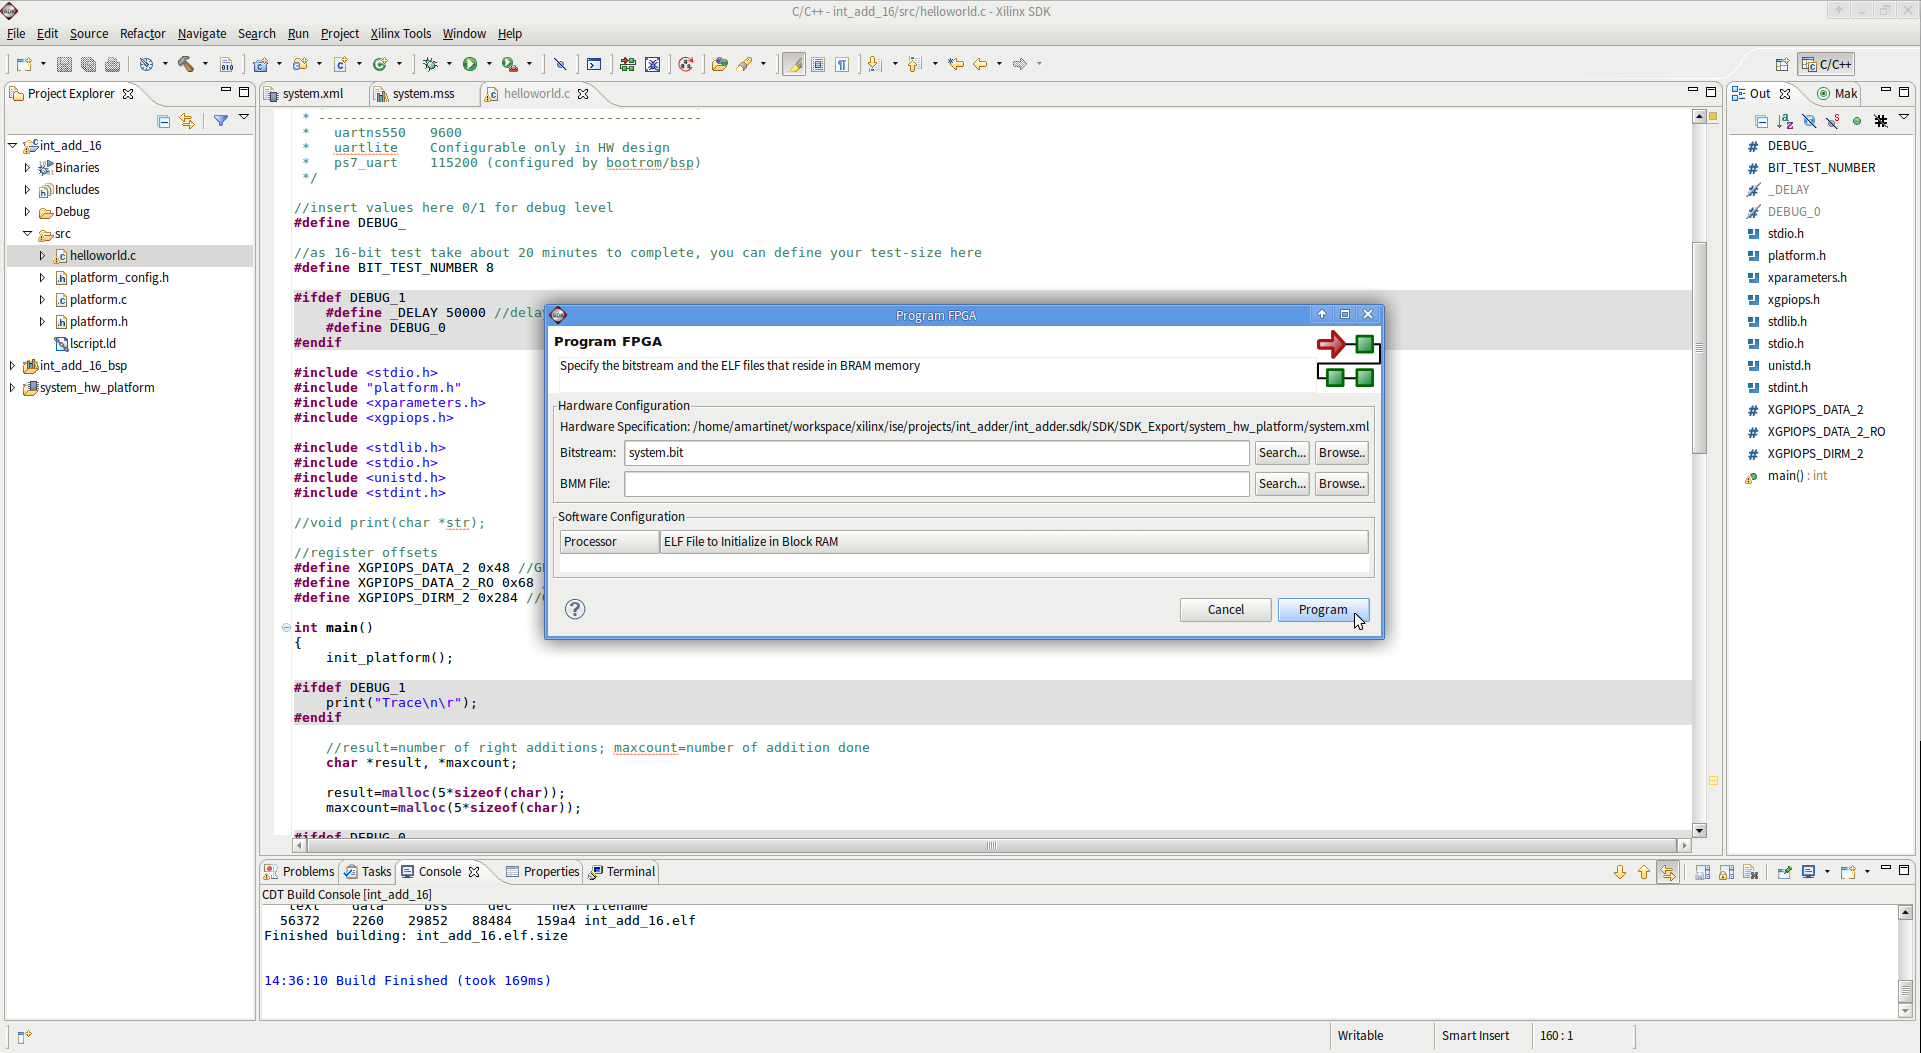
\includegraphics[scale=0.25]{pictures/ProgramFPGA1.png}
	\caption{Program FPGA}
	\end{figure}
		\item Before running your application, you must set a run configuration.
		There are several methods to do that. You can pass throught the run
		button, the "Run" menu, or right click on the project in the "Project
		Explorer" panel and choose the "Run As" option. Following one of these
		methods, click "Run Configurations". The wizard pops up.
		\item Right click on "Xilinx C/C++ application (GDB)", and click new.
		\item In the "Device Initialization" tab, check that the default "Reset
		Type" is set to "Reset Processor Only".
	\begin{figure}
	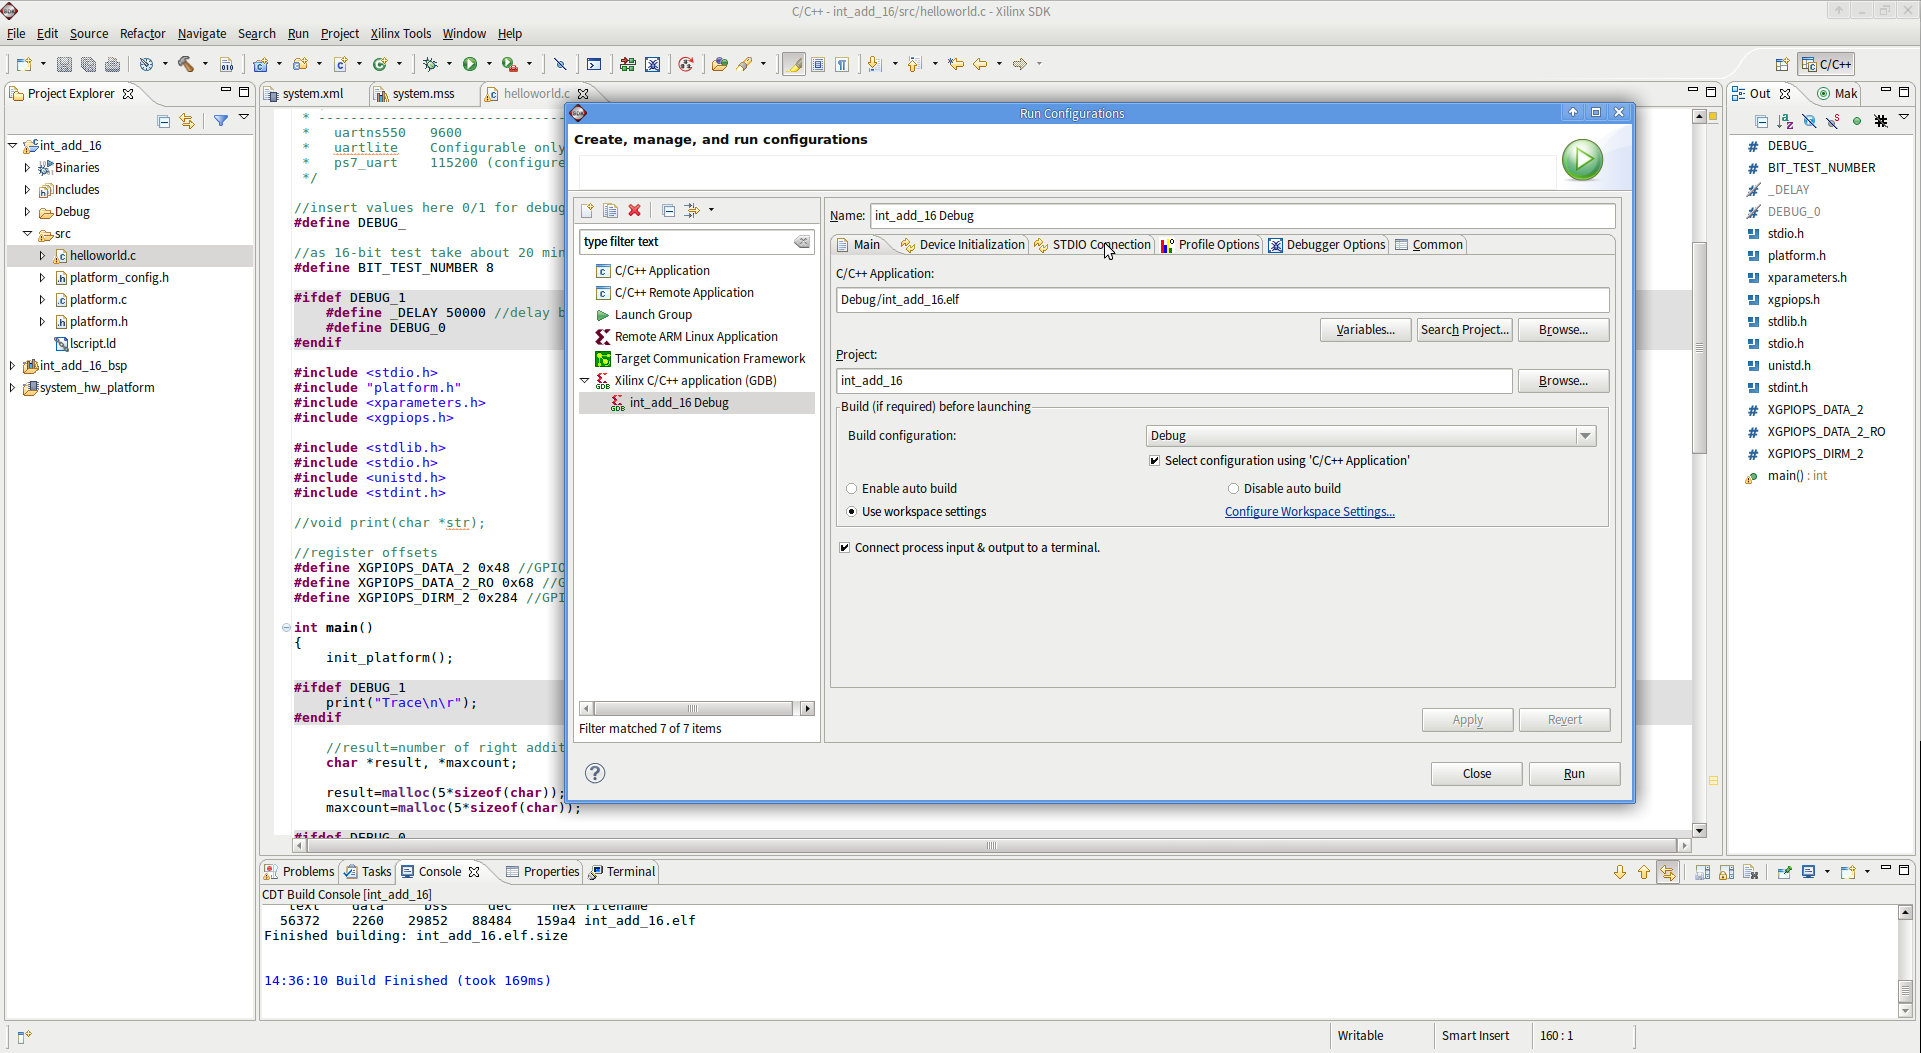
\includegraphics[scale=0.25]{pictures/RunConfig1.png}
	\caption{Run configuration}
	\end{figure}
		\item In the "STDIO Connection" tab, check the "Connect STDIO to Console"
		and leave the defaults: "Port: /dev/ttyS0", "BAUD Rate: 9600", so that
		the board connects to the tty you will be looking at, and so you will be
		able to see outputs.
	\begin{figure}[!h]
	\includegraphics[scale=0.25]{pictures/RunConfig2.png}
	\caption{Run configuration}
	\end{figure}
		\item Click "Apply".
		\item Then click "Run". Check the output. You will now see if you know
		how to add on 16 bits or not. (and actually, you do know!)
	\begin{figure}[!h]
	\includegraphics[scale=0.25]{pictures/Run.png}
	\caption{Run application}
	\end{figure}
	\begin{figure}[!h]
	\begin{center}
	\includegraphics[scale=0.25]{pictures/RunTrueResult.png}
	\end{center}
	\caption{Run result on 8 bits test}
	\end{figure}
		\end{enumerate}
		\newpage
\begin{appendices}
\section{Code listing: helloworld.c}
	\label{sec:CODE}
		\begin{alltt}
		\lstinputlisting{src/helloworld.c}
		\end{alltt}
\section{GPIO start guide}
\label{sec:GPIOSG}
	What you need to know about GPIO is pretty simple. There are 4 GPIO banks on
	the zedboard.
	The GPIO banks 0 and 1 are connected to MIO pins that are 54 bits large. So
	GPIO Bank 0 has a width of 32 bits and GPIO bank 1 22 bits. These are not
	useful as they are not connected to the Programable Logic (PL).
	GPIO Banks 2 and 3 are both 32 bits large and are connected to the EMIO
	interface to the PL. Note that they are plugged contiguesly (Bank 2 is 31:0
			pins of EMIO and Bank 3 is 63:32 pins of EMIO).
	The following schematic tells you how GPIO banks are organized. \\
	\begin{figure}[!h]
	\begin{center}
	\includegraphics{pictures/GPIOBD.png}
	\caption{GPIO Block Diagram}
	\end{center}
	\end{figure}
	
	Then, you will want to know how to access GPIO. This is pretty simple as you
	just access the registers decribed on the picture below.
	\begin{figure}[!h]
	\begin{center}
	\includegraphics[scale=0.7]{pictures/GPIOChannel.png}
	\end{center}
	\caption{GPIO Channel}
	\end{figure}
	As you can see, the DATA\_RO register is used to gather ingormation from
	GPIO devices. so we use it as input. You can see that the DATA,
	MASK\_DATA\_LSW, and MASK\_DATA\_MSW registers correspond to the same output
	register (chip point of view taken).
	Then you can see the DIRM and OEN register which can enable output and so
	writing operations on GPIO devices. As you can see, there is a bitwise and
	between this two registers. You might pay attention to that if you are using
	regular GPIO. You can also see various interrupts configuration registers
	that I don't use in this tutorial. \\


	Of course, you will get much better information using the original
	documentation. You will find it here, as I mentionned earlier:\\
		\url{http://www.xilinx.com/support/documentation/user\_guides/ug585-Zynq-7000-TRM.pdf}


\section{Known bugs}
	\subsection{JTAG connection}
	Though your USB-JTAG driver may be well installed and configured on your
	computer, the JTAG connection might be instable. This sometimes could be
	resolved by different ways:
	\begin{itemize}
		\item connect after programming FPGA
		\item connect just right after launching the application (with risk to
				miss some outputs)
		\item recompile all the hardware and re-import bitstream
		\item close all the project and re-open software
		\item reboot the pc
	\end{itemize}
	\subsection{Manjaro/Arch Linux issues}
	Issues have been found on Manjaro 3.10.40-1, when output to console fails
	when computer AC/DC power suppply converter is not plugged. This could be
	workaround by hard-resetting the zedboard using the power switch, then
	downloading the bitstream, strarting the application and then connecting
	your console to the board. Of course, you might loose some of the results,
	but for this test it should be fine.

\end{appendices}

	


\end{document}
